% Generated fragments require trusted human review before compilation.
% This binder never requests shell escape or runs external tools.
\documentclass[11pt]{article}
% Trusted shared apparatus. Requires LuaLaTeX; never use shell escape.
\usepackage{fontspec}
\defaultfontfeatures{Ligatures=TeX}
\IfFontExistsTF{Noto Serif}{\setmainfont{Noto Serif}}{%
  \IfFontExistsTF{DejaVu Serif}{\setmainfont{DejaVu Serif}}{%
    \IfFontExistsTF{Times New Roman}{\setmainfont{Times New Roman}}{%
      \PackageError{gelfand-binder}{No configured Cyrillic serif font installed}{Install Noto Serif or DejaVu Serif, or select an installed Cyrillic font.}%
    }%
  }%
}
\IfFontExistsTF{Noto Sans}{\setsansfont{Noto Sans}}{%
  \IfFontExistsTF{DejaVu Sans}{\setsansfont{DejaVu Sans}}{\setsansfont{Arial}}%
}
\IfFontExistsTF{Noto Sans Mono}{\setmonofont{Noto Sans Mono}}{%
  \IfFontExistsTF{DejaVu Sans Mono}{\setmonofont{DejaVu Sans Mono}}{\setmonofont{Courier New}}%
}
\usepackage[a4paper,margin=22mm]{geometry}
\usepackage{amsmath,amssymb,amsthm,mathtools}
\usepackage{xcolor}
\usepackage{tikz}
\usepackage{tikz-cd}
\usetikzlibrary{arrows.meta,positioning,calc}
\usepackage{hyperref}
\hypersetup{unicode=true,colorlinks=true,linkcolor=blue,pdftitle={Gelfand transcription binder}}
\newtheorem{theorem}{Theorem}
\newtheorem{lemma}{Lemma}
\newtheorem{proposition}{Proposition}
\newtheorem{corollary}{Corollary}
\theoremstyle{definition}
\newtheorem{definition}{Definition}
\newtheorem{example}{Example}
\theoremstyle{remark}
\newtheorem{remark}{Remark}
\setlength{\parindent}{0pt}
\setlength{\parskip}{0.55em}
\setlength{\emergencystretch}{3em}
\newcommand{\SourcePage}[2]{%
  \clearpage\phantomsection\label{#1:source-page}%
  \addcontentsline{toc}{subsection}{#1}%
  {\small\sffamily\color{blue!60!black}Source scan frame: #1; visible page/leaf label: #2}\par\medskip%
}
\newcommand{\Unclear}[3]{%
  \begingroup\color{orange!70!black}%
  [Unresolved reading #1/#2: #3]\endgroup%
}
\newcommand{\Incomplete}[3]{%
  \par\begingroup\color{red!65!black}\textbf{Incomplete #1/#2:} #3\endgroup\par%
}
\newcommand{\SourceFigure}[3]{%
  \par\begingroup\color{blue!60!black}\textbf{\hyperref[#1:source-page]{Source figure #1/#2}:} #3%
  \par\textit{Consult the authoritative scan at this locator.}\endgroup\par%
}



% Reader layout only. Original diplomatic text is retained verbatim.
\setlength{\parskip}{0.35em}
\setlength{\emergencystretch}{4em}
\renewcommand{\SourcePage}[2]{%
  \par\addvspace{1em}\phantomsection\label{#1:source-page}%
  \addcontentsline{toc}{subsection}{#1}%
  {\footnotesize\sffamily\color{blue!55!black}#1%
    \def\givenlabel{#2}\def\nolabel{unlabelled}%
    \ifx\givenlabel\nolabel\else\quad[номер в источнике: #2]\fi
  }\par\nobreak\smallskip%
}
\renewcommand{\Unclear}[3]{%
  \begingroup\color{orange!65!black}%
  \ifmmode\text{[неясно: #3]}\else[неясно: #3]\fi\endgroup%
}
\renewcommand{\Incomplete}[3]{%
  \par\begingroup\color{red!60!black}\textbf{Неразобранный фрагмент:} #3%
  \endgroup\par%
}
\renewcommand{\SourceFigure}[3]{%
  \par\begingroup\color{blue!55!black}\textbf{Рисунок:} #3%
  \par{\small\textit{Исходный рисунок: \hyperref[#1:source-page]{#1}, #2.}}%
  \endgroup\par%
}
\hypersetup{pdftitle={Семинар И. М. Гельфанда. Дипломатическая транскрипция},pdfauthor={},pdfsubject={Русское рабочее издание с отмеченными сомнительными чтениями}}

\usepackage[normalem]{ulem}
\usepackage{newunicodechar}
\usepackage{adjustbox}
\newfontfamily\SourceSymbolFont{Segoe UI Symbol}
\newfontfamily\SourceCJKFont{MS Gothic}
\let\DiplomaticMathUnderline\underline
\renewcommand{\underline}[1]{\ifmmode\DiplomaticMathUnderline{#1}\else\uline{#1}\fi}
\newunicodechar{→}{\ifmmode\text{{\SourceSymbolFont\char"2192}}\else{\SourceSymbolFont\char"2192}\fi}
\newunicodechar{⇒}{\ifmmode\text{{\SourceSymbolFont\char"21D2}}\else{\SourceSymbolFont\char"21D2}\fi}
\newunicodechar{∀}{\ifmmode\text{{\SourceSymbolFont\char"2200}}\else{\SourceSymbolFont\char"2200}\fi}
\newunicodechar{∂}{\ifmmode\text{{\SourceSymbolFont\char"2202}}\else{\SourceSymbolFont\char"2202}\fi}
\newunicodechar{∈}{\ifmmode\text{{\SourceSymbolFont\char"2208}}\else{\SourceSymbolFont\char"2208}\fi}
\newunicodechar{∌}{\ifmmode\text{{\SourceSymbolFont\char"220C}}\else{\SourceSymbolFont\char"220C}\fi}
\newunicodechar{√}{\ifmmode\text{{\SourceSymbolFont\char"221A}}\else{\SourceSymbolFont\char"221A}\fi}
\newunicodechar{∞}{\ifmmode\text{{\SourceSymbolFont\char"221E}}\else{\SourceSymbolFont\char"221E}\fi}
\newunicodechar{∧}{\ifmmode\text{{\SourceSymbolFont\char"2227}}\else{\SourceSymbolFont\char"2227}\fi}
\newunicodechar{∩}{\ifmmode\text{{\SourceSymbolFont\char"2229}}\else{\SourceSymbolFont\char"2229}\fi}
\newunicodechar{∪}{\ifmmode\text{{\SourceSymbolFont\char"222A}}\else{\SourceSymbolFont\char"222A}\fi}
\newunicodechar{∫}{\ifmmode\text{{\SourceSymbolFont\char"222B}}\else{\SourceSymbolFont\char"222B}\fi}
\newunicodechar{∴}{\ifmmode\text{{\SourceSymbolFont\char"2234}}\else{\SourceSymbolFont\char"2234}\fi}
\newunicodechar{∼}{\ifmmode\text{{\SourceSymbolFont\char"223C}}\else{\SourceSymbolFont\char"223C}\fi}
\newunicodechar{≈}{\ifmmode\text{{\SourceSymbolFont\char"2248}}\else{\SourceSymbolFont\char"2248}\fi}
\newunicodechar{≠}{\ifmmode\text{{\SourceSymbolFont\char"2260}}\else{\SourceSymbolFont\char"2260}\fi}
\newunicodechar{≤}{\ifmmode\text{{\SourceSymbolFont\char"2264}}\else{\SourceSymbolFont\char"2264}\fi}
\newunicodechar{≥}{\ifmmode\text{{\SourceSymbolFont\char"2265}}\else{\SourceSymbolFont\char"2265}\fi}
\newunicodechar{⊕}{\ifmmode\text{{\SourceSymbolFont\char"2295}}\else{\SourceSymbolFont\char"2295}\fi}
\newunicodechar{⊗}{\ifmmode\text{{\SourceSymbolFont\char"2297}}\else{\SourceSymbolFont\char"2297}\fi}
\newunicodechar{①}{\ifmmode\text{{\SourceSymbolFont\char"2460}}\else{\SourceSymbolFont\char"2460}\fi}
\newunicodechar{②}{\ifmmode\text{{\SourceSymbolFont\char"2461}}\else{\SourceSymbolFont\char"2461}\fi}
\newunicodechar{③}{\ifmmode\text{{\SourceSymbolFont\char"2462}}\else{\SourceSymbolFont\char"2462}\fi}
\newunicodechar{④}{\ifmmode\text{{\SourceSymbolFont\char"2463}}\else{\SourceSymbolFont\char"2463}\fi}
\newunicodechar{Ⓗ}{\ifmmode\text{{\SourceSymbolFont\char"24BD}}\else{\SourceSymbolFont\char"24BD}\fi}
\newunicodechar{〃}{\ifmmode\text{{\SourceCJKFont\char"3003}}\else{\SourceCJKFont\char"3003}\fi}


% Reader revision 3. Annotation wording and candidates remain unchanged.
\usetikzlibrary{shapes.geometric,decorations.pathreplacing,decorations.markings,patterns,fit}
\newsavebox{\ReaderAnnotationBox}
\newcommand{\ReaderAnnotation}[1]{%
  \sbox{\ReaderAnnotationBox}{[неясно: #1]}%
  \ifdim\wd\ReaderAnnotationBox>.70\linewidth
    \parbox[t]{.70\linewidth}{\raggedright[неясно: #1]}%
  \else\usebox{\ReaderAnnotationBox}\fi%
}
\ExplSyntaxOn
\cs_new_protected:Npn \reader_unclear_candidate:n #1
 {
  \tl_set:Nx \l_tmpa_tl { \tl_to_str:n {#1} }
  % Text explicitly guarded inside a mathematical candidate remains math-safe.
  \regex_replace_all:nnN { \\(?:text|textrm|textnormal|textbf|operatorname)\s*\{[^{}]*\} } { } \l_tmpa_tl
  \regex_match:nVTF { [\x{0400}-\x{052F}] | \$ } \l_tmpa_tl
   { \ifmmode \text{\ReaderAnnotation{#1}} \else \ReaderAnnotation{#1} \fi }
   {
    \ifmmode
      [\text{неясно:~}#1]
    \else
      \regex_match:nVTF { [_^] | \\ } \l_tmpa_tl
       { \ensuremath{[\text{неясно:~}#1]} }
       { \ReaderAnnotation{#1} }
    \fi
   }
 }
\RenewDocumentCommand \Unclear { m m m }
 { \begingroup\color{orange!65!black}\reader_unclear_candidate:n{#3}\endgroup }
\ExplSyntaxOff
\newsavebox{\ReaderIncompleteBox}
\newcommand{\ReaderIncompleteNote}[1]{%
 \sbox{\ReaderIncompleteBox}{\textbf{Неразобранный фрагмент:} #1}%
 \ifdim\wd\ReaderIncompleteBox>.70\linewidth
  \parbox[t]{.70\linewidth}{\raggedright\textbf{Неразобранный фрагмент:} #1}%
 \else\usebox{\ReaderIncompleteBox}\fi%
}
\renewcommand{\Incomplete}[3]{%
 \ifmmode\text{\color{red!60!black}\ReaderIncompleteNote{#3}}%
 \else\par\begingroup\color{red!60!black}\textbf{Неразобранный фрагмент:} #3\endgroup\par\fi%
}
% Ragged right avoids stretching long untranslated abbreviations into margins.
\AtBeginDocument{\raggedright}
\newunicodechar{А}{\ifmmode\text{\char"410\relax}\else\char"410\relax\fi}
\newunicodechar{Б}{\ifmmode\text{\char"411\relax}\else\char"411\relax\fi}
\newunicodechar{В}{\ifmmode\text{\char"412\relax}\else\char"412\relax\fi}
\newunicodechar{Г}{\ifmmode\text{\char"413\relax}\else\char"413\relax\fi}
\newunicodechar{Д}{\ifmmode\text{\char"414\relax}\else\char"414\relax\fi}
\newunicodechar{Е}{\ifmmode\text{\char"415\relax}\else\char"415\relax\fi}
\newunicodechar{Ж}{\ifmmode\text{\char"416\relax}\else\char"416\relax\fi}
\newunicodechar{З}{\ifmmode\text{\char"417\relax}\else\char"417\relax\fi}
\newunicodechar{И}{\ifmmode\text{\char"418\relax}\else\char"418\relax\fi}
\newunicodechar{Й}{\ifmmode\text{\char"419\relax}\else\char"419\relax\fi}
\newunicodechar{К}{\ifmmode\text{\char"41A\relax}\else\char"41A\relax\fi}
\newunicodechar{Л}{\ifmmode\text{\char"41B\relax}\else\char"41B\relax\fi}
\newunicodechar{М}{\ifmmode\text{\char"41C\relax}\else\char"41C\relax\fi}
\newunicodechar{Н}{\ifmmode\text{\char"41D\relax}\else\char"41D\relax\fi}
\newunicodechar{О}{\ifmmode\text{\char"41E\relax}\else\char"41E\relax\fi}
\newunicodechar{П}{\ifmmode\text{\char"41F\relax}\else\char"41F\relax\fi}
\newunicodechar{Р}{\ifmmode\text{\char"420\relax}\else\char"420\relax\fi}
\newunicodechar{С}{\ifmmode\text{\char"421\relax}\else\char"421\relax\fi}
\newunicodechar{Т}{\ifmmode\text{\char"422\relax}\else\char"422\relax\fi}
\newunicodechar{У}{\ifmmode\text{\char"423\relax}\else\char"423\relax\fi}
\newunicodechar{Ф}{\ifmmode\text{\char"424\relax}\else\char"424\relax\fi}
\newunicodechar{Х}{\ifmmode\text{\char"425\relax}\else\char"425\relax\fi}
\newunicodechar{Ц}{\ifmmode\text{\char"426\relax}\else\char"426\relax\fi}
\newunicodechar{Ч}{\ifmmode\text{\char"427\relax}\else\char"427\relax\fi}
\newunicodechar{Ш}{\ifmmode\text{\char"428\relax}\else\char"428\relax\fi}
\newunicodechar{Щ}{\ifmmode\text{\char"429\relax}\else\char"429\relax\fi}
\newunicodechar{Ъ}{\ifmmode\text{\char"42A\relax}\else\char"42A\relax\fi}
\newunicodechar{Ы}{\ifmmode\text{\char"42B\relax}\else\char"42B\relax\fi}
\newunicodechar{Ь}{\ifmmode\text{\char"42C\relax}\else\char"42C\relax\fi}
\newunicodechar{Э}{\ifmmode\text{\char"42D\relax}\else\char"42D\relax\fi}
\newunicodechar{Ю}{\ifmmode\text{\char"42E\relax}\else\char"42E\relax\fi}
\newunicodechar{Я}{\ifmmode\text{\char"42F\relax}\else\char"42F\relax\fi}
\newunicodechar{а}{\ifmmode\text{\char"430\relax}\else\char"430\relax\fi}
\newunicodechar{б}{\ifmmode\text{\char"431\relax}\else\char"431\relax\fi}
\newunicodechar{в}{\ifmmode\text{\char"432\relax}\else\char"432\relax\fi}
\newunicodechar{г}{\ifmmode\text{\char"433\relax}\else\char"433\relax\fi}
\newunicodechar{д}{\ifmmode\text{\char"434\relax}\else\char"434\relax\fi}
\newunicodechar{е}{\ifmmode\text{\char"435\relax}\else\char"435\relax\fi}
\newunicodechar{ж}{\ifmmode\text{\char"436\relax}\else\char"436\relax\fi}
\newunicodechar{з}{\ifmmode\text{\char"437\relax}\else\char"437\relax\fi}
\newunicodechar{и}{\ifmmode\text{\char"438\relax}\else\char"438\relax\fi}
\newunicodechar{й}{\ifmmode\text{\char"439\relax}\else\char"439\relax\fi}
\newunicodechar{к}{\ifmmode\text{\char"43A\relax}\else\char"43A\relax\fi}
\newunicodechar{л}{\ifmmode\text{\char"43B\relax}\else\char"43B\relax\fi}
\newunicodechar{м}{\ifmmode\text{\char"43C\relax}\else\char"43C\relax\fi}
\newunicodechar{н}{\ifmmode\text{\char"43D\relax}\else\char"43D\relax\fi}
\newunicodechar{о}{\ifmmode\text{\char"43E\relax}\else\char"43E\relax\fi}
\newunicodechar{п}{\ifmmode\text{\char"43F\relax}\else\char"43F\relax\fi}
\newunicodechar{р}{\ifmmode\text{\char"440\relax}\else\char"440\relax\fi}
\newunicodechar{с}{\ifmmode\text{\char"441\relax}\else\char"441\relax\fi}
\newunicodechar{т}{\ifmmode\text{\char"442\relax}\else\char"442\relax\fi}
\newunicodechar{у}{\ifmmode\text{\char"443\relax}\else\char"443\relax\fi}
\newunicodechar{ф}{\ifmmode\text{\char"444\relax}\else\char"444\relax\fi}
\newunicodechar{х}{\ifmmode\text{\char"445\relax}\else\char"445\relax\fi}
\newunicodechar{ц}{\ifmmode\text{\char"446\relax}\else\char"446\relax\fi}
\newunicodechar{ч}{\ifmmode\text{\char"447\relax}\else\char"447\relax\fi}
\newunicodechar{ш}{\ifmmode\text{\char"448\relax}\else\char"448\relax\fi}
\newunicodechar{щ}{\ifmmode\text{\char"449\relax}\else\char"449\relax\fi}
\newunicodechar{ъ}{\ifmmode\text{\char"44A\relax}\else\char"44A\relax\fi}
\newunicodechar{ы}{\ifmmode\text{\char"44B\relax}\else\char"44B\relax\fi}
\newunicodechar{ь}{\ifmmode\text{\char"44C\relax}\else\char"44C\relax\fi}
\newunicodechar{э}{\ifmmode\text{\char"44D\relax}\else\char"44D\relax\fi}
\newunicodechar{ю}{\ifmmode\text{\char"44E\relax}\else\char"44E\relax\fi}
\newunicodechar{я}{\ifmmode\text{\char"44F\relax}\else\char"44F\relax\fi}
\newunicodechar{Ё}{\ifmmode\text{\char"401\relax}\else\char"401\relax\fi}
\newunicodechar{ё}{\ifmmode\text{\char"451\relax}\else\char"451\relax\fi}


% Reader-only pairing support; accepted raw bodies remain unchanged.
\RequirePackage{graphicx}
\RequirePackage{adjustbox}
\newcommand{\ReaderOriginalPanel}[2]{%
  \begin{minipage}[t]{.48\linewidth}\vspace{0pt}\centering
    \includegraphics[width=\linewidth,keepaspectratio]{#1}\par\smallskip
    {\scriptsize Оригинал рукописного рисунка: #2}\par
  \end{minipage}%
}
\newcommand{\ReaderDiagramPair}[3]{%
  \par\noindent\begingroup
  \ReaderOriginalPanel{#1}{#2}\hfill
  \begin{minipage}[t]{.48\linewidth}\vspace{0pt}\centering
    {\scriptsize Типографское воссоздание}\par\smallskip
    \begin{adjustbox}{max width=\linewidth}#3\end{adjustbox}\par
  \end{minipage}%
  \endgroup\par\smallskip
}
\newcommand{\ReaderDescriptionPair}[3]{%
  \par\noindent\begingroup
  \ReaderOriginalPanel{#1}{#2}\hfill
  \begin{minipage}[t]{.48\linewidth}\vspace{0pt}\raggedright
    {\scriptsize Типографское описание}\par\smallskip
    #3\par
  \end{minipage}%
  \endgroup\par\smallskip
}


\begin{document}
\begin{center}
{\Large Семинар И. М. Гельфанда}\par\medskip
{\LARGE Дипломатическая транскрипция}\par\bigskip
{\large Рабочее русское издание}\par\medskip
{\large Том 02 из 34. Архивная глава 002}\par\bigskip
Кадры GELFAND-P000140 -- GELFAND-P000207\par
\end{center}
\medskip
Сокращения, отменённые записи и сомнительные чтения сохранены.
Неразобранные фрагменты отмечены в тексте. Математические утверждения
источника переданы без молчаливых исправлений.

В текущем комплекте приняты 165 из 165 возвратов; учтены 1527 из 1527 кадров. Кадров без принятого возврата: 0.
Статусы кадров в отчётах о полноте: транскрибированы 1168, неразборчивы 357, частично прочитаны 1, недоступны 1.
Нерешённых записей журнала чтений: 6820.
Статус «неразборчивый» может отмечать локальную утрату зачёркнутой записи;
он не означает отсутствия всего кадра.
Сверка с рукописью продолжается. Рабочие журналы чтений и происхождения
данных сохранены отдельно.

Ограничения исходного комплекта: повреждённый исходный скан GELFAND-P000722; каталожные записи 603, 694 без сканов; в архивной главе 029 не перечислена часть 25.

Границы кадров показаны небольшими синими указателями; печатный текст
продолжается без обязательного разрыва страницы после каждого кадра.
\bigskip\hrule\bigskip
\SourcePage{GELFAND-P000140}{5}
\underline{Семинар Гельфанда.} \underline{5/IX}

1. Систематически будет \underline{статфизика.} (Минлос)

2. Состояние \underline{псевдодифференциальных} операторов.
(Вишик и Агранович)

3. \underline{Алгебраические группы} (Кириллов)

\underline{Ценная информация:} лекции Atiyah по $K$-функтору
не требуют предв. знаний, кроме опред. топологич. пр-ва
и $n$-мерного векторного пр-ва
(По степени про-зрачности не сравнимо даже с Милнором)

4. \underline{Деформации} всякого рода. (условное название:
нелинейный анализ), в том числе \underline{Kodaira} и \underline{Spencer}.

\underline{Результат Hirzebruch'a.} (Гельфанд)
\begin{gather*}
\left\{\begin{aligned}
z_1^3+z_2^{3k-1}+z_3^2+z_4^2+z_5^2&=0\\
|z_1|^2+|z_2|^2+|z_3|^2+|z_4|^2+|z_5|^2&=\varepsilon
\end{aligned}\right.
\end{gather*}
[Справа обведено овалом $3k-1$.]
\Unclear{GELFAND-P000140}{z2-overwritten-exponent}{Показатель при $z_2$ начинается $3k$; конец густо переписан: $3k-1$ / иной переписанный конец.}
\Unclear{GELFAND-P000140}{modulus-overwrite}{Во второй строке правая черта и показатель при $|z_3|$ густо переписаны; $|z_3|^2$ дано с этой оговоркой. Между $|z_4|^2$ и $|z_5|^2$ знак похож на $+$, но густой.}

10 неизв. и [зачёркнуто перед $3$]
\Unclear{GELFAND-P000140}{cancelled-equation-count}{Зачёркнутый короткий фрагмент после «и»: $7$-подобный знак и дальнейшие густые штрихи; исходное содержание неразборчиво.}
3 ур-я

\underline{Милнор:} это гомеоморфно $S^7$

\underline{Хирцебрух:} при $k=1,2,\ldots,28$ там разные
дифф. структуры,
а дальше всё повторяется периодически и
это все милноровские сферы.

$S^{11}$ есть 992 штуки и они получаются
такими уравнениями.

\SourcePage{GELFAND-P000141}{unlabelled}
\underline{Bass} (Каждан) \underline{жёсткость арифм. подгрупп.}
\Unclear{GELFAND-P000141}{speaker-name}{Третья буква фамилии между «Ка» и «дан» написана густым соединённым штрихом: «Каждан» / «Каздан».}

$SL(n,Z)\subset SL(n,R)$ — жёсткая подгруппа,

[Зачёркнуты короткое начало строки и слово перед «всякая».]
\Unclear{GELFAND-P000141}{cancelled-introduction}{Начальное зачёркнутое обозначение похоже на «II.» / «Те.», следующее густо зачёркнутое слово не читается.}
всякая деформация, (т.е. отобр.) \fbox{$(n>2)$}
\begin{gather*}
SL(n,Z)\times[0,1]\longrightarrow SL(n,R)
\end{gather*}
к-рое непрерывно и $\forall t\in[0,1]$ гомоморфизм,
при $t=0$ это вложение) тривиальна, т.е. она
есть внутр. автоморфизм отн. $g(t)$ (кривая в группе)
\begin{gather*}
\varphi(h\times t)=g(t)h g(t)^{-1},\qquad h\in SL(n,Z)
\end{gather*}
Теорема Вейля док. лишь для случая, когда
факторпр-во компактно.

Зад. свод. к задаче о конгруэнцподгр. над конечным
полем.
(Если есть два гомоморф., то неизв., можно ли их
соединить)

Существ. деформ. — нетрив. $H^1(\Gamma,\mathfrak g)$
\Unclear{GELFAND-P000141}{cohomology-terminal}{После $H^1(\Gamma,\mathfrak g)$ стоят небольшие двоеточие- и звёздочка-подобные штрихи; их буквальное чтение не установлено.}
(Borel, Bass)
[Под $H^1$ стрелка вверх от «конечн. число образ.»]

$\mathfrak g$ — алгебра Ли.

В $\mathfrak g$ есть решётка целочисл. матриц $L$.
($L$ — решётка в алгебре Ли)
\begin{gather*}
H^1(\Gamma,\mathfrak g)=H^1(\Gamma,L)\underset Z\otimes R
\end{gather*}
Док., что $H^1(\Gamma,L)$ конечна,
Дост. док., что $\exists p$, такое что умн. на $p$ есть
эпиморфизм [под $p$ вписано и подчёркнуто «простое»]
\begin{gather*}
H^1(\Gamma,L)\overset p\longrightarrow H^1(\Gamma,L)
\longrightarrow H^1(\Gamma,L/pL)\\
(\text{из }0\longrightarrow L\overset p\longrightarrow L\longrightarrow L/pL\longrightarrow0)
\end{gather*}
Дост. док., что справа $0$.

Можно свести дело к случаю, когда $\Gamma$ конечна:
вместо $\Gamma$ — $\Gamma/[\Gamma_p,\Gamma_p]$,
$\Gamma_p$ — гр. элем., сравнимые с $1$
по модулю $p$.

\SourcePage{GELFAND-P000142}{6}
Итак, достат. доказать, что
\begin{gather*}
H^1(\Gamma/\Gamma_p,L/pL)=0
\end{gather*}
и всё свод. к кон. группам.
То же \underline{Borel} невероятно трудное док-во.
\underline{Bass} — лишь для расщепимых.

\underline{Смейл} (Аносов)

\underline{Арнольд.} \underline{$U$-система} (по Аносову)
$g:H\longrightarrow H$, если [под стрелкой «дифф.»]
\Unclear{GELFAND-P000142}{manifold-letter}{Буквы области и образа написаны $H$-подобно; $H$ / $M$. В точном определении ниже стоит $TM_x$.}
есть 2 напр. [два крестовидных рисунка: в каждом пересекаются
горизонтальная и вертикальная линии], по 1-му растяг., по другому
сжимает ($\leq$, $\geq$ оценки на сжатие и растяжение)
\Unclear{GELFAND-P000142}{stretch-contraction}{Последняя буква сокращения после «по 1-му» имеет густые соединённые штрихи: «растяг.» / «растяж.». Сокращение не развёрнуто.}

[Слева двойная вертикальная черта.]
\underline{Пример:} автом. тора, больше было неизвестно.
Смейл утвержд., что нашёл мн-зия, кроме тора и их
$U$-автом. и все такие автом. (гипотеза).

\underline{Точное опр.:} $\exists TM_x=X_x\oplus Y_x$, $\forall\xi\in X_x$,
$g^*\xi\in X_{gx}$,
[Под «Точное опр.»: «сущ. рим. метрика»]
\begin{gather*}
|g^*\xi|<\theta|\xi|,\quad0<\theta<1,\\
\forall\eta\in Y_x,\quad |g^*\eta|>\frac1\theta|\eta|.
\end{gather*}
(это $V$-каскад)
\Unclear{GELFAND-P000142}{u-v-designation}{Начальный заголовок имеет $U$, а здесь знак похож на $V$: $V$-каскад / $U$-каскад.}

\underline{Автом. тора} — соб. направления соотв. матрицы.

Все [зачёркнуто слово; снизу вставлено с охватывающей дугой
«новые примеры»] — фактор. ниль. группы по дискр. подгруппе.
\Unclear{GELFAND-P000142}{cancelled-examples-word}{Зачёркнутое слово после «Все» имеет с/ю/д-подобные остатки; исходное слово неразборчиво. Вставка «новые примеры» видима.}
(ниль-Мн-зия)

$G/\Gamma$, $G=$
\SourceFigure{GELFAND-P000142}{nilpotent-matrix}{Матрица в круглых скобках, шесть позиций на диагонали, два верхнетреугольных блока. Сверху $a,b$, ниже $c$; в нижнем блоке $a^*,b^*,c^*$; вне блоков два $0$. Диагональные густые знаки похожи на $1$ / точки. Геометрия блоков видима, буквальное чтение всех диагональных знаков не установлено.}
— 6-го порядка
\begin{gather*}
\Gamma=\left\{\begin{aligned}
a&=m+n\sqrt3,\qquad a^*=m-n\sqrt3,\\
b&=m'+n'\sqrt3,\qquad\text{[ряд повторительных штрихов]},\\
c&=m''+n''\sqrt3,
\end{aligned}\right.
\end{gather*}
[Справа охватывающая фигурная скобка.]
$G/\Gamma$ компактно.
\underline{Размерн. $3+3$}
сжим. и расшир.

\SourcePage{GELFAND-P000143}{unlabelled}
\underline{Собственно Аносов.}

Каскад — итерации дифф. гомеоморфизма
(с непр. временем — поток)
Описать типичные динамич. системы — каскады.
(всюду плотное мн-во, открытое)

\underline{Грубый поток} — перех. в экв. при малом $(C^1)$ возмущ.
(экв. — отлич. диффеом.)

\underline{2-мерн. случай:} \underline{теор. Андронова-Понтрягина} — описаны
грубые системы (конечн. число «устойч.» циклов и особ.
точек и сепаратрисы сёдел в общем положении —
— не пересек., не сов.) Их мн-во откр., плотное.

\underline{Система Андронова-Понтрягина.}

1. Кон. число полож. равн. и периодич. траекторий,
причём все они локально грубые (усл. на соб. знач. и
мультипликаторы)
(многомерный случай это уже нетрив.)

2. Сепаратрисы общего положения
(Усл.,
Условно устойч. мн-зия,
Асимпт. пучки,
орисферы,
орициклы)
(Мн-зия вход. и выходящих —
— см. Коддингтон и Левинсон)

3. Все траектории при $t\longrightarrow\pm\infty$ стремятся
к полож. равновесия и периодич. решениям.

[Две строки густо зачёркнуты прямыми и волнистыми линиями.]
\Unclear{GELFAND-P000143}{cancelled-fourth-condition}{Начальный перечёркнутый знак $4)$- / $\forall$-подобный; далее сохранились «сепаратр. общего полож.», «(не пересек.», $2$-подобный знак и «собр.»; снизу «это не очень» и густой конец. Полное первоначальное высказывание неразборчиво.}

\underline{4 утверждения.}
1. Все А.-П. — грубые — [справа обведён вопросительный знак]
2. Все грубые — А.-П.
3. А.-П. плотны
[Под пунктом 3 зачёркнуто «дру»-подобное начало в скобках.]
\Unclear{GELFAND-P000143}{cancelled-parenthesis}{Короткая зачёркнутая скобка под пунктом 3: «дру» / «друг» / неразборчиво.}
4. Грубые плотны
[Справа от пунктов 2–4 двойная вертикальная черта.]
Опровергнуты Смейлом.

\SourcePage{GELFAND-P000144}{7}
\underline{Грубая система:} $\dot w=f(w)$.
\begin{gather*}
\forall\varepsilon\ \exists\delta,\ \forall g,\ \|g-f\|_{C^1}<\delta,
\end{gather*}
$\exists\varepsilon$-гомеом., перев. траект. $f$
в траект. $g$.

Для каскада: коммут диагр
($\exists\varepsilon$-гомеом. $\chi$)
\SourceFigure{GELFAND-P000144}{conjugacy-square}{Четыре $M$ в квадрате. Верхняя стрелка вправо с $f$, нижняя вправо с $g$, обе боковые стрелки вниз; слева $\chi$, справа $\chi$ / $x$-подобный более короткий знак.}

(Для потоков естеств. считать, что может меняться скорость,
если это запретить, то грубых почти не остаётся)

\underline{Подмн-во $b|$ мн-зия $M$ с гладк. каскадом наз.}
$U$-подмн-вом
(\underline{гиперболическое подмн-во})
\Unclear{GELFAND-P000144}{hyperbolic-set-symbol}{Обозначение подмножества имеет $b$-подобную петлю и отдельную высокую черту: $b|$ / $b_1$ / иной знак. Оно повторено после «над».}
компактно,
инвариантно,
$\exists\Theta$ и разб. кас. пучка над $b|$ в прямую сумму,
облад. указ. св-вами. ($U\ \cdots$)
(кас. пр-во всего [зачёркнуто]
мн-зия разбив.)
\Unclear{GELFAND-P000144}{cancelled-tangent-word}{После «всего» густо зачёркнут короткий фрагмент; буквальное слово не читается.}

\underline{Пример:} 1) гиперболич. полож. равновесия
(напр. устойч. —
— расшир. — всё пр-во)
2) любая $U$-система
3) Есть примеры, когда такое мн-во тор, канторово и т.д.

\underline{Системы Смейла.}

\underline{Неблуждающая точка.}

\underline{Блужд. область:} $\exists n_0$, что $\forall n\geq n_0$,
$g^nU\cap U=\phi$
[Последний знак — перечёркнутый овал с длинным нижним штрихом.]

Точка наз. блужд., если она имеет блужд. окрестность.
Неблужд. точка — точка, не явл. блужд., т.е.
\begin{gather*}
\forall U_p\ \forall n\ \exists g\in U_p,\ m>n:\quad g^m q\in U_p.
\end{gather*}
\Unclear{GELFAND-P000144}{nonwandering-point-variable}{После $\exists$ стоит $g$ / $q$-подобная буква, в конце после $g^m$ — $q$-подобная. В записи сохранено различие; чтение одного и того же $q$ не утверждается.}

\underline{Мн-во неблужд. точк замкнуто.} (обозн. — $\Omega$)

\underline{Система Смейла} (def)
1. $\Omega$ — гиперболическое.
2. $\overline\Gamma=\Omega$
(периодич. точки плотны в $\Omega$ — неблужд.)
[Последний сжатый фрагмент у нижней границы.]
\Unclear{GELFAND-P000144}{bottom-parenthesis}{Конец пояснения написан тесно у нижней границы: «— неблужд.» / сходное сокращение; штрихи густые.}

[Справа внизу:]
\underline{$\Gamma_n$ — мн-во точек периода $n$.}
\begin{gather*}
\Gamma=\bigcup_{n\geq1}\Gamma_n\ (g^n p=p)
\end{gather*}
\Unclear{GELFAND-P000144}{periodic-definition-overwrite}{Между $\Gamma_n$ и $(g^n p=p)$ густо переписаны начало скобки и знак $g$; показатель выглядит $n$-подобно. Исходные переписанные знаки не установлены.}

\SourcePage{GELFAND-P000145}{unlabelled}
Бывает, что все точки неблужд., а периодич. нет
(напр. ниль-потоки)
\Unclear{GELFAND-P000145}{initial-example}{Слабая запись в скобках: «ниль-потоки» / «нуль-потоки»; средняя буква не вполне ясна.}

\underline{Гипотезы.}
$\{\overline\Gamma=\Omega\}$ — всюду плотны — доказана Гото; 1964
\fbox{(только в $C^1$)} !!
\Unclear{GELFAND-P000145}{proof-name}{Фамилия перед «; 1964» похожа на «Гото» / «Пью» / «Гью»; слабое начертание. Дата 1964 сохранена буквально.}
[От левой фигурной скобки длинная линия; справа пояснение подчёркнуто.]
\underline{Сист. Смейла всюду плотны} [обведён вопросительный знак]

Великая проблема, которой стоит посвятить жизнь.

Видимо 2 следует из 1 (вероятн. $70\%$),
так что дост. док., что сист. с гиперб. $\Omega$ плотны.

\underline{Теорема S.D.T.} (Смейл) (Spectral Decompositio theorem)
\Unclear{GELFAND-P000145}{spectral-initials}{Первая буква сокращения $S$-образная, средняя имеет петлеобразное начертание $D$ / «Д», последняя $T$-образная: S.D.T. / S.Д.T.}
\Unclear{GELFAND-P000145}{spectral-title-terminal}{Перед «theorem» конец слова имеет слабые отдельные штрихи: «Decompositio» / «Decomposition». Дополнительная конечная буква не установлена.}
\underline{о строении сист. Смейла.}
\begin{gather*}
\Omega=\bigcup_{i=1}^{k}\Omega_i
\end{gather*}
$\Omega_i$ — инв., замкнуты и
топологически транзитивны.

Все теор. вытекают лишь из 1.

\SourcePage{GELFAND-P000146}{unlabelled}
\underline{12/IX Сем. Гельфанда.}
\underline{Г.Е. Шилов.} [Под заголовком волнистый двойной орнамент.]
\begin{gather*}
S=\{x\in H,\ |x|\leq1\}\quad\text{— ед. шар гильб. пр-ва.}
\end{gather*}
$L(S)$ — кольцо всех слабо непр. функций.
\begin{gather*}
L(S)\subset\overline R\subset C(S)
\end{gather*}
$C(S)$ — сильно непр. ф-и.
\begin{gather*}
R=\{f((e_1,x),\ldots,(e_n,x),|x-a_1|,\ldots,|x-a_m|),
\end{gather*}
$\overline R$ — замыкание.
\Unclear{GELFAND-P000146}{ring-closing-brace}{После длинной формулы $R$ видны закрывающая круглая скобка и запятая; закрывающая фигурная скобка для начального $\{$ не видна. Формула оставлена с видимым открытием.}

[Зачёркнуто:] $L(S)\subset R\subset\overline R\subset C(S)$
\Unclear{GELFAND-P000146}{cancelled-inclusions}{В первой части зачёркнутой строки буквы и первый знак включения переписаны; читается $L(S)\subset R$, / нечёткий начальный фрагмент. Остальная цепочка видна под перечёркиванием.}

ПИМ кольца $L(S)$ — гильбертов шар.
ПИМ $\overline R$ — бикомп. расширение.
\begin{gather*}
M_\tau(f(x),z)\qquad M_\tau^*(f(x),z)
\end{gather*}
\Unclear{GELFAND-P000146}{mean-radius-symbol}{Индекс среднего похож на $\tau$ / $r$; такой же петлеобразный знак стоит при пределе и в квадрате в знаменателе. $\tau$ сохранено как основное буквальное чтение, без унификации по теории.}
$e_1,e_2,\ldots,e_n,\ldots$ — ортог. базис, опр. возраст. цепочку
подпр-в $E_1\subset E_2\subset\ldots$
[Под первым средним в овале: «по сфере»; под вторым в овале: «по шару».]

Средние — предел конечномерных. Если сущ., то равны.
На $\overline R$ средние определены.
(Для $R$ можно просто написать ф-мы).

$M_\tau$ — мульт. функционал. Это max идеал, но он
не есть знач. в точке, а знач. в бикомп. расширениях.

Из т. $z$ пров. линии $M_\tau(z)$ в пр-ве max идеалов.
[Справа, с двойной вертикальной чертой: «втыкаются в точку $z$.»]
\begin{gather*}
\Delta f(z)=\lim_{\tau\to0}
\frac{M_\tau[f(x),z]-f(z)}{\tau^2}.
\end{gather*}
\underline{Это опер. 1-го порядка!!}
\begin{gather*}
\Delta(fg)=f\cdot\Delta g+(\Delta f)g
\end{gather*}

\underline{Зад. Дирихле.}
$\Sigma$ — замкн. пов. (звёздная)
[Под «замкн. пов.»: «(слаб)».]
\SourceFigure{GELFAND-P000146}{dirichlet-surface}{Неровный округлый замкнутый контур, справа сверху $\Sigma$. Из внутренней точки идут лучи вверх, вправо вверх, вправо, вниз вправо и вниз влево, ещё один идёт налево, слегка изгибаясь перед центром. Несколько лучей проходят за контур. Нижний правый луч утолщён и оканчивается тёмным сгустком у контура; самостоятельная стрелка / точка не установлена.}
\begin{gather*}
\Delta u(x)=0,\\
u(x)|_{x=\sigma}=f(\sigma)
\end{gather*}

\SourcePage{GELFAND-P000147}{10}
Есть единств. и непр. зависимость для $f\in\overline R$ и
поверхн. вида
\begin{gather*}
\sum_{k=m+1}^{\infty}\xi_k^2=\varphi(\xi_1,\ldots,\xi_m)
\end{gather*}
[Справа:] (пов. вращ.) вокруг подпр-ва
[зачёркнуто] кон. коразмерн.
\Unclear{GELFAND-P000147}{cancelled-margin}{Перед «кон. коразмерн.» густо зачёркнут короткий фрагмент; начертание не позволяет восстановить буквальное слово.}
и огранич. кривизна.

Ф-ла решения — угловое среднее от гран. функционала.
$\Delta u=g\in\overline R$ — тоже явная.
Далее $\Delta u=\varphi(x,u(x))$ решается методом неподв. точки.

\underline{И.М. Гельфанд.} [Под заголовком двойной волнистый орнамент.]
$u=(u_1,\ldots,u_n)$.
\begin{gather*}
\frac{\partial u}{\partial t}=A(u)\frac{\partial u}{\partial x}
\end{gather*}
Гиперболична ($\forall$ точке $A(u)$ имеет веществ. собств. знач.)

Есть ли единств.? Ударные волны — реш. может быть неод.
$n=1$ — всегда единств., если $f(u)$ — выпукла.
Ур-я гидродинамики — [зачёркнуто] тоже единств. ($n=2$)
\Unclear{GELFAND-P000147}{hydro-cancelled-word}{Перед «тоже единств.» зачёркнуто слово, похожее на «может» / «неод.» / иной короткий фрагмент; перечёркивание проходит через буквы.}
В общем случае неясно, \underline{где есть единств. и где нет}.
Магн. гидродин. — тоже единств.
\Unclear{GELFAND-P000147}{hydro-prefix}{Первое сокращение перед «гидродин.» имеет несколько соединённых штрихов после «Ма»: «Магн.» / «Мал.»; конечные штрихи близко соединены.}

\underline{Чисто матем. вопрос:} $\forall$ точке $u$ нарисуем собств.
вектора — 3 сем-ва линий —
— характеристики.

Выпуклость: возможно, рост $\lambda$ по характеристикам.

Лучше:
\begin{gather*}
\frac{\partial u}{\partial t}=\frac{\partial f(u)}{\partial x}
\end{gather*}
(дивергентный вид)
Есть раб. Годунова, но там узкий класс систем.
Когда есть единств. при доб. вязкости:
\begin{gather*}
\frac{\partial u}{\partial t}
=A\frac{\partial u}{\partial x}
+\varepsilon\frac{\partial^2u}{\partial x^2}\quad?
\end{gather*}
Это сводится к [зачёркнуто] вопросу обыкн. дифф. уравнений.
\Unclear{GELFAND-P000147}{cancelled-final-word}{Между «к» и «вопросу» густое зачёркнутое слово с нижним петлеобразным штрихом; буквальное чтение не установлено.}

\SourcePage{GELFAND-P000148}{unlabelled}
\underline{И. Бернштейн.} [Двойная волнистая линия под заголовком.]
Часть того, что рассказывал \underline{Атийя}.
$g$ — комп. группа Ли. $R_g$ — кольцо конечномерных предст.
(прям. сумма, тенз. произв. и формальные разности), коммутативное.
Вложение
\begin{gather*}
R_g\longrightarrow K(B_g)
\end{gather*}
$B_g$ — классиф. пр-во,
$K$ — $K$-функтор.
Представлению соотв. векторное расслоение на $B_g$
(ассоциированное).

[Обведено I.]
Если пополнить кольцо $R_g$ по идеалу представлений
нулевой размерности, то будет изоморфизм
\begin{gather*}
\widehat R_g\longrightarrow k(B_g).
\end{gather*}
(Разм. элемента вида разности двух предст. — разность размерностей)

\underline{Пример.}
\begin{gather*}
g=S^1,\qquad R_{S^1}=\sum_{i=-\infty}^{+\infty}n_i x^i,
\end{gather*}
$n_i$ — целые, конечн. число ненулевых.
Идеал порожд. элементом $x-1=y$.
\begin{gather*}
\widehat R_{S^1}=Z[[y]]
\end{gather*}
(форм. степ. ряды)
Степени только положительные
\begin{gather*}
\left(\frac1{1-y}=1+y+y^2+\ldots\right).
\end{gather*}
\begin{gather*}
B_g=CP^\infty,\\
k(CP^\infty)=\lim K(CP^n).
\end{gather*}
На $CP^n$ канонич. расслоение
(слой $CP^1$), пр-во $CP^{n+1}$.
Всякий элем. $K(CP^n)$ есть $\underline{P}(x-1)$.
Точно
\begin{gather*}
K(CP^n)\cong P(x)/(x-1)^{n+1}.
\end{gather*}
\Unclear{GELFAND-P000148}{quotient-relation}{Знак между $K(CP^n)$ и $P(x)/(x-1)^{n+1}$ имеет волнистый верх и нижние горизонтальные штрихи: $\cong$ / $\simeq$ / переписанный знак. $P$-образная буква сохранена, а не заменена на ожидаемое обозначение кольца многочленов.}

В следующий раз лекция Минлоса по стат. физике.

\SourcePage{GELFAND-P000149}{unlabelled}
\underline{19/IX Сем. Гельфанда.}
\underline{И. Бернштейн} (продолжение).
$K(B_g)$ определяется так:
Пусть
\begin{gather*}
(B_g)_1\longrightarrow(B_g)_2\longrightarrow\ldots
\end{gather*}
остовы соотв. размерности
\begin{gather*}
K_1\longleftarrow K_2\longleftarrow\ldots
\end{gather*}
Надо взять проект. предел.
$K$-функтор конечного полиэдра опред. обычным образом
(кольцо [переписано] ... ) [длинный зачёркнутый фрагмент].
\Unclear{GELFAND-P000149}{cancelled-definition}{После «кольцо» буква и слово переписаны: $K$- / «рассл.»-подобный фрагмент. Далее густо зачёркнута длинная запись с нижними штрихами и ещё одной закрывающей скобкой; буквальное чтение не установлено.}

\underline{Вопрос И.М. Гельфанда:} обобщить понятие $K$-функтора
и классиф. пр-ва, чтобы сохр. теорема и для лок.
компактных групп Ли. (лев. часть какой именно) —
— надо исп. и бесконечномерные предст.
\Unclear{GELFAND-P000149}{question-parenthesis}{Слабая запись в скобках читается «лев. часть какой именно» / сходный вопрос с неясным окончанием. Сокращение справа предыдущей строки выглядит «лок.».}

Размерность — множитель в ф-ле Планшереля.
[Под средними буквами длинная горизонтальная стрелка вправо, точка и ещё один подчёркивающий штрих.]
\Unclear{GELFAND-P000149}{plancherel-comparison}{Слово между тире и «в ф-ле» похоже на «множитель» / «показатель» / нечёткую связанную запись; оно не заменено однозначным термином по смыслу формулы Планшереля.}

Пусть $X$ — $g$-пространство
(т.е. есть отображение $g\times X\longrightarrow X$,
непр. по обоим аргументам и есть
действие $g$ на $X$)
$K_g(X)$ — $K_g$-функтор.
\Unclear{GELFAND-P000149}{functor-index-placement}{У второго $K$ малые петлеобразные штрихи расположены справа выше и ниже: $K_g$ / $K^g$ / $K_g^0$-подобная запись. Отдельный показатель $0$ не установлен. В скобках у первого $K_g$ густо переписана $X$-подобная буква; исходные штрихи не установлены.}

$g$-пучок $E\overset p\longrightarrow X$ — вект. пучок, то $E$ ...
— $g$-пр-во, $g$ действует согласованно с $p$.
В слоях $g$ должно сохранять линейную структуру.
Объекты образуют опр. сумму, тенз. произв. и ввод.
формальные разности.

\underline{Пример.} $K_g$ — функтор точки —
— лин. пр-ва с предст. $g$,
это будет в точности $R_g$.

[Зачёркнуто перед заголовком:] Н...
\underline{Обобщение.} Вместо точки — $g$-пр-во $X$.
\Unclear{GELFAND-P000149}{cancelled-generalization}{Перед «Обобщение» короткая зачёркнутая запись начинается Н-образным знаком; остальные буквы не установлены.}
Левая часть $K_g(X)$ — уже обобщена.

\SourceFigure{GELFAND-P000149}{bottom-bundle}{Внизу слева $E$ над $B_g$, стрелка вниз, справа от неё малый петлеобразный $g$-подобный знак; различие между меткой $g$ и сходной петлёй не установлено.}
$E$ — $g$-пр-во ($g$ действ. справа).
\SourcePage{GELFAND-P000150}{14}
Пусть $X$ — $G$-пр-во. Введём пр-во $X_G=E\times_G X$
(в $E\times X$ склеены орбиты группы $G$).
Если $X$ — точка, то $X_G\cong B_G$ — Грассман.
\Unclear{GELFAND-P000150}{group-glyph}{Буква группы и её нижние индексы имеют петлеобразное рукописное начертание: $G$ / $g$ / $\mathcal G$.}
\underline{Теорема.} (обобщение вначале формулированной)
\begin{equation*}\widehat K_G(X)\overset{\sim}{\longrightarrow}K(X_G).\end{equation*}
Есть отобр. $K_G(*)\longrightarrow K_G(X)$, поэтому $K_G(X)$ —
— модуль над $R_G$. Пополнение берётся по идеалу $J$
кольца $R_G$. Точное опр. можно дать и так:
\begin{equation*}\widehat K_G(X)=K_G(X)\otimes_{R_G}\widehat R_G.\end{equation*}
\medskip
\underline{1. Редукция к унитарной группе $U$.}
Пусть $G\subset U$.
Тогда $K_G(X)=K_U(U\times_G X)$.
Действие $G$ на $U$: $g:u\longrightarrow ug^{-1}$.
На $U\times_G X$ действует $U$ слева.
Кроме того, $X_G=(U\times_G X)_U$.
\begin{quote}Справа, за двойной вертикальной чертой: «Видно, почему нельзя ограничиться такой».\end{quote}
\underline{2. Сведение к случаю тора.}
\Unclear{GELFAND-P000150}{torus-parenthesis}{Скобка справа: «(Для тора верна, т.к. для окр. пр-в. непосредств.)»; сокращения после «окр.» не вполне устойчивы.}
\Unclear{GELFAND-P000150}{cancelled-torus-number}{Перед $T\subset U$ густо зачёркнут короткий знак, похожий на повторённый номер.}
$T\subset U$, $T$ — максимальный тор в $U$.
\SourceFigure{GELFAND-P000150}{torus-diagrams}{Слева $X_T$ над $X_U$, стрелка вниз, справа от неё $U/T$, затем двойная вертикальная черта. В центре квадрат: сверху $K_U(X)\longrightarrow K_U(U\times_T X)$, снизу $K(X_U)\longrightarrow K_T(X)$; под верхней стрелкой обратная пунктирная стрелка, над нижней — обратная пунктирная стрелка. Обе вертикальные стрелки направлены вниз; справа у вертикальной стрелки вопросительный знак. После второй двойной черты отдельно $U\times_T X\longrightarrow X$, над стрелкой $U/T$.}
Верхняя стрелка — отобр. в прямое слагаемое (т.е. сущ.
«обратное» строится сверху и снизу функториально. «\underline{обратное}»)
\Unclear{GELFAND-P000150}{inverse-insert}{Над первым «обратное» в скобках вставлено «и нечётное» / «и нечётн.» / «и нечёткое» / «и нечётная»; плотные средние и конечные штрихи не разделяются уверенно.}
Отсюда левая стрелка тоже изоморфизм.

\SourcePage{GELFAND-P000151}{unlabelled}
\underline{Р.А. Минлос.}
\underline{Физич. система} опис. мн-вом состояний $\mathcal L_\sigma$ и
функцией $H(a)$ на
\Unclear{GELFAND-P000151}{cancelled-state-glyph}{после «на» густо зачёркнута буква состояния, с верхней петлёй и нижним штрихом.}
, к-рая наз. ф-ей Гамильтона
(веществ. ф-я). — пара $(\mathcal L;H(a),a\in\mathcal L_\sigma)$.
\Unclear{GELFAND-P000151}{state-glyph}{Начертание пространства состояний: $\mathcal L_\sigma$ / единая рукописная $\mathcal G$-подобная буква с высоким верхним штрихом; правая петля может быть частью буквы или отдельным $\sigma$. В записи пары первый знак показан без уверенного индекса.}
\underline{3 типа.}
1. \underline{Классич. система} — наборы
\begin{equation*}(p_1,\ldots,p_N,x_1,\ldots,x_N).\end{equation*}
Все $p_i$ пробегают независимо $R^\nu$ (в физике $R^3$) —
— набор импульсов.
Все $x_i$ пробегают область
\Unclear{GELFAND-P000151}{cancelled-vessel-glyph}{перед $\Omega$ короткий густой зачёркнутый знак.}
$\Omega\subset R^\nu$, называемую
сосудом (обл. ограничена).
Набор $x_i$ — конфигурации частиц
\begin{equation*}(\underbrace{p_1,\ldots,p_N}_{R^{N\nu}},\underbrace{x_1,\ldots,x_N}_{\Omega^N}).\end{equation*}
Обозначение (иногда будет рассм.)
\begin{equation*}(\Omega_\delta)^N:\quad |x_i-x_j|>\delta\end{equation*}
(частицы — «твёрдые шарики»)
Это мн-во состояний.
\underline{Ф-я Гамильтона:}
\begin{equation*}H(a)=\frac1{2m}\sum|p_i|^2+V(x_1,\ldots,x_N),\qquad m>0.\end{equation*}
$V$ наз. потенц. энергией.
В дальнейшем рассм. лишь ф-и $V$ вида
\begin{equation*}V(x_1,\ldots,x_N)=\sum_{i\ne j}U(|x_i-x_j|)\end{equation*}
(система с попарным взаимодействием)
$U(r)$ — потенциал — опред. либо для $r>0$, либо
для $r>\delta$.
\begin{equation*}\{\mathcal L_\sigma{}_{\Omega,N},H_{m,U(r)}\}.\end{equation*}
$\Omega$ — сосуд, $N$ — число частиц, $m$ — масса, $U(r)$ —
$\longrightarrow$ потенц. энергии.

\SourcePage{GELFAND-P000152}{15}
\underline{Одинаковые сист.} — отлич. либо числом частиц, либо сосудом.
(один. — масса и потенциал)
$\delta$ — содержится в $U(r)$.
2. \underline{Конфигурационная система.}
Получ. из предыдущ.
Состояния — $(x_1,\ldots,x_N)$ — область $\Omega^N$ либо её
подобласть $(\Omega_\delta)^N$.
\begin{equation*}H(a)=\sum_{i\ne j}U(|x_i-x_j|)\end{equation*}
— без кинетич. энергии.
\begin{equation*}(\mathcal L_\sigma{}_{\Omega,N},H^N_{U(r)}).\end{equation*}
\Unclear{GELFAND-P000152}{state-glyph}{Буква пространства состояний повторяет петлеобразное начертание предыдущего кадра: $\mathcal L_\sigma$ / единый петлеобразный знак $\mathcal G$-подобного вида; правая петля может быть частью буквы или отдельным $\sigma$, ниже $\Omega,N$.}
Система 1 сводится к системе 2. (см. ниже).
3. \underline{Модельная дискретная система.}
В $R^\nu$ кубич. решётка, $\Omega$ — её подмн-во.
Состояние — набор $N$ узлов решётки $(x_1,\ldots,x_N)$,
в котором нет двух равных.
$U(x)$ — чётная функция на решётке.
\begin{equation*}H(a)=\sum_{i\ne j}U(x_i-x_j).\end{equation*}
(Изотропность напр. — сферич. симм. — здесь не оправдана)
Результаты стат. физики зависят лишь от качеств.
свойств $U(r)$, но физики используют лишь потенциал
\begin{equation*}U(r)=\frac a{r^{12}}-\frac b{r^6},\qquad a>0,\ b>0.\end{equation*}
Нам важен рост в $0$ и убыв. на $\infty$.
\SourceFigure{GELFAND-P000152}{potential-graph}{Справа график с вертикальной и горизонтальной осями без букв: ветвь круто падает из верхней части, пересекает горизонталь справа от вертикальной оси, образует отрицательную впадину и справа приближается к горизонтали снизу. Точные координаты и масштаб не заданы.}
При наличии $\delta$:
\SourceFigure{GELFAND-P000152}{hard-core-graph}{Ниже две оси со стрелками. Справа от вертикальной оси пунктирная вертикаль, над ней $+\infty$, у её основания на горизонтали густая точка и подпись $\delta$. От точки вправо кривая опускается во впадину, затем поднимается и идёт ниже горизонтальной оси; в точке густые штрихи, замкнутость и значение кривой не уточнены.}
Иногда рассм. лишь финитный потенциал.

\SourcePage{GELFAND-P000153}{unlabelled}
\underline{Частицы малы ($\delta$) по сравн. с областью.}
\Unclear{GELFAND-P000153}{top-smallness-glyph}{Знак в скобках у верхнего края: $\delta$- / $r$-подобный; верхняя часть касается границы кадра.}
Рассм. послед. сосудов $\Omega_N$, к-рая расширяется
и заполняет всё пр-во
(напр. подобные кубы)
Рассмотрим
\begin{equation*}\{\mathcal L_\sigma{}_{\Omega_N,N},H^N_{m,U(r)}\}.\end{equation*}
\begin{equation*}\frac{|\Omega_N|}{N}\longrightarrow v\quad\text{(предельный удельный объём)}.\end{equation*}
Справа: $|\Omega_N|$ — объём области $\Omega_N$.
(Термодинамич. пред. переход)
В большинстве случаев всё зависит только от $v$,
а форма сосуда несущественна.
\underline{Распределение Гиббса.}
Считается, что на $\mathcal L_\sigma$ задано распред. вероятностей.
В равновесном случае оно постулируется
(если всё не зависит от времени)
\begin{equation*}p(a)=\frac1Qe^{-\beta H(a)},\qquad\beta>0.\end{equation*}
\begin{equation*}Q=\int_{\mathcal L_\sigma}e^{-\beta H(a)}\,da.\end{equation*}
Для решётч. систем та же ф-ла, но $p$ — уже
сами вероятности, а не плотности.
Физич. сист. с зад. распред. Гиббса называется
\underline{малым каноническим ансамблем}.
(в класс. случае $\mathcal L_\sigma{}_{\Omega,N},H^N_{m,U(r),\beta}$)
\Unclear{GELFAND-P000153}{state-glyph}{Петлеобразная буква пространства состояний: $\mathcal L_\sigma$ / единый $\mathcal G$-подобный знак; правая петля может быть частью буквы или отдельным $\sigma$.}
При термодин. пред. перех. всегда рассм. одинаковые
системы ($\beta$ тоже фиксировано)
\begin{equation*}p(a)=\frac1Qe^{-\beta\frac1{2m}\sum p_i^2}e^{-\beta\sum U(|x_i-x_j|)}.\end{equation*}
\begin{equation*}\mathcal L_\sigma=R^{\nu N}\times\Omega^N.\end{equation*}

\SourcePage{GELFAND-P000154}{16}
Наше распред. есть произвед. более простых распределений
и интересно лишь распред. Гиббса в пр-ве конфигураций.
Там, где $U(r)=+\infty$, плотность будет $0$.
Есть ф-и распред. для подсистемы ($\int$ по остальным)
Удобны \underline{корреляционные функции}.
\begin{quote}Справа, в области, отграниченной чертами:
\begin{equation*}p(x_1)=\frac1Q\int e^{-\beta\sum U(x_i-x_j)}\,dx_2\ldots dx_N,\end{equation*}
\begin{equation*}p(x_1,\ldots,x_k)=\ldots\int\ldots dx_{k+1}\ldots dx_N.\end{equation*}
\end{quote}
\Unclear{GELFAND-P000154}{cancelled-correlation}{Зачёркнуто $\tau_k(x_1,\ldots,x_N)$- / $\tau_2(x_1,\ldots,x_2)$-подобное выражение; индексы и средние штрихи перекрыты горизонтальными линиями.}
\begin{equation*}\tau_k(x_1,\ldots,x_k\mid N,\Omega,\beta)=\frac{N!}{(N-k)!}p(x_1,\ldots,x_k).\end{equation*}
\Unclear{GELFAND-P000154}{correlation-glyph}{Корреляционный знак имеет короткую волну сверху и нисходящий изгиб: $\tau$ / $r$-подобный; здесь и ниже показан кандидатом $\tau$.}
\underline{Сумматорная ф-я} $F(a)$, $a(x_1,\ldots,x_N)$
1-го порядка $F(a)=f(x_1)+f(x_2)+\ldots+f(x_N)$
2-го порядка $F(a)=\sum_{i\ne j}f(x_i,x_j)$, $f$ — симметрич.
и так далее.
\underline{Среднее для сумматорных ф-й $F$:}
\begin{equation*}\langle F\rangle=N\langle f(x_1)\rangle=N\int_\Omega f(x)p(x)\,dx=\int_\Omega f(x)\tau_1(x)\,dx.\end{equation*}
(достат. знать 1-ю корреляц. функцию)
Аналогично для 2-го порядка:
\begin{equation*}\langle F\rangle=\iint_{\Omega\,\Omega}f(x_1,x_2)\tau_2(x_1,x_2)\,dx_1dx_2.\end{equation*}
\underline{Вероятностный (физич.) смысл.}
$C\subset\Omega$, $C$ — подобласть, $n_C(a)$ — число частиц,
попавших в подобласть, $a=(x_1,\ldots,x_N)$.
Это сумматорная велич. 1-го порядка, причём
\begin{equation*}f(x)=\begin{cases}1,&x\in C,\\0,&x\notin C.\end{cases}\end{equation*}
Поэтому
\begin{equation*}\langle n_C(a)\rangle=\int_C\tau_1(x)\,dx,\qquad\frac{\langle n_C(a)\rangle}{|C|}=\frac1{|C|}\int\tau_1(x)\,dx.\end{equation*}
\Unclear{GELFAND-P000154}{last-integral-domain}{У последнего интеграла нижний предел не показан; перед ним в предыдущей строке явно $C$. Предел не добавлен.}

\SourcePage{GELFAND-P000155}{unlabelled}
Для малой области получим, что
$\tau_1(x)$ — «локальная средняя плотность»
в точке $x$.
\underline{Ещё вероятн. смысл:}
\SourceFigure{GELFAND-P000155}{small-neighbourhood}{Кружок с точкой внутри; у верхнего правого края $\Delta C$, под кружком $x_0$. Под ним: $\Delta C$ — малая окр. $x_0$. Контур приблизительный, размеры не заданы.}
Вероятность того, что $n_{\Delta C}=1$
есть $\tau_1(x_0)\Delta C$.
\begin{equation*}p(n_{\Delta C}=1)=\tau_1(x_0)\Delta C+o(\Delta C).\end{equation*}
26/IX. \underline{Сем. Гельфанда.}
\underline{Р.А. Минлос. Лекция 2.}
$\tau(x_1,x_2)\Delta x_1\Delta x_2$ — вероятн. попад. частицы в $\Delta x_1$
и второй в $\Delta x_2$.
Над «частицы» вставлено в скобках «одной».
\SourceFigure{GELFAND-P000155}{two-neighbourhoods}{Под формулой два отдельных кружка, в каждом точка или густой знак; под левым $x_1$, под правым $x_2$. Геометрических расстояний и размеров нет.}
$\Omega_N\longrightarrow\infty$ — термодин. пред. переход.
\begin{equation*}\frac{|\Omega_N|}{N}\longrightarrow v=\frac1\rho,\qquad\rho\text{ — плотность}.\end{equation*}
\underline{Гипотеза:} 1)
\begin{equation*}\tau_k(x_1,\ldots,x_k\mid N,\Omega,\beta)\longrightarrow\bar\tau_k(x_1,\ldots,x_k\mid v,\beta).\end{equation*}
Это предполагается (предельная корреляц. функция)
Более того, предполагается, что $\forall\tau_k\ \exists v_N$, такое что
\Unclear{GELFAND-P000155}{volume-parenthesis}{В скобках над следующей оценкой: «($v_N$ зависит лишь от сосуда и от $k$)» / «… и о. $k$»; мелкое сокращение перед $k$ неустойчиво.}
\begin{align*}
2)\quad &|\tau_k(x_1,\ldots,x_k\mid N,\Omega,\beta)-\bar\tau_k(x_1,\ldots,x_k\mid v_N,\beta)|<\\
&<C_k\gamma(\min|x_i,\partial\Omega|),\quad\text{где }\gamma(r)\longrightarrow0\text{ при }r\longrightarrow\infty.
\end{align*}
Под знаком расстояния приписано «расст.».
\Unclear{GELFAND-P000155}{correlation-glyph}{В бледных формулах петлеобразный начальный знак: $\tau$ / $r$-подобный; бар над предельной функцией виден, $\gamma$ в оценке имеет длинный нижний ход.}
\Unclear{GELFAND-P000155}{right-margin}{Справа за двойной чертой: «Объём и $v$ обсуждаем. Идеальный газ — всё $\operatorname{const}$ и надо получ. $0$» / «… без … сост. …»; первая мелкая связка и окончания бледны.}
$\gamma$ зависит от потенциала.
Для финитного потенциала $\gamma(r)\longrightarrow e^{-\lambda r}$.
\Unclear{GELFAND-P000155}{exponential-arrow}{В строке про финитный потенциал между $\gamma(r)$ и $e^{-\lambda r}$ видна стрелка вправо; условия предела в этой строке не повторены.}
\Unclear{GELFAND-P000155}{cancelled-before-volume}{Перед «Имеем» густо зачёркнут короткий знак или номер.}
Имеем тогда $v_N\longrightarrow v$ при $N\longrightarrow\infty$.
3) Предполож., что пред. корреляц. ф-и инвар. отн. сдвигов.
Отсюда $\bar\tau_1=\operatorname{const}=\rho$.

\SourcePage{GELFAND-P000156}{17}
4) Непрерывность относительно $v$ и $\beta$.
Эта теорема должна быть верна кроме исключит.
значений $v$ и $\beta$. (предполагается)
Доказана лишь для малых $v$ и $\beta$ (при нек-рых
предполож.).
(это будет сделано в дальнейшем — Ruelle)
5) Все $\bar\tau_k$ ограничены.
$\bar\tau_k$ существ. при всех $v$, не при всех $v$ такая
скорость сходимости.
\Unclear{GELFAND-P000156}{fifth-hypothesis-correction}{Слово «такая» густо переправлено; «не при всех $v$» / «но при всех $v$» — короткое второе слово с плотными штрихами. «малых $v$» выше сохранено буквально.}
\medskip
\underline{О распределении Гиббса.} (по просьбе Гельфанда)
$a(p_1,\ldots,p_N,x_1,\ldots,x_N)$
\SourceFigure{GELFAND-P000156}{energy-circle}{Слева перед абзацем о движении один незаполненный круг без подписей и стрелок. Не определены его геометрический смысл и размер.}
Движ. по поверхн. пост. энергии $H(a)=\operatorname{const}$.
Предполож., что она эргодична и есть инвар. мера.
Может быть, любое распред. при увелич. числа частиц
приводит к распр. Гиббса. (Гельфанд)
Не любое: если нет эргодич. гипотезы (Арнольд)
\medskip
\underline{Репрезентативность средних значений.}
\begin{equation*}P_\sigma(|F-\langle F\rangle|>\varepsilon)\longrightarrow0\quad\text{при увелич. числа частиц}.\end{equation*}
Тогда случ. велич. (ф-я; физич. величина) называется
репрезентативной.
Это неточно, т.к. нет единой ф-и $F$.
\underline{Нужный пример.} (сумматорная функция)
\begin{equation*}F_N(x_1,\ldots,x_N)=\sum_{i\ne j}f(x_i-x_j),\qquad f\text{ одна и та же},\quad\left(\int|f(\xi)|\,d\xi<\infty\right).\end{equation*}
\begin{align*}
\langle F_N\rangle&=\iint\tau_2(x_1,x_2\mid N,\Omega,\beta)f(x_1-x_2)\,dx_1dx_2=\\
&=\iint\bar\tau_2(x_1-x_2\mid v,\beta)f(x_1-x_2)\,dx_1dx_2+o(|\Omega|)=\\
&=|\Omega|\int\bar\tau_2(\xi\mid v,\beta)f(\xi)\,d\xi+o(|\Omega|).
\end{align*}
\Unclear{GELFAND-P000156}{cancelled-final-equation}{Справа от последней строки зачёркнуты короткие знаки: петлеобразный знак, плюс, отдельное $F$-подобное начертание.}
Итак,
\begin{equation*}\left\langle\frac{F_N}{N}\right\rangle\sim v\int\bar\tau_k(\xi\mid v,\beta)f(\xi)\,d\xi\quad\text{— уже }\operatorname{const}.\end{equation*}
\Unclear{GELFAND-P000156}{final-index}{В последней строке индекс предельной корреляционной функции $k$- / $2$-подобен; показан $k$, тогда как выше трижды $2$.}

\SourcePage{GELFAND-P000157}{unlabelled}
\Unclear{GELFAND-P000157}{cancelled-top-number}{В верхнем левом поле густой зачёркнутый знак, похожий на «6».}
Ещё одна гипотеза (но она уже выводится из этих,
хотя и сложно):
\begin{align*}
6)\quad&|\bar\tau_{k+s}(x_1,\ldots,x_k,y_1,\ldots,y_s\mid v,\beta)-\bar\tau_k(x_1,\ldots,x_k\mid v,\beta)\bar\tau_s(y_1,\ldots,y_s\mid v,\beta)|\le\\
&\le C_{k,s}\gamma(\min_{i,j}|x_i-y_j|).
\end{align*}
(мультиплик. свойство; для идеального газа $0$).
Докажем, что $DF_N\sim dN$, $d$ — $\operatorname{const}$.
Под $DF_N$ приписано «дисперсия».
Отсюда $D\frac{F_N}{N}\sim\frac dN$ и по нер-ву Чебышева уже
получается
\Unclear{GELFAND-P000157}{cancelled-representative-word}{После «получается» густо зачёркнуто слово с нижним петлеобразным штрихом; возможное повторение «репрезент.» не установлено.}
репрезент. среднего.
Это док. непосредств. подсчётом:
\begin{equation*}DF_N=\langle F_N^2\rangle-\langle F_N\rangle^2.\end{equation*}
\begin{align*}
F_N^2={}&2\sum_{i\ne j}f^2(x_i-x_j)+4\sum_{\substack{i,j,k\\\text{несовп.}}}f(x_i-x_j)f(x_k-x_j)+\\
&+\sum_{\substack{i,j,k,s\\\text{неравны}}}f(x_i-x_j)f(x_k-x_s).
\end{align*}
\Unclear{GELFAND-P000157}{sum-labels}{Слева фигурная приписка от $F_N^2$: «суммат. велич. 4-го пор.»; под суммой с тремя индексами «несовп.», под четырьмя «неравны». Первое слово и окончания сокращены.}
Вычисляем
\begin{equation*}\langle F_N^2\rangle=2\iint f^2(x_1-x_2)\tau_2(x_1,x_2)\,dx_1dx_2+4\ldots\end{equation*}
и пользуемся оценками убывания.
\Unclear{GELFAND-P000157}{variance-assumptions}{Числа $2$ и $4$ перед суммами и интегралом показаны буквально; в этом кадре отдельное условие симметрии $f(x_i-x_j)$ не записано.}

\SourcePage{GELFAND-P000158}{18}
\underline{Д. Каждан. Его результаты.}
1) $G$ — простая, вещ. или $p$-адич. группа Ли, содержащая
в кач. подгр. $SL(3,P)$, $P$ — соотв. поле.
$\Gamma$ — дискр. подгруппа с конечным объёмом факторпр-ва.
Тогда а) $\Gamma/[\Gamma,\Gamma]$ конечна.
Под $[\Gamma,\Gamma]$ приписано «коммутант».
б) $\Gamma$ имеет конечное число образующих.
(даже из любого набора образ. выд. конечное)
2) $G$ — алгебр. группа над рац. числами $Q$, содерж.
$SL(3,Q)$.
Что-то о представлениях.
Док-во использует изолированность единичного представления.
\underline{Проф.}
\Unclear{GELFAND-P000158}{lecturer-name}{Рукописное имя: Лоджс. / Ходжс. / Лорчс. / Лорче.; первая буква плотная, третий знак имеет заметную верхнюю петлю, последний похож на «с».}
\underline{(Канада)} совм. с \underline{P. Szego.}
\begin{equation*}y''+f(x)y=0,\qquad0<x<\infty.\end{equation*}
\SourceFigure{GELFAND-P000158}{oscillating-solution}{Горизонтальная линия и короткая вертикаль слева; волнистая кривая попеременно выше и ниже горизонтали, её высоты и промежутки между пересечениями уменьшаются справа. В нескольких пересечениях густые точки; буквенных подписей нет. Точные координаты и количество завершающих штрихов не установлены.}
\underline{Штурм:} (1836)
если $f(x)$ возраст., то нули сближаются
и наоборот.
\underline{Теорема,} если $f$ облад. более высокой степ. монотонности.
Пусть
\begin{equation*}(-1)^j f^{(j+1)}(x)\ge0,\qquad0<x<\infty,\quad j=1,\ldots,N\end{equation*}
и $f(\infty)>0$. Тогда
\begin{equation*}(-1)^n\Delta^{n+1}x_k>0,\qquad n=1,\ldots,N+1;\quad k=1,2,\ldots\end{equation*}
Это вып. для ф-й Bessel, Airy и др.
\Unclear{GELFAND-P000158}{bessel-insertion}{После Bessel мелкая вставка в овальном контуре: $\nu>\frac12$ / $v>\frac12$; ниже и справа густо переправлен первый $A$- / «А»-подобный знак следующего имени Airy / Аiry. После него видны отдельная точка над $i$, $r$-подобное соединение и нисходящая петля $y$.}
\Unclear{GELFAND-P000158}{zero-signs}{В гипотезе знак нестрогий $\ge0$, в заключении строгий $>0$; в списке примеров Bessel и Airy / Аiry с переправленной начальной буквой. Строгость сохранена.}
Площади волн обладают тем же свойством.
\begin{equation*}M_k=\int_{x_k}^{x_{k+1}}|y(x)|^\lambda\,dx,\qquad\lambda>-1.\end{equation*}
$\lambda=0$ — разности нулей, $\lambda=1$ — площади волн,
$\lambda=-1$ — разн. произв. (замеч. Гельфанда) $\dfrac1{y'(x_k)}$.
\Unclear{GELFAND-P000158}{last-parenthesis}{Под «разн. произв.» в скобках приписано «ин. части» / «м. части» / «… части»; первое сокращение с густыми штрихами. Значение $\lambda=-1$ сохранено рядом с условием $\lambda>-1$.}

\SourcePage{GELFAND-P000159}{unlabelled}
\underline{И.М. Гельфанд.}
Повторение И. Бернштейна. (он же Atiya)
$G$ — компактная группа.
$K_G$ — функтор, $K_G(X)$.
\SourceFigure{GELFAND-P000159}{bundle-map}{$E$ над $X$, стрелка вниз. Слева больше никаких подписей; рядом текст о вект. расслоении.}
$E,X$ — $G$-пр-ва; вект. расслоение.
Слой в слой — линейно.
Формальные разности.
Это контравариантный функтор.
\underline{Обобщение понятия классифицир. пр-ва.}
Рассм. $E\times_G X=X_G$.
Под формулой: траект. $G$ стяг. в точку; $E$ — универс. пр-во.
Если
\Unclear{GELFAND-P000159}{cancelled-point-x}{После «Если» $X$ густо переправлен поверх прежнего знака.}
$X$ — точка, то $X_G=B_G$, т.е. $*_G=B_G$.
\underline{Теорема.} $K_G(X)$ приблизительно совпад. с $K(X_G)$
(уже обычный $K$-функтор)
$K_G(X)$ — кольцо, $X\longrightarrow\bullet$, отсюда $R_G\longrightarrow K_G(X)$
и потому
\Unclear{GELFAND-P000159}{cancelled-module-word}{Между «потому» и «это» густо зачёркнуто слово или группа букв, с нижним петлеобразным штрихом.}
это $R_G$-модуль (кольцо над подкольцом)
\underline{И. Бернштейн.} Самое главное место док-ва: конструкция с
эллипт. операторами.
\SourceFigure{GELFAND-P000159}{fibration-map}{$Y$ над $X$, стрелка вниз; справа от стрелки $M_x$. Рядом $M$ — мн-зие, слой; справа $K(X)\longrightarrow K(Y)$.}
$M$ — мн-зие, слой; $K(X)\longrightarrow K(Y)$.
Иногда можно построить обратное отображение.
Пусть на $X$ есть сем-во дифф. опер. $D_x$:
действ. в пучке над $M_x$ (слои над $x$).
Пусть над $Y$ есть 2 пучка $N_1,N_2$.
\begin{equation*}D_x:\Gamma(N_1|_{M_x})\longrightarrow\Gamma(N_2|_{M_x})\end{equation*}
— эллиптич. оператор (или комплекс)
Например, комплекс де Рама.
$K(Y)$ это $K(X)$-модуль. Устр. такое отобр. $K(X)$-модулей.
$V$ — пучок на $Y$.
\begin{equation*}M_x:\quad D_x\otimes1:\Gamma(N_1\otimes V)_{M_x}\longrightarrow\Gamma(N_2\otimes V)_{M_x}.\end{equation*}
Эллиптич. опер.; $\operatorname{Ker},\operatorname{Coker}<\infty$.
Разность элем. в $K$-функторе даёт нужный элемент.
\SourcePage{GELFAND-P000160}{19}
Если есть отобр. $X\longrightarrow F(H,H)$
[Под $F(H,H)$: «фредм. опер.»]
\Unclear{GELFAND-P000160}{second-h}{Вторая буква внутри $F(H,H)$ густо переписана; $H$-подобный знак с лишними нижними штрихами.}
то можно опред. $Ker-Coker$ как рассл. на $X$
\begin{gather*}
x\longrightarrow A_x\\
x\longrightarrow A_x(1-t)+t\cdot A_xP_v
\end{gather*}
$P_v$ — проэктор на дн. подпр-во $V$.
\Unclear{GELFAND-P000160}{projector-subscript}{Малый индекс при $P$ написан $v$- / $V$-подобно, далее подпространство обозначено большим $V$.}
Уже пост. размер. ядра (локально)
Расслоение \underline{$ind\ V$.}

След. раз докл. Nirenberg'a и Минлос.

\SourcePage{GELFAND-P000161}{unlabelled}
\underline{3/X. Сем. Гельфанда.}
\underline{Nirenberg.}
Неформальное излож. ф-лы индекса Сили и Хёрмандера.
Ф-ла аналитич. без всякой топологии, никаких связей с
топологией и как в ней пропадают главные члены.
Впрочем, ф-лу Атья-Зингера, по сл. Гельфанда можно записать
аналит. [как степень отобр. и т.п.]
Та же ситуация для классов Понтрягина.

$L$ — эллипт. оператор на комп. мн-зии. Разл. соб. ф-и
\begin{gather*}
L^*L\Psi=\lambda\Psi,\qquad\lambda>0,\\
LL^*(L\Psi)=\lambda L\Psi
\end{gather*}
[Под второй формулой пунктирная черта; справа, с двойной
вертикальной чертой:]
\underline{$LL^*\varphi=\lambda\varphi\ \Rightarrow\ \varphi=L\Psi$}
\begin{gather*}
E_\lambda(L^*L)\longleftrightarrow E_\lambda(LL^*),\qquad
\text{их }dim=d_\lambda
\end{gather*}
Можно рассмотреть при $\lambda>0$! (но не при $\lambda=0$)
\begin{gather*}
(I+L^*L)^s,\qquad\Re s\ll0
\end{gather*}
Тогда это интегр. оператор с хорошим ядром и действие
его выраж. через соб. ф-и [под концом вписано густое зачёркнутое слово]
\Unclear{GELFAND-P000161}{cancelled-action-word}{Под «соб. ф-и» густо зачёркнуто слово, похожее на «исходного»; внутренние соединённые штрихи не дают уверенного полного чтения.}
\begin{gather*}
\int K_s(x,y)u(y)dy=\\
=\int\sum_j\Psi_j(x)\overline{\Psi_j(y)}(1+\lambda_j)^su(y)dy
\end{gather*}
$\Psi_j$ — числ. ф-и или сечения расслоения.
\begin{gather*}
Tr\,(I+L^*L)^s=\int Tr\,K_s(x,x)dx
=\int\sum_j\Psi_j(x)\overline{\Psi_j(x)}(1+\lambda_j)^sdx=\\
=\sum_jd_{\lambda_j}(1+\lambda_j)^s
\end{gather*}
\Unclear{GELFAND-P000161}{trace-faded-argument}{Во втором интеграле аргумент после $\overline{\Psi_j}$ и начало скобки $(1+\lambda_j)$ очень слабые: $x$ / иной слабый аргумент; $1+$ / слабые штрихи.}
Рассмотрим
\begin{gather*}
Tr\,(I+L^*L)^s-Tr\,(I+LL^*)^s=
\end{gather*}
Всё сокр., кроме членов с $\lambda=0$
\begin{gather*}
=dim\,ker\,L-dim\,ker\,L^*=\chi(L)\quad\text{— индекс!}
\end{gather*}
\Unclear{GELFAND-P000161}{index-glyph}{Знак перед $(L)$ имеет две соединённые петли: $\chi$ / $x$ / «æ»-подобный знак.}
$(L^*L\Psi=0\ \Rightarrow\ L\Psi=0\ \text{и т.д.})$
Не зависит от $s$!

Дальнейшее — изучение следа интегр. операторов.

\SourcePage{GELFAND-P000162}{25}
$A$ — эллиптич. — $(I+L^*L)$
[Под «эллиптич.»: «порядка $m>0$.»]
\begin{gather*}
|\arg a(x,\xi)-\pi|\geq\delta>0,\qquad |\xi|=1
\end{gather*}
[Под условием, со стрелкой вверх: «это предполагается»]
(более общ. ситуация, чем $I+L^*L$)
\begin{gather*}
\sigma(A)=a_m(x,\xi)+a_{m-1}(x,\xi)+\ldots
\end{gather*}
Считаем $m=1$ (умнож. на обратимый)
обычное опред.:
\begin{gather*}
A^s=\frac{1}{2\pi i}\int\lambda^s(\lambda-A)^{-1}d\lambda,
\qquad\|(\lambda-A)^{-1}\|\leq\frac{C}{1+|\lambda|}
\end{gather*}
\begin{adjustbox}{max width=\linewidth}
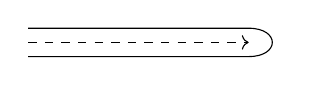
\begin{tikzpicture}
\draw (0,0.18)--(2.8,0.18)..controls (3.2,0.18) and (3.2,-0.18)..(2.8,-0.18)--(0,-0.18);
\draw[dashed,->] (0,0)--(2.8,0);
\end{tikzpicture}
\end{adjustbox}
контур, охват. спектр.
\SourceFigure{GELFAND-P000162}{contour-direction}{Две длинные линии, слева открытые, справа соединены округлым поворотом; внутри пунктир со стрелкой вправо. Утолщение внизу правого поворота: направление обхода не установлено.}
Так для отрицат. степеней. Для полож. степеней умн.
на целую полож. степень.
Надо вычислить $\int Tr\,K_s(x,x)dx$
$K_s(x,x)$ — ядро оператора $A^s$, $\Re s\ll0$.

(i) $s\longrightarrow K_s$ — голом. отобр. области $\Re(ms)<-n-k$
в ядра класса $C^k$ на $M\times M$
(гладкая завис. ядра от $s$)

(ii) $C$ — комп. в $M\times M$, не [зачёркнуто слово; сверху
вставлено «пересек. с»] диагональю, то
\Unclear{GELFAND-P000162}{cancelled-intersection}{Между «не» и «диагональю» густо зачёркнуто слово; выше скобкой вставлено «пересек. с». Под зачёркиванием отдельные петли без уверенного буквального чтения.}
$s\longrightarrow K_s|_C$ продолжается [зачёркнуто] в голом. отобр.
\Unclear{GELFAND-P000162}{cancelled-continuation}{После «продолжается» зачёркнуто короткое слово, похожее на «все» / «всё».}
всей плоскости в $C^\infty(C)$
(по $x$ не аналит., т.к. коэфф. бескон. диффер.)

(iii) для любого $x$ $K_s(x,x)$ — мероморфная ф-я
на всей плоск. с полюсами (простыми) возможно лишь
\begin{gather*}
-\frac{n}{m},\quad\frac{1-n}{m},\quad\frac{2-n}{m},\ldots,
-\frac{1}{m},\quad\frac{1}{m},\quad\frac{2}{m},\ldots
\end{gather*}
$(0\text{ — регул. точка})$
При $s=0$ это не единичн. оператор! ([зачёркнуто] ядро не
$\delta$-ф-я)
\Unclear{GELFAND-P000162}{kernel-cancelled-word}{Перед «ядро не» густо зачёркнуты короткие соединённые штрихи, возможно «это»; буквальное чтение не установлено.}

\begin{gather*}
\text{(iv)}\quad (2\pi)^nK_0(x,x)=\frac{1}{m}
\int_{|\xi'|=1}d\xi'\int_{-\infty}^{0}
b_{-m-n}(x,\xi;\lambda)d\lambda
\end{gather*}
$K_0$ не имеет особенностей в вычисл. через коэфф.
[Под «коэфф.»: «опер. $A$.»]

$A^s$ — псевдодифф. опер. и символ его получается естеств.
образом подстан. символа вместо $A$ в ф-лу для $A^s$.
Индекс — разность двух выраж. типа (iv).

\SourcePage{GELFAND-P000163}{unlabelled}
\underline{Минлос.} \underline{Лекция 3.}
$(\mathcal{Y}_{\Omega,N},H(\alpha,\beta))$
\Unclear{GELFAND-P000163}{configuration-letter}{Первый знак перед $\Omega,N$ каллиграфический: высокий петлевой ствол, левая дуга и правая петля; $\mathcal{Y}$ / $\mathcal{G}$ / иной рукописный знак. Тот же знак далее перед отображением и в распределении.}
Можно ли указать «предельное пр-во», облад. асимпт. св-вами?
Вероятно, да, но док. опять для малой плотности.
Перейдём к неразличимым частицам
\begin{gather*}
\mathcal{Y}'_{\Omega,N}\longrightarrow C_{\Omega,N}
\end{gather*}
[Под $\mathcal{Y}'_{\Omega,N}$: $x_i\ne x_j$]
$C_{\Omega,N}$ — $N$-точечные подмн-ва сосуда.
$H$ можно рассм. на $C$, т.к. она симметрична
Распр. Гиббса переносится
\begin{gather*}
P_{C_{\Omega,N}}(c)=P_{\mathcal{Y}'_{\Omega,N}}(\widetilde c)
\end{gather*}
[Под $\widetilde c$, со стрелкой вверх: «прообраз.»]
* доп. к $\mathcal{Y}'$ имеет меру $0$.

$C_\infty$ — конечные или счётные подмн-ва $R^\nu$
(не имеющие пред. точек), $d\in C_\infty$.
На нём можно задать распред. Гиббса.
\underline{Сначала выделим $\sigma$-алгебру.}
Цилиндрич. мн-во. $U\subset R^\nu$
\begin{gather*}
S_{U,k}\ (d:n(d,U)=k)
\end{gather*}
число точек, попавших в $U$ равно $k$.
Конечн. набор непересек. мн-в
[Конец сокращения «мн-в» переписан густо.]
\begin{gather*}
S_{U_1,U_2,\ldots,U_s;k_1,k_2,\ldots,k_s}
=\{d:n(d,U_1)=k_1,\ldots\}
\end{gather*}
$\sigma$-алг., порожд. этими цилиндрич. множествами.
Обычное распред. Гиббса порожд. меру на этой $\sigma$-алгебре.
Получ. меры удовл. условию равномерного сильного
перемешивания. это предельная мера. Её существование
док. для малых плотностей.
\begin{gather*}
\mu(S_{U_1U_2,k_1k_2})-\mu(S_{U_1,k_1})\mu(S_{U_2,k_2})\longrightarrow0,\\
d(U_1,U_2)\longrightarrow\infty
\end{gather*}
(равном. сильное перемешивание)
равномерно по всем парам $U$

Трудность — есть сущ. на [густо зачёркнуто] цилиндр. мн-вах
\Unclear{GELFAND-P000163}{cancelled-bottom}{После «на» густо зачёркнуто длинное слово с двумя нижними штрихами: «корреляц.» / иное слово; читаемые части не дают уверенного восстановления.}
Это $\longrightarrow$ переформулир. свойств корреляц. ф-й.

\SourcePage{GELFAND-P000164}{26}
\underline{Св-ва, вытек. из этого.}
$1^\circ$. Для почти всех $d$ сущ. средняя плотность —
— следствие теор. Биркгофа и эргодичести меры.

\underline{Предл. Гельфанда}: начать с аксиом о корреляц. функциях.
Как их выделить?
\underline{Термодин. величины.}
\begin{gather*}
\begin{array}{cccc}
E & P & S & F\\
\text{энергия} & \text{давление} & \text{энтропия} & \text{своб. энергия}
\end{array}
\end{gather*}
\begin{gather*}
Z=\frac{1}{N!}\int_{\mathcal{Y}_{\Omega N}}e^{-\beta H(a)}da
\end{gather*}
— нормир. множитель.
\Unclear{GELFAND-P000164}{partition-domain-letter}{Знак области интегрирования совпадает с каллиграфическим петлевым знаком предыдущего кадра: $\mathcal{Y}$ / $\mathcal{G}$ / иной знак; индексы здесь $\Omega N$ без ясно видимой запятой.}
Все они выраж. через $\ln Z$
Будем док., что сущ. $\lim\dfrac{\ln Z}{N}$

\SourcePage{GELFAND-P000165}{27}
$10/\overline{X}$ \underline{Сем. Гельфанда}
\underline{Минлос} \underline{Лекция 4.}
\begin{gather*}
\begin{array}{ccc}
E & P & S\\
\text{энергия} & \text{давление} & \text{энтропия}
\end{array}
\end{gather*}
$(\mathcal{Y},H(a),\beta)$
\Unclear{GELFAND-P000165}{configuration-letter}{В тройке первый знак тот же петлевой каллиграфический знак: $\mathcal{Y}$ / $\mathcal{G}$ / иной знак.}
$1^\circ$. $E=\langle H(a)\rangle$. Для $H(a)=\sum U(|x_i-x_j|)$ была
док. репрезентативность, т.е. $\langle H(a)\rangle\approx Ne$, $e=e(v,\beta)$
[Под $Ne$: $N,\Omega\longrightarrow\infty$]
\Unclear{GELFAND-P000165}{density-variable}{Аргумент в $e(v,\beta)$ написан $v$- / $\nu$-подобно; латинский / греческий знак не различён.}
\begin{gather*}
\langle H(a)\rangle=\frac{\int H(a)e^{-\beta H(a)}da}{Z}
=-\frac{\partial}{\partial\beta}\ln Z
\end{gather*}
$2^\circ$. $p(x)=\tau_1(x)$. $P=\dfrac{1}{S}\int p(x)d\sigma$
(До пред. перехода)
\Unclear{GELFAND-P000165}{pressure-correlation-letter}{Знак с индексом $1$ после $p(x)=$ имеет верхнюю дугу и нижний крючок: $\tau_1$ / $r_1$; он повторяется в скобке ниже.}
Сущ. гипотеза, что $p(x)\longrightarrow const$ в термодин. пред. переходе.
это не следует из ранних гипотез
это $\forall$ конечн. участке)
[Справа: $(\text{что }\tau_1\longrightarrow const,\text{ т.к.}$]
\begin{gather*}
p=\frac{\partial\ln Z}{\partial V};
\end{gather*}
$3^\circ$. Энтропия распр. Гиббса:
$\forall$ распр. $\pi(x)$
\begin{gather*}
S=\int\pi(x)\ln\pi(x)dx;\qquad
\frac{S}{N}=\frac{1}{N}\ln Z-\frac{1}{\beta}
\frac{\partial}{\partial\beta}\frac{\ln Z}{N}
\end{gather*}
Сущ. пред. энтропии на $1$ частицу.

\underline{В. И. Арнольд.} О работах Маслова.
$R^{2n}$ — фазовое пр-во $p_1,\ldots,p_n,q_1,\ldots,q_n$, если введ.
$3$ структуры

1) метрика $p^2+q^2$ и скал. произв. (евкл. структура) $(x,y)$

2) компл. структура $z=p+iq$, $R^{2n}=C^n$, $I$ — опер. умн.
на $i$.

3) симплектич. структура $[x,y]=$ [зачёркнуто] \fbox{$(Ix,y)$}
\Unclear{GELFAND-P000165}{cancelled-symplectic-term}{Перед $(Ix,y)$ густо зачёркнут короткий математический знак / термин; отдельные штрихи не дают уверенного чтения.}
[Под рамкой: «вещ. скал. произв.»; соседняя рамка справа:
«ортог. [переписанное сокращение]», со стрелкой от $I$.]
\Unclear{GELFAND-P000165}{orthogonal-abbreviation}{После «ортог.» сокращение густо переписано: «преобр.» / «произв.» / иное; начало «пр» и нижний штрих видимы.}
это кососим. форма
В механике есть только $3$-я структура в кас. пр-ве.
\Unclear{GELFAND-P000165}{mechanics-space-word}{Перед «пр-ве» сокращение выглядит «кас.» / «касс.» / иной термин; математическое ожидание «фаз.» не подтверждено буквальными штрихами.}
Сохр. этих структур: $O(2n)$, $GL(C,n)$, $Sp(n)$
Легко док., что попарные пересеч. равны тройному (из [3])
\underline{это $U(n)$.}

\underline{Подпр-во $R^n$ наз. Лагранжевым}, если на нём $3$-я
форма $0$ $(IR^n\perp R^n)$. \underline{Напр.}, вещ. и чисто мнимые.
\begin{gather*}
[R^n,R^n]=0
\end{gather*}

\SourcePage{GELFAND-P000166}{unlabelled}
\underline{Пример.} $p=p(q)$ — лагранжево мн-зие
$\Longleftrightarrow\ \exists S(q),\text{ что }p=\dfrac{\partial S(q)}{\partial q}$
$n=1$ — любая кривая — лагр. мн-зие
$n=2$ — не любая.
Лагр. плоск. — вещ. подобные, $U(n)$ действ. транзитивно
$O(n)$ оставл. на месте вещ. плоск.
Лагр. плоскости $\Lambda(n)=U(n)/O(n)$ — лагр. мн-зие Грассмана
(Лагр. плоск. разм. $\leq n$, но здесь только тех разм. $n$)
$M$ — лагранжево мн-зие (кас. пр-во $\forall$ точке лагранжево)
Постр. отобр.
\begin{gather*}
\Lambda(n)\longrightarrow S^1
\end{gather*}
$(det\text{ унит. преобр. }U(n))^2$
с точн. до $O(n)$, $det=\pm1$
$U(n)$ перев. вещ. плоск. в нашу лагранжеву.
\begin{adjustbox}{max width=\linewidth}
\begin{tikzcd}
SO\arrow[r]\arrow[d]&O\arrow[r]\arrow[d]&S^0\arrow[d]\\
SU\arrow[r]\arrow[d]&U\arrow[r,"det"]\arrow[d]&S^1\arrow[d,"z^2"]\\
S\Lambda\arrow[r]&\Lambda\arrow[r,"det^2"]&S^1
\end{tikzcd}
\end{adjustbox}
$S\Lambda$ — слой соотв. расслоения.
Это дифф. расслоений.

$M^n$ — лагр. мн-зие. Есть тангенц. отображение
\begin{gather*}
S^1\overset{\gamma}{\longrightarrow}M^n
\longrightarrow\Lambda(n)\overset{det^2}{\longrightarrow}S^1
\end{gather*}
[Перед $S^1$ густо переписан знак.]
\Unclear{GELFAND-P000166}{curve-quantifier}{Перед цепочкой $S^1\longrightarrow M^n$ густо переписанный знак: $\forall$ / зачёркнутая запись; исходный знак не установлен.}
[Под цепочкой от $M^n$ до $S^1$ проведена длинная черта.]
$M^n\longrightarrow S^1$ определяет кацикл (в обр. сторону)
\Unclear{GELFAND-P000166}{cocycle-word}{Слово после «определяет» выглядит «кацикл» / «коцикл» / «нацикл»; начальная буква и первая гласная не различены уверенно.}
$\gamma$ — кривая в $M^n$
\begin{gather*}
l(\gamma)=\operatorname{deg}(Det^2\circ\tau\circ\gamma),\qquad
l\in H^1(M,Z)
\end{gather*}
\Unclear{GELFAND-P000166}{maslov-class-letter}{Знак перед $(\gamma)$ и перед $\in H^1$ имеет высокий ствол и нижнюю петлю: $l$ / $\ell$ / $\mu$-подобный знак.}
Это индекс Маслова, участв. в ф-лах асимптотики,
в частности, получ. индекс Морса (число сопр. точек на геод.)
Есть другое геометрич. опред. Маслова.

\SourcePage{GELFAND-P000167}{29}
$17/\overline{X}$ \underline{Сем. Гельфанда.}
\underline{Минлос.} \underline{Лекция 5.}
Фазовые переходы.
\underline{И. М. Гельфанд.} \underline{Теор. двойств. Танака — Крейна}
$G$ — кон. группа или компактная.
Даны предст., неприв., конечномерные в пр-вах $A_1,\ldots,A_n$
\begin{gather*}
A_i\otimes A_k\cong\sum A_j
\end{gather*}
(Тенз. произв. разлож. на непривод. представления)
Рассм. $\sum A_j$ (каждое по $1500$ раз)
\begin{gather*}
A_i\otimes A_j\longrightarrow\sum A_j;
\end{gather*}
т.е. есть набор отображений $d_{ij}$ в абстр. модуль.
Если [зачёркнуто; сверху вписано «свойства этих кратностей»], то
группа в конечн. случае восстан., а в комп. нет.
\Unclear{GELFAND-P000167}{cancelled-multiplicities}{После «Если» зачёркнута длинная запись; поверх / сверху вписаны «свойства этих кратностей». Нижние две черты и отдельные нижние штрихи не дают полного чтения отменённой записи.}
Но пусть даны отобр. в прям. сумму $d_{ij}$, тогда
группа уже восстанавливается.
Пусть $\xi_i\in A_i$.
\begin{gather*}
T_i(g)\xi_i\otimes T_k(g)\xi_k
=\sum T_j(g)d^j_{ik}(\xi_i,\xi_k)
\end{gather*}
Напишем вместо $T_i(g)$ любые $C_i$ — лин. преобр.
[Густо переписано начало:] Пусть верна ф-ла:
\begin{gather*}
C_i\xi_i\otimes C_k\xi_k=\sum C_jd^j_{ik}(\xi_i,\xi_k)
\end{gather*}
У этого ур-я есть решения $C_i=T_i(g)$.
Тогда $C_i=T_i(g)$. Итак, все решения этих ур-й
будут $T_i(g)$ и всё восстанавл. по $d^j_{ik}$.
Есть обобщение на $SL(2,R)$.

\underline{Nirenberg.}
\underline{Varadhan.}
\begin{gather*}
\frac{\partial u}{\partial t}=\sum a^{ij}(x)u_{x^ix^j};\qquad
u(x,0)=\delta(x-y)
\end{gather*}
Изуч. поведение фунд. решения.
\begin{adjustbox}{max width=\linewidth}
\begin{tikzpicture}
\draw[->] (0,0)--(0,0.7) node[above]{$t$};
\draw[->] (0,0)--(0.8,0) node[below]{$x$};
\draw[->] (0,0)--(-0.5,-0.5);
\end{tikzpicture}
\end{adjustbox}
Тогда
\begin{gather*}
u(x)=e^{-\left(\frac{g(x,y)}{t}+o(\frac{1}{t})\right)},\quad t\longrightarrow0
\end{gather*}
первый член разл. по $x$.
Для теплопр. $u=C\dfrac{e^{-\frac{(x-y)^2}{4t}}}{t^{n/2}}$
\begin{gather*}
g(x,y)=d^2(x,y)
\end{gather*}
$d(x,y)$ [зачёркнуто] — расст. по геодезическим
$(t^{n/2}\text{ вход. в }o(\frac{1}{t}))$
в метрике, порожд. $a^{ij}$.
\Unclear{GELFAND-P000167}{cancelled-distance}{После $d(x,y)$ густо зачёркнут термин; буквальные внутренние штрихи перекрыты.}
Ещё эллипт. соб. знач. опер. Лапласа в области в том же духе.

\SourcePage{GELFAND-P000168}{unlabelled}
$24/\overline{X}$. \underline{Сем.} \underline{Гельфанда}
\underline{Вишик}. \underline{Лекция 1.}
I. Опр-ё. Кона-Ниренберга.
II. Теор. об ограниченности.
\underline{Проф. Лосж.} Об ур-и Штурма-Лиувилля.
\Unclear{GELFAND-P000168}{professor-name}{Фамилия после «Проф.» выглядит «Лосж.» / «Лосх.» / «Лорч.»; средние и конечные буквы соединены и пересечены подчёркиванием.}

$31/\overline{X}$ \underline{Сем. Гельфанда.}
\underline{Вишик}. \underline{Лекция 2.}
\begin{gather*}
\sigma(A)=a(x,\xi)\longleftrightarrow A\\
A.Bu=C_0u+\ldots+C_{s-1}u+T_su,
\end{gather*}
где
\begin{gather*}
\sigma(C_k)=\sum_{|\alpha|=k}\frac{1}{\alpha!}
\partial^\alpha a(x,\xi)D^\alpha b(x,\xi)\\
\partial^\alpha=\frac{\partial^{|\alpha|}}{\partial\xi^\alpha},
\qquad D^\alpha=\left(\frac{1}{i}\frac{\partial}{\partial x}\right)^\alpha\\
\sigma(C_0)=a(x,\xi)b(x,\xi)
\end{gather*}
[Под $a(x,\xi)b(x,\xi)$ фигурная черта с подписью $\sigma+\lambda$.]
$T_s$ — опер. порядка $\sigma+\lambda-s$.
\begin{gather*}
\zeta(\xi)a(x,\xi)=h(x,\xi),\qquad
\zeta(\xi)b(x,\xi)=g(x,\xi)\\
\widetilde{Au}(\xi)=(2\pi)^{-n/2}
\int\widetilde h(\xi-\eta,\eta)\widetilde u(\eta)d\eta\\
\widetilde{Bu}(\eta)=(2\pi)^{-n/2}
\int\widetilde g(\eta-\tau,\tau)\widetilde u(\tau)d\tau\\
\widetilde{A.Bu}(\xi)=(2\pi)^{-n/2}
\int\widetilde h(\xi-\eta,\eta)\widetilde{Bu}(\eta)d\eta=\\
=\ldots\int\widetilde h(\xi-\eta,\eta)d\eta
\int\widetilde g(\eta-\tau,\tau)\widetilde u(\tau)d\tau=\\
=\ldots\int\left(\int\widetilde h(\xi-\eta,\eta)
\widetilde g(\eta-\tau,\tau)d\eta\right)\widetilde u(\tau)d\tau
\end{gather*}
Разложим $\widetilde h$ по ф-ле Тейлора при $\eta=\tau$
\begin{gather*}
\widetilde h(\xi-\eta,\eta)=
\sum_{|\alpha|\leq s-1}\frac{1}{\alpha!}
\partial^\alpha\widetilde h(\xi-\eta,\tau)(\eta-\tau)^\alpha
+h_s(\xi-\eta,\eta,\tau)
\end{gather*}

\SourcePage{GELFAND-P000169}{30}
\begin{gather*}
\int\widetilde h(\xi-\eta,\eta)\widetilde g(\eta-\tau,\tau)d\eta
=\int\widetilde h(\xi-\eta,\tau)\widetilde g(\eta-\tau,\tau)d\eta+\\
+\sum\frac{1}{\alpha!}\int\partial^\alpha\widetilde h(\xi-\eta,\tau)
(\eta-\tau)^\alpha\widetilde g(\eta-\tau,\tau)d\eta
\end{gather*}
[Во втором аргументе $\widetilde g$ первого правого интеграла переписан маленький знак перед $\tau$.]
\Unclear{GELFAND-P000169}{overwritten-g-argument}{В первом правом интеграле между $\eta-\tau,$ и последним $\tau$ небольшой густой переписанный знак; возможная отменённая $\xi$ / иной знак не установлен.}
1-я свёртка соотв. произведению $h(x,\tau)g(x,\tau)$
Отсюда всё получается.
\underline{Опред.}
\begin{gather*}
\tau_0,\tau_1,\ldots,\tau_k,\ldots\searrow-\infty\\
A_0,A_1,\ldots,A_k,\ldots
\end{gather*}
$A_i$ однор. пор. $\tau_i$ с символами $a_i(x,\xi)$
\begin{gather*}
A\sim\sum_{k=0}^{\infty}A_k
\end{gather*}
(Заранее $A_i:S\longrightarrow S$)
\begin{gather*}
A-\sum_{k=0}^{N}A_k=T_{N+1}\quad\text{— опер. порядка }<\tau_N.
\end{gather*}
Символ [зачёркнуто $\sigma(A)$-подобное] форм. сумма
\begin{gather*}
\sum_{k=0}^{\infty}a_k(x,\xi)=\sigma(A)
\end{gather*}
\Unclear{GELFAND-P000169}{cancelled-symbol}{После «Символ» зачёркнута формула, похожая на $\sigma(A)$; густые штрихи внутри скобок оставляют чтение неоднозначным.}
Символ $0$ — $A\in\mathcal{L}_{-\infty}$ (порядок $-\infty$)
\Unclear{GELFAND-P000169}{operator-class-letter}{Каллиграфическая буква перед $-\infty$ имеет высокий ствол с верхней и нижней петлями: $\mathcal{L}$ / $\mathcal{Y}$ / иной рукописный знак.}
\underline{Теорема}: символ опер. опред. однозначно.
$\forall$ [зачёркнуто «опер. сущ.»-подобное] символу сущ. оператор.
\Unclear{GELFAND-P000169}{cancelled-operator}{После $\forall$ зачёркнуты два сокращения: «опер. сущ.» / иная запись; видны нижние штрихи и соединяющая длинная черта.}
Псевдодифф. опер. образуют алгебру.
\begin{gather*}
\sigma(A.B)=\sum\frac{1}{\alpha!}
\partial^\alpha\sigma(A)D^\alpha\sigma(B)
\end{gather*}

\underline{О. А. Олейник.}
\underline{Одна частная} зад. механики.
Вязкие жидк. $u,v$ — скор. (плоская). Ур-я Навье-Стокса.
\begin{gather*}
\left\{\begin{aligned}
\frac{\partial u}{\partial t}+u\frac{\partial u}{\partial x}
+v\frac{\partial u}{\partial y}
&=-\frac{1}{\rho}\frac{\partial p}{\partial x}+\nu\Delta u\\
\frac{\partial v}{\partial t}+u\frac{\partial v}{\partial x}
+v\frac{\partial v}{\partial y}
&=-\frac{1}{\rho}\frac{\partial p}{\partial y}+\nu\Delta v\\
\frac{\partial u}{\partial x}+\frac{\partial v}{\partial y}&=0
\end{aligned}\right.
\end{gather*}
$\nu$ — вязкость (малая)
$\nu=0$ — ур-я Эйлера (идеальная жидкость).
Даже для малого $\nu$ нельзя зачёркивать эти члены (Прандтль)
Идеальн. жидк.: гран. усл. — норм. компон. скор. $=0$
вязк. обе комп. $=0$ (прилипание)
\SourceFigure{GELFAND-P000169}{flow-sketch}{Слева у граничных условий открытая слева дуга, выпуклая вправо. Над и под дугой короткие штрихи и стрелки, направленные вправо; справа несколько отдельных штрихов. Подписей нет; точные направления всех коротких штрихов не установлены.}
Всегда есть узкие окр., где сильно отлип.
\Unclear{GELFAND-P000169}{last-word}{Последнее сокращение читается «отлип.» / «отлич.» / иной конец; видимые начальные буквы «от», далее соединённые штрихи.}
\SourcePage{GELFAND-P000170}{unlabelled}
\SourceFigure{GELFAND-P000170}{boundary-geometry}{Вверху слева незамкнутая закруглённая справа линия; у её верхней ветви стрелка вправо с $u$, из той же области стрелка вверх с $v$. Точное положение нормали и касательной дано только рисунком.}
$v$ не мен. (гран. усл. сохр.)
$u$ мен. сильно.
\underline{Остаются ур-я Прандтля:}
\begin{equation*}
\left\{\begin{aligned}
\frac{\partial u}{\partial t}+u\frac{\partial u}{\partial x}+v\frac{\partial u}{\partial y}&=-\frac1\rho\frac{\partial p}{\partial x}+\nu\frac{\partial^2u}{\partial y^2},\\
\frac{\partial u}{\partial x}+\frac{\partial v}{\partial y}&=0.
\end{aligned}\right.
\end{equation*}
[Между строками системы зачёркнуто $\frac{\partial p}{\partial y}=0$.]
$p$ по нормали не мен. и счит., что это изв. ф-я,
получ. из ур-й ид. жидк. $p=p(t,x)$.
[Слева оси: $y$ вверх, $x$ вправо; под положительной полуосью $x$ косая штриховка.]
\begin{equation*}
u|_{y=0}=0,\qquad v|_{y=0}=0,\qquad u|_{x=0}=u_0(x).
\end{equation*}
\Unclear{GELFAND-P000170}{boundary-conditions}{В третьем условии нижняя буква выглядит как $x$: $u|_{x=0}=u_0(x)$; $x$ / $y$-подобный пересекающийся знак.}
\begin{equation*}u(t,x,y)=U(t,x)\qquad y\longrightarrow\infty.\end{equation*}
\begin{equation*}
\left\{\begin{aligned}
\frac{\partial u}{\partial t}+u\frac{\partial u}{\partial x}+v\frac{\partial u}{\partial y}&=\nu\frac{\partial^2u}{\partial y^2}-\frac1\rho\frac{\partial p(t,x)}{\partial x},\\
\frac{\partial u}{\partial x}+\frac{\partial v}{\partial y}&=0.
\end{aligned}\right.
\end{equation*}
\begin{gather*}
u|_{y=0}=0,\qquad v|_{y=0}=v_0(x,t),\qquad u|_{x=0}=u_0(x),\\
u|_{t=0}=u_0(x,t),\qquad \lim_{y\to+\infty}u(t,x,y)=U(t,x).
\end{gather*}
\Unclear{GELFAND-P000170}{initial-conditions}{В условии при $t=0$ справа написано $u_0(x,t)$; второй аргумент выглядит как $t$, хотя возможна $y$-подобная нижняя петля.}
Реш. единств., если оно существует.
Можно док., что сущ. для промеж. $0\le t\le T$ для всего
обтек. тела (отрыв может быть, но не мгновенно).
Вблизи нач. обтекания сущ. $\forall t$.
\begin{equation*}\frac{\partial p}{\partial x}\le0.\end{equation*}
Решение всегда устойчиво, если оно сущ. и явл. наст.
погр. слоем.
\Unclear{GELFAND-P000170}{last-abbreviations}{Последнее сокращение первой строки: «наст.» / «насл.»; начальные и средние соединённые штрихи плотные.}

\SourcePage{GELFAND-P000171}{unlabelled}
\underline{14/XI. Сем. Гельфанда.}
\underline{Агранович. Лекция 3 по псевдодифф. операторам.}
\underline{Проблемы дифф. геом.}
1. Есть полное рим. мн-зие отриц. кривизны.
$f\in C_0^\infty(\Omega)$, дан шар $B$ и $\int$ по любой сфере,
содержащей $B$, $=0$. Док., что $f=0$ вне $B$.
(Хелгасон) Для пост. крив. сделано. (Хелгасон)
\Unclear{GELFAND-P000171}{helgason-name}{Фамилия в обеих скобках: «Хелгасон» / «Хельгасон»; короткие соединённые штрихи после «Хе» не вполне раздельны.}
2. \Unclear{GELFAND-P000171}{cancelled-calabi-star}{Перед подчёркнутым Calabi густо зачёркнут небольшой знак с вертикальным штрихом и нижней петлёй; звёздочка / отменённая буква.}
\underline{Calabi}
$U(x)$ — вып. ф-я в $R^n$.
\begin{equation*}\det\left(\frac{\partial^2u}{\partial x_i\partial x_j}\right)=1.\end{equation*}
Док., что $U$ — многочлен 2-й степени.
Доказано для $n=2$ и для $n\le5$ Calabi.
3. $u(x)\in C^\infty(R^n)$, удовл. след. условию:
(Calabi)
\Unclear{GELFAND-P000171}{minimal-equations}{Первая формула густо зачёркнута: видны $(1+\sum u_{x_i}^{2})$, несколько наложенных штрихов, $(\sum u_{x_jj}''{}^{\,2})-\sum u_{x_i}''$-подобное начало конца; дальнейшие индексы отменённой строки не отделяются уверенно. В чистой строке после двойного штриха у $u_{x_jj}$ виден отдельный поднятый $2$; двойное $j$ / сжатое $x_jx_j$ и этот $2$ сохранены без исправления.}
\begin{equation*}
\left(1+\sum u_{x_i}^{2}\right)\left(\sum u_{x_jj}''{}^{\,2}\right)
-\sum u_{x_ix_j}''u_{x_i}'u_{x_j}'=0.
\end{equation*}
Верно ли, что $u$ линейна?
(Это ур-я мин. поверхн.)
Сделано. (у De Giorgi есть ссылка)
\Unclear{GELFAND-P000171}{degiorgi-name}{Латинское имя в скобке выглядит как De Giorgi / De Gicrigi / De Giccilgi; средние буквы слитны.}
4. $M$ — комп. рим. мн-зие.
\begin{equation*}
L_1^2(M),\quad \langle\varphi,\psi\rangle=\int_M\varphi\psi\,dx+\int\langle d\varphi,d\psi\rangle\,dx.
\end{equation*}

\SourcePage{GELFAND-P000172}{33}
\begin{equation*}D(\varphi)=\frac12\int_M|d\varphi|^2\,dx\quad\text{— пр-во }D^1.\end{equation*}
\Unclear{GELFAND-P000172}{dirichlet-link}{Перед «пр-во $D^1$» густой горизонтальный штрих: тире / стрелка вправо; левый конец частично наложен. Направление не установлено.}
\begin{gather*}(L_1^2(M),D)\\(L_1^2(M'),D').\end{gather*}
Есть изометрия $L_1^2(M)$, индуцир. диффеом. $M$ и $M'$.
Док., что $M'$ и $M$ изометричны.
Инварианты — соб. знач. опер. Лапласа.
\Unclear{GELFAND-P000172}{cancelled-number-word}{Над номером 5 зачёркнуто короткое «Ер» / «Ор»-подобное слово.}
5. $M$ — $n$-мерн. комп. неприв. симм. пр-во.
$\Delta$ — опер. Лапласа.
$V$ — соб. пр-во, отвеч. наименьшему соб. знач. $\ne0$.
\begin{equation*}\varphi:M\longrightarrow V^*.\end{equation*}
\Unclear{GELFAND-P000172}{compact-line}{Строка под отображением: «Если не компактно.» / «Если … компактно.»; короткие штрихи перед «компактно» бледны.}
6. $M$ — полное некомп. рим. мн-зие (3-мерн.) полож. кривизны
(тензор Ricci $>0$).
Будет ли $V$ здесь уходить в $\infty$.
(Для 2-мерн. мн. док. Кн-Фоссеном)
\Unclear{GELFAND-P000172}{cohn-vossen}{Фамилия: «Кн-Фоссеном» / «Кон-Фоссеном»-подобные слитные штрихи с возможным вторым «с»; каталожное написание не подставлено.}
7. $M$ — комп. $n$-мерное мн-зие.
Сущ. ли $\infty$-много
\Unclear{GELFAND-P000172}{geodesic-cancellation}{Перед «пересек.» зачёркнуто «пар» / короткое слово с нижним штрихом.}
пересек. геодезических.
\Unclear{GELFAND-P000172}{geodesic-parenthesis}{Скобка: «(фактически различных)» / слитное длинное слово перед «различных».}
\Unclear{GELFAND-P000172}{eighth-numeral}{Следующий номер выглядит как «3.» / «8.»: сверху маленькая петля, снизу открытая дуга.}
$M$ — комп. односвязное рим. мн-зие, в к-ром все
геод. замкнуты и имеют одинак. длину. Док., что
оно диффеом. симм. пр-ву
\Unclear{GELFAND-P000172}{cancelled-rank}{Перед «1-го типа» зачёркнут $\rho=$ / $p=$-подобный знак с продолжением.}
1-го типа. (?)
Есть аналит. мн-зие, диффеом. сфере, но не изометр.
(Bott). Bott док., что та же когом. структура.
9. На любом ли комп. $M^3$ сущ. контактная структура?

\SourcePage{GELFAND-P000173}{unlabelled}
\underline{21/XI. Сем. Гельфанда.}
\underline{Арнольд.}
\underline{Лекция 1.}
\underline{Теория особенностей дифф. отображений.}
\begin{equation*}f:M^m\longrightarrow N^n.\end{equation*}
$y=x^2$.
\SourceFigure{GELFAND-P000173}{function-graphs}{У $y=x^2$ маленькая U-образная линия над горизонталью с вертикальным штрихом у нижней точки. Ниже у $y=x^3$ оси со стрелками вверх и вправо и S-подобная линия, идущая снизу слева вверх вправо. Буквенных меток на самих осях нет; точные касания при плотном пересечении не устанавливаются.}
Устойч.
\Incomplete{GELFAND-P000173}{stable-cancellation}{Между «Устойч.» и «особ.» густо зачёркнуто короткое слово; начало и петля последней буквы не отделяются уверенно.}
особ.
(у близкого дифф. отобр. прив. к тому же виду)
$y=x^3$. Неуст. особ.
\begin{center}
\begin{adjustbox}{max width=\linewidth}
\begin{tikzcd}
M^m\arrow[r,"f"]\arrow[d,"h"']&N^n\arrow[d,"k"]\\
M^m\arrow[r,"g"']&N^n
\end{tikzcd}
\end{adjustbox}
\end{center}
\underline{Топ. уст.} $\exists$ гомеом. $h$ и $k$.
(дифф.) $\downarrow$ Дифф. устойч.
Устойчивость в $0$ — на окрестностях то же самое.
(ростки отображений).
(Можно так изм. мн-зия, чтобы отобр. задавалось
теми же ф-лами)
\Unclear{GELFAND-P000173}{minimum-maximum}{Начало строки перед «— устойчив»: Rang max / Ring max / min max; первое слово имеет высокий петлеобразный начальный знак и нисходящий последний штрих.}
— устойчив (невыр. ф-я).
Лемма Морса — невыр. квадр. форма ($R^n\to R^1$ устойч.)
Теор. Уитни $M^2\to N^2$ тоже исчерп. рез.
\underline{Морс} $M$ — комп. 1) уст. отобр. $M\to R^1$ обр. открытое
всюду плотное мн-во.
2) Усл. на устойчивость (необх. и дост.):

\SourcePage{GELFAND-P000174}{unlabelled}
\underline{M.1} Все крит.
\Unclear{GELFAND-P000174}{critical-cancellation}{Перед «точки» густо зачёркнуто слово с $з$-подобным началом: «знач.» / наложенные короткие штрихи.}
точки невырожд.
\underline{M.2} Все крит. значения различны.
3) \underline{лок. утв.} лок. устойчивость $\Longleftrightarrow$ можно выбр.
коорд. так, что запис. ф-ции (один из способов)
\begin{gather*}y=x_1\\y=x_1^2+\ldots+x_k^2-x_{k+1}^2-\ldots-x_m^2.\end{gather*}
(уст. и топ. и дифф.)
\underline{Теор. Уитни.}
1) Уст. отобр. плотны.
2) $f:M^2\to R^2$ устойч. $\Longleftrightarrow$
$\Longleftrightarrow$
\Unclear{GELFAND-P000174}{whitney-labels}{Первый подчёркнутый номер: W1 / M1; два угловых штриха сильно наложены. Следующий номер читается W2.}
все крит. точки невыр.
\underline{W2} крит. знач. трансверсальны (образы складок)
3) \underline{Устойч. в д. точке} $\Longleftrightarrow$ отобр. запис. одной из ф-л:
\begin{align*}
1.\quad&y_1=x_1,\quad y_2=x_2,\\
2.\quad&y_1=x_1,\quad y_2=x_2^2\quad\text{(складки)},\\
3.\quad&y_1=x_1,\quad y_2=x_1x_2+x_2^3.
\end{align*}
\SourceFigure{GELFAND-P000174}{projection-geometry}{Слева шарообразный контур над параллелограммом; поперёк контура эллипс с пунктирной верхней дугой, на плоскости под ним отдельная незамкнутая овальная линия. Подписей и явной соединяющей стрелки нет; точная проекция не дорисована.}
2. — точки складки, это кривые, где якобиан $=0$.
\underline{W2} — образы складок
\Unclear{GELFAND-P000174}{whitney-negation}{Перед «пересек.» зачёркнуто «не» / плотный короткий горизонтально перечёркнутый знак.}
пересек. трансверс.
\underline{W3} — образы сборок различны.
3.
\SourceFigure{GELFAND-P000174}{cusp-diagrams}{Слева оси $x_1$ вправо, $x_2$ вверх и закруглённая линия с вершиной у пересечения, ветви идут влево вверх и влево вниз; на ветвях короткие чёрточки. К нижней ветви подходит изогнутая выноска «сборки». Справа оси $y_1$ вправо и $y_2$ вверх, две толстые ветви из левой верхней и левой нижней области сходятся в пересечении осей. Расположение чёрточек и плотного касания требует исходного рисунка.}
[Ниже слева оси со стрелками вверх и вправо и две почти вертикальные линии справа от вертикальной оси.]
При $x_1>0$ на верт. прямых монот.
\begin{equation*}x_1=\operatorname{const}\Rightarrow y_1=\operatorname{const}.\end{equation*}
При $x_1<0$ будет
\SourceFigure{GELFAND-P000174}{cubic-graph}{После «будет» горизонталь и кривая: сверху слева вниз через горизонталь, затем маленькая впадина, подъём над горизонталью и снова спад ниже неё справа. Букв и стрелок нет; форма сохраняется по источнику без координатного восстановления.}
Чёрточки на параб. — напр. вырождения.
Сборка — где напр. вырожд. касается параболы.

\SourcePage{GELFAND-P000175}{36}
Устойчивость — корни должны слиться (переход от
немонот. отобр. к монотонному) Это нечётный порядок.
\begin{equation*}z\longrightarrow z^2.\end{equation*}
[Под отображением волнистое подчёркивание.]
Неустойч. особенность.
Исканое возмущение: $z\to z^2+\varepsilon\bar z$.
\Unclear{GELFAND-P000175}{complex-perturbation}{Первое слово строки: «Исканое» / «Искомое»-подобные соединённые штрихи; над последним $z$ горизонтальная черта, ниже справа отдельные наклонные штрихи прилегающего рисунка.}
\SourceFigure{GELFAND-P000175}{three-cusp-figures}{Слева три вложенные окружности: точка в центре, на средней окружности три густые точки, к нижней выноска «Особ.». Рядом три петлеобразные лепестка с пересечениями в центре, густые точки в верхнем, левом нижнем и правом нижнем направлениях. Справа большой рисунок: несколько треугольных с вогнутыми сторонами контуров, верхняя петля, внешние пунктирные дуги и наклонные штрихи у нижних вершин; точная связность наложенных линий не устанавливается. Подпись «(Куда переш. окружности?)».}
Большие окр. делают 2 оборота (трилистн. узел)
\Unclear{GELFAND-P000175}{circle-caption}{Сокращение в скобке: «трилистн.» / «трилистн»-подобное начертание, последняя буква перед точкой соединена со штрихом «узел».}
До разм. 5-6 классифик. есть.
\underline{Теорема 1} (Том)
При отобр. $R^9\to R^9$ (и больше) всюду плотность
устойч. ростков не имеет места.
(с $R^9$ есть инварианты дифферен. и они мен.)
Нач. с 12, инвар. беск. много.
\Unclear{GELFAND-P000175}{thom-claims}{В скобке «инварианты дифферен. и они мен.»; сокращённое «мен.» / «мен»-подобное окончание не расширено. В следующей строке виден 12, подчёркнут волнистой скобкой.}
Том:
\underline{Теорема 2.}
Сущ. дискр. топ. классифик. существует!!!
(Как она выглядит — неизвестно)
(Если из пр-ва всех отобр. выкинуть $A_\infty$ — беск.
коразм.
\begin{equation*}A=\bigcup_{\gamma\in\Gamma}A_\gamma+A_\infty.\end{equation*}
$\Gamma$ — счётное мн-во.
Каждое $A_\gamma$ — конечн. коразм.; все ростки $A_\gamma$ топ.
экв. друг другу, при разных $A_\gamma$ не сов.
\Unclear{GELFAND-P000175}{topological-insert}{Справа в скобках: «(в $A$ струй. алг. мн-зия при топ.», затем ниже «топ. устойч.»; наклонная выноска от строки конечной коразмерности к этой приписке. Буквы «струй.» / «структ.» и короткое «топ.» / «том.» не отделяются уверенно; видимая открытая скобка не дополнена.}
\Unclear{GELFAND-P000175}{constant-map}{Скобка внизу: «(Прямая перех. в точку — отобр. вх. в $A_\infty$)» / «… вл. в $A_\infty$»; «перех.» и «в точку» подчёркнуты.}
[Горизонтальная черта.]
\begin{equation*}f:M^m\longrightarrow N^n\qquad\text{росток отобр.}\end{equation*}
\underline{Струя} пор. $k$: $j_0^k(f)$ — класс эквив. отобр., имеющих
касание пор. $k$ в точке $0$.
\begin{equation*}f(x)-g(x)=o(x^k)\qquad\text{в точке }0.\end{equation*}
\Unclear{GELFAND-P000175}{jet-remainder}{Последний знак остатка: маленькая овальная $o$ / $O$; аргумент выглядит $x^k$, без видимых модульных черт. Нижняя строка у границы кадра учтена без добавленного продолжения.}

\SourcePage{GELFAND-P000176}{unlabelled}
\underline{Струи} \underline{порядка} $0$ — образ точки.
[Во второй строке под «Струи» знак повторения.]
$1$ — образ и его дифференциал.
\begin{equation*}j_0^k(f)\qquad\text{опред. инвариантно}\quad\text{(опр. инвар.)}\end{equation*}
Струи фикс. пор. — алг. мн-зие (в координатах —
— ряды Тейлора). Пучок струй отобр. из $M$ в $N$
\begin{equation*}J^k(M,N)\quad\text{— пучок над }M.\end{equation*}
Для $N=R^n$ это вект. пучок.
(С естеств. топ., дифф. и алг. структурой)
\begin{equation*}R^n\longrightarrow R^1.\end{equation*}
\Unclear{GELFAND-P000176}{jet-fibre-glyph}{Начальный знак в строке перед «— кольцо срезанных полиномов»: $J_x^k(R^n,R^1)$ / $j_x^k(R^n,R^1)$; через вертикальный штрих начальной буквы несколько коротких поперечных штрихов.}
— кольцо срезанных полиномов
\begin{gather*}R[x_1,\ldots,x_n]\\j_x^k(f)=j_x^k(n,1)\\(f:R^n\to R^1).\end{gather*}
\begin{equation*}j_0^k(n,1)=R[x_1,\ldots,x_n]/M^k\qquad(M=(x_1,\ldots,x_n)).\end{equation*}
\Unclear{GELFAND-P000176}{jet-ring-power}{В знаменателе $M^k$; у $M$ длинная опущенная левая ножка, рядом верхний $k$. Отдельного $+1$ в показателе не видно; возможное слияние коротких штрихов не восстановлено.}
\underline{Мн-зие} конечной коразм. $e$ в $J^k(M,N)$ в точке,
если оно зад. $e$ ур-ями.
\underline{Естеств. отобр.:}
\begin{equation*}f\overset{j}{\longrightarrow}j_x^k(f).\end{equation*}
\Unclear{GELFAND-P000176}{jet-map-mark}{Справа от отображения отдельный вертикальный извилистый знак: $\xi$ / росчерк с тремя выступами. Присоединение к формуле не показано.}
\Incomplete{GELFAND-P000176}{admissible-cancellation}{Слева перед строкой густо зачёркнуто короткое слово с петлями, под ним буквы не восстанавливаются. Над следующим зачёркнутым «Доп.» / «Это»-подобным словом вставлено подчёркнутое «Допустимое». Далее подчёркнуто «мн-во:».}
прообразы мн-в конечной коразм.
в одном из $J$.
Рассм. $f:M^m\longrightarrow N^n$.
\begin{gather*}x\in\Sigma^i(f),\quad\text{если}\\\dim\operatorname{Ker}df\big|_x=i.\end{gather*}
\SourceFigure{GELFAND-P000176}{parabola-sets}{Слева горизонтальная и вертикальная линии, густая точка у пересечения; закруглённая кривая с вершиной в этой точке, две ветви уходят влево вверх и влево вниз. Явных стрелок и букв на осях нет; линия нижней ветви и границы густой точки остаются по источнику.}
$\Sigma^0$ — все т. без параб.
$\Sigma^1$ — вся парабола.
\underline{Теорема.}
Плотно мн-во всех отобр., где $\Sigma^i$ — мн-зия, причём
\begin{equation*}\operatorname{codim}\Sigma^i=\operatorname{corang}_x\cdot\operatorname{corang}_y.\end{equation*}
\Unclear{GELFAND-P000176}{rank-product}{Под формулой слева «$(i=)(m-r)$», затем густо зачёркнутый горизонтальный соединяющий штрих с дугой справа; отдельно подчёркнуто $n-r$. Между двумя множителями не добавлен отсутствующий ясный знак. Под $m$ два коротких жирных штриха у нижней границы кадра.}
$(r$ — ранг дифф.)
(Это ф-ла, впрочем, очевидна.)

\SourcePage{GELFAND-P000177}{37}
$z\longrightarrow z^2$ уже неуст.
Условие на $\Sigma^i$ — алгебр. подмн. в $J$ — нужные
коразм. (миноры $=0$).
В $J^1(M,N)$ опред. мн-зия $\Sigma^1,\Sigma^2,\ldots$ только
по росткам.
Реальное отобр. $\Rightarrow$ сечение.
\Unclear{GELFAND-P000177}{corank-parenthesis}{Подчёркнутое и переписанное начало скобки: «Коранг» / «Коразм.», затем «— коразм. образа $d..$)»; после $d$ два маленьких раздельных штриха.}
\begin{center}
\begin{adjustbox}{max width=\linewidth}
\begin{tikzcd}
A\arrow[r,"f"] & B & C\arrow[l,"g"]
\end{tikzcd}
\end{adjustbox}
\end{center}
$f,g$ трансверсальны, если $\forall a\in f^{-1}(b),c\in g^{-1}(b)$
в точке $b\in B$
вып. соотн:
\begin{equation*}f_*TA_a+g_*TC_c=TB_b\qquad\text{(пересек. могут).}\end{equation*}
2 прямые в $R^3$ не трансверс. ни в 1 точке (если
они пересек.) (могут пересекаться).
Если отобр. трансверс. подмн-зию,
$(g$ — вложение $C\subset B)$,
то прообраз мн-зия — мн-зие.
Codim его такая же
\begin{equation*}\operatorname{codim}f^{-1}C\big|_A=\operatorname{codim}C\big|_B.\end{equation*}
Если $f:M\longrightarrow N$ трансверс. к $\Sigma^i$, то всё хорошо.
Можно пошевелить $\forall$ отображение.
\underline{Дальнейшая классифик.}
\begin{equation*}\Sigma^i f\subset M,\qquad f:M\longrightarrow N.\end{equation*}
Предполож., что сечение, опр. отобр. $f$, трансверс.
$\Sigma^i$ в струях.
В $\forall$ точке $x\longrightarrow J$. Оно трансверс. отобр. $\Sigma^i$
(без $f$) в $J$.
Возник. отобр. $f|\Sigma^i f\subset M$.
[Из-под правой части этой строки наклонная стрелка вниз вправо к $N$.]
\SourceFigure{GELFAND-P000177}{bottom-curve}{Внизу слева закруглённая кривая с правой вершиной и двумя ветвями, уходящими влево; на верхней и нижней ветвях поперечные чёрточки. Осей и подписи нет, длина и размещение чёрточек не восстановлены.}

\SourcePage{GELFAND-P000178}{unlabelled}
К нему прим. та же классифик.:
\begin{gather*}\Sigma^j f|\Sigma^i f\\x\in\Sigma^{ij}(f)\quad\text{— подмн-зие (Boardman 1965)}.\end{gather*}
(Можно пошевелить) $\forall$ числа индексов.
\underline{Теор.}
1. $\forall k$ в $J^k(M,N)$ опред. алгебр. подмн-зия
\begin{equation*}\Sigma^I\qquad I=(i_1,\ldots,i_k)\quad\text{(независ. от }f\text{)}.\end{equation*}
Codim есть $\nu(I)$ посчитана (сложная).
2. Всякое отобр. аппрокс. отобр., трансв. всем этим
\begin{equation*}\Sigma^I(f).\end{equation*}
\underline{Классифик.} $\Sigma^{110}$ и т.д.
Это не полный набор инвар. (впервые в $R^4$),
\Unclear{GELFAND-P000178}{rank-last-line}{После скобки «но» / «по», ниже «падению рангов не различаются.»; первый соединённый знак после запятой состоит из двух восходящих ножек. «не полный» написано раздельно; утверждение не дополнено недостающим подлежащим.}

\SourcePage{GELFAND-P000179}{unlabelled}
\underline{28/XI.} \underline{Сем.} \underline{Гельфанда.}
[\underline{Арнольд}
\Unclear{GELFAND-P000179}{header-cancellation}{После фамилии в квадратных скобках густо зачёркнуты два-три знака: «УР» / «Ч»-подобные наложенные штрихи; исходное слово не установлено.}
]
\begin{equation*}f:M^m\longrightarrow N^n.\end{equation*}
\begin{equation*}\Sigma^i(f)=\{x\in M^m:\dim\ker df_x=i\}\quad\text{— подмн-во}.\end{equation*}
если оно мн-зие, то
\begin{equation*}\Sigma^{ij}(f)=\Sigma^j\Sigma^i(f)=\Sigma^j(f|\Sigma^i f)\quad\text{— наивное опред. Тома}.\end{equation*}
(забыть)
$\forall$ мультииндекса $i_1,i_2,\ldots,i_k=I$ определено
\begin{equation*}\Sigma^I(f),\end{equation*}
если всё время получ. мн-зия.
Должно быть
\begin{equation*}i_1\ge i_2\ge\ldots\end{equation*}
\begin{equation*}K_1=\operatorname{Ker}df_x,\qquad K_2\subset K_1\quad\text{— след. ядро на послед.}\end{equation*}
подмн-зии.
Есть независ. от отобр. подмн-во $\Sigma^I\subset J^k(M,N)$
(строится)
[Слева вдоль следующих двух строк две вертикальные черты.]
$A$ — кольцо ф-й на мн-зии с коорд. сист. $x_1,\ldots,x_m$
$B\longrightarrow$ идеал в $A$.
Новый идеал — якобиево расширение $B$ пор. $k$ $\Delta_k(B)$ —
— к ф-ям из $B\ni\{f\}$ присоед. сост. из них миноры
порядка $k$ $\left|\frac{\partial f_i}{\partial x_j}\right|$ и присоед. к идеалу.
\Unclear{GELFAND-P000179}{cancelled-ideal}{В начале строки зачёркнуто «Это…» / «Это»-подобные соединённые буквы с наложенной горизонталью.}
Они и порождают $\Delta_k(B)$.
Это не зависит от координат (в действ. инвар. констр.)
\begin{equation*}\frac{\partial f}{\partial x_i'}=\sum_j\frac{\partial f}{\partial x_j}\cdot\frac{\partial x_j}{\partial x_i'}.\end{equation*}
\Unclear{GELFAND-P000179}{chain-index}{Справа «$(k=1$ выражаются)», под этой скобкой «друг через друга»; $k$ / $\kappa$-подобный знак, виден $=1$. Закрывающая скобка стоит в конце первой строки, вторая строка вплотную к нижней границе кадра.}
\SourcePage{GELFAND-P000180}{unlabelled}
\underline{Связь расшир. разных порядков.}
$k\nearrow\ldots$ идеалы $\searrow\ldots$ (уменьшаются)
Расширение $\Delta_k(B)$ критическое, если $k$ — $max$, при
к-ром идеал ещё не есть всё $B$.
\begin{gather*}
\Delta_{k-1}B=A,\qquad\Delta_kB\subset A\\
\Delta_0B=A\quad\text{по [зачёркнуто] определению.}
\end{gather*}
\Unclear{GELFAND-P000180}{definition-rewritten}{Между «по» и «определению» густо переписан маленький знак с нижним штрихом; отменённая запись не установлена.}
\underline{Пример}: идеал, порожд. $x^3$.
\underline{$k=1$} $\Delta_1=\{x^2\}$ критич. $1$-й
\begin{gather*}
\Delta_1^2(\Delta_1x^2)=\{x\}
\end{gather*}
\Unclear{GELFAND-P000180}{iteration-superscript}{Верхний маленький знак при первом $\Delta_1$ похож на $2$ / переписанный знак; внутреннее $\Delta_1x^2$ оставлено как видно.}
Расшир. дел. неск. раз.
\underline{Определение}: $\Delta^k=\Delta_{m-k+1}$
$(f:M^m\longrightarrow N^n)$
\underline{Опред.} \underline{Бордмэна}:
Рассм. отобр. $f$:
\begin{gather*}
y_1=f_1(x_1,\ldots,x_m)\\
\ldots\\
y_n=f_n(x_1,\ldots,x_m),\qquad f(0)=0
\end{gather*}
Кольцо ростков гладких ф-й в $0$.
Рассм. идеал, порожд. $f_1,\ldots,f_n$, $B=\{f_i\}$
По форме опр. зав. от коорд., а на самом деле нет.
[Слева у вертикальной черты: «Рассм. струя пор. $k$ отобр. $f$.»]
\begin{gather*}
j_0^k(f)\in\Sigma^I,\quad\text{если расширения}\\
\Delta^{i_k}\ldots\Delta^{i_2}\Delta^{i_1}B
\end{gather*}
\underline{все критические!}
[Под последовательностью три дуги, охватывающие всё выражение и
последние два всё более коротких конца. Справа у двойной черты:
«важнейшее опред.»]
От отобр. $f$ не зав., а лишь от струи $k$-го пор.
От $X$ не зав. идеал.
От $Y$ не зав. тоже (нужно пров.)
\underline{Осн. теорема.}
Это $\Sigma^I$ — \underline{алгебр. мн-зие} в пр-ве струй и
для него подсчитаны коразмерности
$(\text{ф-и }=0\text{ и }\ne0\text{, многочл.})$
\begin{gather*}
c(I)=(m-n+i_1)\mu(i_1,i_2,\ldots,i_k)
-(i_1-i_2)\mu(i_2,\ldots,i_k)-\\
-(i_2-i_3)\mu(i_3,\ldots,i_k)-\ldots-(i_{k-1}-i_k)\mu(i_k)
\end{gather*}

\SourcePage{GELFAND-P000181}{42}
$\mu(i_1,\ldots,i_r)$ — число послед. $j_1,\ldots,j_r$, таких что
\begin{gather*}
1)\ j_1\geq\ldots\geq j_r\\
2)\ i_s\geq j_s\geq0\quad\text{при всех }\underline{1\leq s\leq r}.
\end{gather*}
\underline{Теорема} \underline{Бордмэна}
1. $\Sigma^I$ — мн-зие в пр-ве струй.
2. [Зачёркнуто] ф-ла коразмерности.
\Unclear{GELFAND-P000181}{cancelled-theorem-two}{Перед «ф-ла коразмерности» короткая зачёркнутая запись с нижним штрихом; буквальное чтение не установлено.}
3. $f$ определяет сечение в пр-ве струй, база $\longrightarrow$
$\longrightarrow$ в пр-во струй
\begin{adjustbox}{max width=\linewidth}
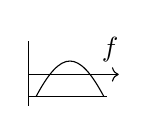
\begin{tikzpicture}
\draw (0,-0.12)--(0,0.7);
\draw (0,0)--(1,0);
\draw[->] (0,0.28)--(1.15,0.28);
\draw (0.1,0)..controls (0.42,0.6) and (0.64,0.6)..(0.96,0);
\node[above] at (1.04,0.32) {$f$};
\end{tikzpicture}
\end{adjustbox}
При почти всех $f$ трансверс. к $\Sigma^i$
Тогда применимы наивное опр. Тома и его прибл. к $\Sigma^i$;
т.е. $f\in\Sigma^I$ по Тому $\Longleftrightarrow$
росток $f$ в $\forall$ точке $\in\Sigma^I$ по Бордмэну.
Почти все трансверс. по общей теореме.
\underline{$R^n\longrightarrow R^n$}.
Когда впервые появл. особ. (точной коразм. $n$)
(Нужно точно описывать)
\begin{gather*}
\begin{array}{c|ccccccccc}
n&1&2&3&4&5&6&7&8&\text{9 (обведено)}\\
I&1&11&1_3&1_4&1_5&1_6&1_7&1_8&1_9\\
 & & & &2& & &2,1& &3
\end{array}
\end{gather*}
[Строки $n$ и $I$ разделены горизонтальной чертой.]
$x^2\quad\Sigma^{11}$ (сборка)
(Для общего отобр. точные. Это фактич. все,
дальше они не изв.)
[Ниже слева отдельный столбец, $10$ подчёркнуто:]
\begin{gather*}
10\\
1_{10}\\
2,2\\
2,1,1
\end{gather*}
[Справа:] В $R^4$ [зачёркнуто] $\Sigma$ — не полный набор инв.
\Unclear{GELFAND-P000181}{cancelled-invariants}{Между $R^4$ и $\Sigma$ зачёркнут маленький символ; исходная запись не установлена.}
В разм. $16$ особ. $4$ штуки.
\underline{$n=9$}:
\begin{gather*}
\text{на }M^8\text{ — одном. складки}\\
M^7\text{ — двум. сборки}\\
M^5\text{ — особ. типа }2.
\end{gather*}
Табл. легко сост. с помощью комбинат. ф-лы.
$1_9$ — ранг падает на $1$ на $M^8$, затем ещё на $1$ на $M^7$.

\SourcePage{GELFAND-P000182}{unlabelled}
\underline{Теорема} (Moren)
\Unclear{GELFAND-P000182}{theorem-name}{Имя в скобках выглядит «Moren» / «Morin» / «Морен»; соединённая третья буква и гласная не установлены уверенно.}
(обобщ. Уитни).
\begin{gather*}
j_0^{k+1}f\in\Sigma^{1_n0}\quad\Longleftrightarrow
\end{gather*}
\Unclear{GELFAND-P000182}{repeated-one-index}{Малый нижний знак при $1$ в верхнем индексе $\Sigma$ имеет густые соединённые штрихи: $n$ / $k$; заключительный $0$ виден отдельно.}
[Справа: «(напр. $110$) $0$ — трансверсальности.»]
$\exists$ координаты, в к-рых
\begin{gather*}
x_1=y_1\\
\ldots\\
x_{n-1}=y_{n-1}\\
y_n=x_1x_n+x_2x_n^2+\ldots+x_{n-1}x_n^{n-1}+x_n^{n+1}
\end{gather*}
(там сразу куб)
(Для классов $1_n$ особ. опр. с точн. до диффеом.)
Для типа $20$ класс не есть полный инвар.
(с точн. до диффеом.)
$\Sigma^{20}$ коразм. $4$
$f:R^4\longrightarrow R^4$
Мн-зие [зачёркнуто «особ.»-подобное] раздел. на $7$ кусков разной природы.
\Unclear{GELFAND-P000182}{cancelled-manifold}{После «Мн-зие» зачёркнуто сокращение, похожее на «особ.»; соединённые буквы под чертами не дают уверенного полного чтения.}
\underline{Квадратичный дифференциал отображения.}
$f:M^m\longrightarrow N^n$
(В $J^k$ две группы диффеоморфизмов $M^m$ и $N^n$ —
— \underline{возникают орбиты}. (в особых точках, какие орбиты))
\begin{gather*}
f_x:TM_x\longrightarrow TN_{f(x)}
\end{gather*}
Есть $Ker\,f_x\subset TM_x$, $Coker\,f_x=TN_{f(x)}/Im\,f_x$.
\begin{gather*}
f_{xx}:Ker\,f_x\longrightarrow Coker\,f_x
\end{gather*}
(квадратичное отображение, т.е. $\psi:A\longrightarrow B$
\begin{gather*}
A\overset{\Delta}{\longrightarrow}A\times A
\overset{\overline\psi}{\longrightarrow}B\\
\Delta\circ\overline\psi=\psi)
\end{gather*}
\underline{Опред. с пом. системы координат.}
\begin{adjustbox}{max width=\linewidth}
\begin{tikzpicture}
\draw[->] (-0.7,0)--(1,0);
\draw[->] (0,-0.6)--(0,0.8);
\node[below left] at (0,0) {$0$};
\node[below] at (1.1,-0.1) {$M$};
\draw[->] (2.3,0)--(4,0);
\draw[->] (3,-0.6)--(3,0.8);
\node[below left] at (3,0) {$0$};
\node[below] at (4.1,-0.1) {$N$};
\end{tikzpicture}
\end{adjustbox}
$X:TM_x\longrightarrow M$ (естеств. сист. коорд.)
$y:TN_y\longrightarrow N$ $(\xi\longrightarrow\xi t)$

\SourcePage{GELFAND-P000183}{43}
$\xi\in Ker\,f_x$
$X\xi$ — точка мн-зия
\begin{gather*}
\lim_{t\to0}\frac{\big(y^{-1}fX\xi t/Im\,f_x\big)}{t^2}
\end{gather*}
Легко док., что это не зав. от выб. сист. коорд.
(Кубич. дифф. так опр. нельзя)
Посмотреть!
Билин. отобр. $f_{xx}\Longleftrightarrow$ пучок квадр. форм.
Пусть $\alpha\in Co\,Coker\,f_0=C'$
[Под $Co\,Coker\,f_0$ скобкой вписано $(Coker\,f_0)'$.]
$\alpha f_{00}$ — квадр. форма на \underline{ядре}. (уже чистая кв. форма)
Плоск. в пр-ве квадр. форм.
Она не зав. от [зачёркнуто] выб. координат.
\Unclear{GELFAND-P000183}{cancelled-coordinates}{Перед «выб. координат» густо зачёркнута короткая запись; буквальные штрихи не установлены.}
\begin{gather*}
C'\longrightarrow\text{Кв}_{Ker\,f_0}
\end{gather*}
\underline{Пример.} $\Sigma^{20}:R^4\longrightarrow R^4$
\begin{gather*}
2=dim\,Ker\,f_0,
\end{gather*}
Отсюда $dim\,Coker\,f_0=2$
формы — $3$-хмерн. пр-во
(от $2$-х пер.)
\begin{gather*}
ax_1^2+2bx_1x_2+cx_2^2.
\end{gather*}
Есть классифик. по рангу
\begin{adjustbox}{max width=\linewidth}
\begin{tikzpicture}
\draw[->] (0,0)--(0,0.8) node[above]{$c$};
\draw[->] (0,0)--(0.9,0) node[below]{$b$};
\draw[->] (0,0)--(-0.5,-0.6) node[below]{$a$};
\end{tikzpicture}
\end{adjustbox}
$\text{Ранг}<2\ \Rightarrow$ конус $b^2=ac$ (инвар. опред.)
Ещё есть там плоскость (отобр. плоск. в пр-во квадр. форм).
Быв. разные располож. её
(пересек., касается, [зачёркнуто], с разных сторон $\pm$)
\Unclear{GELFAND-P000183}{cancelled-plane-position}{После «касается» зачёркнута запись с овальной петлёй / скобкой и нижними штрихами; буквальное чтение не установлено.}
Эти расположения, если они различны, то будут
(всего $7$ разн.) различные классы отобр.
с учётом вырожд.) И на самом деле $7$ орбит.

\SourcePage{GELFAND-P000184}{unlabelled}
\underline{Отобр. пишутся.}
\begin{gather*}
y_1=x_1x_2\\
y_2=x_1^2\pm x_2^2+\underbrace{x_1x_3+x_2x_4}_{\text{доб. для трансверсальности.}}\\
y_3=x_3\\
y_4=x_4
\end{gather*}
[Ниже две короткие горизонтальные черты.]
В $R^5$ быв. кривая $\Sigma^{20}$, где особ. различны вдоль кривой.
В компл. случае $\Sigma^{20}$ $\pm$ не отлич., но параб. случай остаётся.
\Unclear{GELFAND-P000184}{complex-case}{Сокращение после «но» выглядит «параб.» / «переоб.»; средние соединённые штрихи не дают уверенного полного чтения.}
$\Sigma^{20}$ — все особ. устойчивы, есть дифф. классиф.
$\Sigma^{30}$ — это \underline{уже не так.}
\underline{Теор. Тома.}
\begin{gather*}
\Sigma^{30}:R^9\longrightarrow R^9\\
dim\,Ker\,f_0=3\\
dim\,Coker\,f_0=3
\end{gather*}
[Справа:] пр-во особ. не дискретно (есть модули)
(Всё пока квадратичное)
\underline{Лемма.} При $n\geq3$ разм. орбиты
\begin{gather*}
GL(n,R)\times GL(n,R)
\end{gather*}
в $H(n,n)$ — квадр. формы $n$ перем.
(зам. перем.)
[От «зам. перем.» проведена ломаная скобка к межстрочной вставке:]
[зачёркнуто] в пр-ве и образе.
\Unclear{GELFAND-P000184}{lemma-interlinear}{Перед межстрочным «в пр-ве и образе» зачёркнут короткий знак с двумя соединёнными петлями; первоначальная запись не установлена.}
\begin{gather*}
codim\,\text{орбит}>0
\end{gather*}
(нет орбит полной разм.)
группа $2n^2$, формы $\dfrac{n^2(n+1)}{2}$, и всегда
есть одном. стац. подгруппа $\geq1$
(умн. на число там и там)
$\underline{n=3}$ и больше.
Отсюда и вытек., что сущ. модули.
\SourceFigure{GELFAND-P000184}{dimension-graph}{Внизу график с вертикальной осью $n$ и горизонтальной $m$, двумя восходящими прямыми из окрестности начала и рядом прямоугольников вдоль нижней из них. Видны подписи $n>2m$, «Уитни», «теор. Морса», у верхней области «влож.»-подобное, справа у прямоугольника «им. диал.»-подобное. Точные малые подписи, штрихи и границы прямоугольников требуют сопоставления с оригиналом.}
В клетке $9,9$ и $6,9$
выяснено, где есть модули
($J.$ Mather — анонсир.)
Он же — классифик. устойч. особ.

\SourcePage{GELFAND-P000185}{44}
\underline{Единств. инвар. устойч. особ. — локальное кольцо.}
\underline{Локальное кольцо} (инв., но все предид.) и \underline{подгот. теорема}
\begin{gather*}
f:M^m\longrightarrow N^n,\qquad f(0)=0.\\
O_* = E_x/(f_*\mathfrak M_1 E_y)E
\end{gather*}
\Unclear{GELFAND-P000185}{quotient-notation}{У $O$ нижний маленький знак густо переписан: $*$ / $x$ / $f$; в знаменателе после $\mathfrak M$ малый вертикальный штрих похож на $1$ / соединение. После скобки видно отдельное $E$.}
$E_x$ — кольцо ростков беск. дифф. ф-й на $M$ в $0$.
$E_y$ — аналог. от $y$
$\mathfrak M E_y$ — max идеал.
$f_*$ опр. естеств.
\underline{Смысл}: кольцо ф-й на слипшемся прообразе.
\underline{Пример.} $f(x)=x^2$,
\begin{gather*}
\mathfrak M E_y=yE_y=a_1y+\ldots\\
f_*\mathfrak M E_y=a_1x^2+a_2x^4+\ldots
\end{gather*}
\underline{Умн. на $E$}: всё больше $2$-й доб.
$a_1x^2+\ldots$
\underline{Факторизуем}: $a+bx$
\begin{adjustbox}{max width=\linewidth}
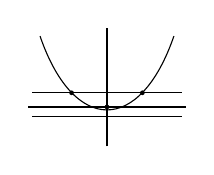
\begin{tikzpicture}
\draw (-1,0)--(1,0);
\draw (0,-0.5)--(0,1);
\draw (-0.85,0.9)..controls (-0.42,-0.35) and (0.42,-0.35)..(0.85,0.9);
\draw (-0.95,0.18)--(0.95,0.18);
\draw (-0.95,-0.12)--(0.95,-0.12);
\fill (-0.45,0.18) circle (0.03);
\fill (0.45,0.18) circle (0.03);
\fill (0,0) circle (0.03);
\end{tikzpicture}
\end{adjustbox}
кольцо ф-й на слипшихся $2$-х точках
(инфинит. пара точек)
\underline{Подвигаемся}: так и будет и пусть $y\longrightarrow0$.
[Обведено слева и снизу:]
$dim\,Q$ — кратность точки $0$ (в общ. случае)
\begin{gather*}
f:C^n\longrightarrow C^m
\end{gather*}
в аналит. случае
[Справа:] По-видимому, так.
\underline{Теорема} (Mather)
Устойч. особ. эквивал. $\Longleftrightarrow$ их лок. кольца совпадают.
\underline{Ещё одна теорема.} (Mather)
особ. устойчива $\Longleftrightarrow$ она инфинитезим. устойчива.
\underline{Последнее означает}:
В точке: $\underline{y=f(x)}$
\begin{adjustbox}{max width=\linewidth}
\begin{tikzcd}
x\arrow[r,"f"]\arrow[d,"h"']&y\arrow[d,"k"]\\
x\arrow[r,"g"]&y
\end{tikzcd}
\end{adjustbox}
$h$ и $k$ должны сущ. в беск. малом.
\SourceFigure{GELFAND-P000185}{vertical-field-graph}{Слева внизу оси $M$ и $N$, над $M$ волнистый график с максимумом и минимумом и рядом вертикальных отрезков, некоторые с наконечниками вверх. У крайнего левого отрезка густой наклонный штрих; точные направления всех стрелок и места их примыкания к кривой не установлены.}
график $f$
Сеч. рассл., пар. $N$.
Это также вект. поле
(вертик. вект. поле).

\SourcePage{GELFAND-P000186}{unlabelled}
Каждое вертик. поле $\varphi$ должно предст. в виде суммы.
\begin{gather*}
\varphi=f_*\xi+f^*\eta
\end{gather*}
(перенос)
[Справа над $f_*$ вертикальная стрелка вверх, над $f^*$ горизонтальная стрелка вправо.]
[Зачёркнуто] Можно пров., что ранее выпис. отобр. устойчивы.
\Unclear{GELFAND-P000186}{cancelled-check-word}{Перед «Можно пров.» зачёркнут короткий знак / сокращение с высокой верхней петлёй; исходная запись не установлена.}
\underline{Подгот. теор. Вейерштрасса}
(параметрическая редукция)
Если $Q$ конечномерно $(dim\,Q=r)$ и имеет образующие
\begin{gather*}
e_1(x),\ldots,e_r(x)
\end{gather*}
(ф-и, к-рые стан. образ. после факториз.)
то всякий росток $\varphi(x)\in E_x$ имеет [зачёркнуто] разложение:
\Unclear{GELFAND-P000186}{cancelled-expansion-word}{Под вставленным «имеет», перед «разложение», зачёркнуто связанное слово с начальной петлёй и несколькими нижними зубцами; чтение не установлено.}
\begin{gather*}
\varphi(x)=\psi_1(y)e_1(x)+\ldots+\psi_r(y)e_r(x)
\end{gather*}
$dim\,Q$ — прав. опр. кратности.
\underline{Теорема} (Mather)
\begin{gather*}
\Sigma^{20}\quad\text{разб. на части.}\\
1^\circ.\ \text{Пять серий колец }Q\\
2^\circ.\ \text{Остаток }codim=\infty
\end{gather*}
[Справа:] $f:M^m\longrightarrow N^n$
(надо опр. отобр. одной из серий)
Особенности пяти серий устойчивы:
\begin{gather*}
\begin{array}{lll}
n\geq m1.&I_{a,b}&R[x,y]/\{x,y,x^a+y^b\}\qquad b\geq a\geq2\\
n\geq m2.&II_{a,b}&/\{xy,x^a-y^b\}\qquad b\geq a\geq2\quad\text{чётные}\\
n>m3.&III_{a,b}&/\{x^a,y^b,xy\}\\
n>m4.&IV_a&/\{x^a,xy^{a-1},x^2+y^2\}\qquad a\geq3\\
&V_a&/\{x^a,x^2+y^2\}\qquad a\geq3
\end{array}
\end{gather*}
\Unclear{GELFAND-P000186}{series-one-ideal}{В знаменателе первой строки между $x$ и $y$ виден отдельный низкий штрих, похожий на запятую; запись сохранена как $\{x,y,x^a+y^b\}$, кандидат $\{xy,x^a+y^b\}$ остаётся отдельно.}
\Unclear{GELFAND-P000186}{series-dimension-left}{Слева четыре строки выглядят $n\geq m1.$, $n\geq m2.$, $n>m3.$, $n>m4.$; между $m$ и цифрами отдельный плюс / минус не различён. Цифры могут быть нумерацией строк или частью сокращённого условия.}
Посчитаны коразмерности.
(для всех серий)
Симв. $\Sigma^{20}$ рассл. на подмн-зия
(Это самый сильный рез. о классифик. особенностей)
\underline{След. раз $13/II$} — $1967$ г.

\SourcePage{GELFAND-P000187}{unlabelled}
\underline{Сем. Гельфанда.}
\underline{План.}
\begin{gather*}
\begin{array}{lll}
1.&\text{Кириллов Harish-Chandra}&\approx10\ \text{лекций.}\\
2.&\text{Аносов Маслов и квазиклассика}&2\ \text{лекции.}\\
3.&\text{Каждан A. Weil.}&6\text{–}7\ \text{лекций.}\\
4.&\text{Дынкин Индекс.}&3\ \text{лекции.}\\
5.&\text{Аносов Ур-я Пфаффа (1-го порядка)}&1\ \text{лекция.}\\
6.&\text{KG-функтор (Бернштейн)}&2\ \text{лекции.}
\end{array}
\end{gather*}
В след. раз \underline{Кириллов} и \underline{Аносов}.
\underline{Кириллов Лекция 1.}
Серия раб. H.-Ch., прив. к опис. всех предст. вещ. полупр. групп Ли.
[Над «предст.» обведена вставка: «непр. унит.»]
Сегодня схема док-ва одной теоремы (о характерах).
$G$ — вещ. полупр. группа Ли. (редуктивная — для инд.)
На ней рассм. дифф. опер. перест. и с левыми и с пр. сдвигами.
Это кольцо мног. от образ.
\begin{gather*}
D_1,\ldots,D_\ell\quad\text{— ранг группы.}\\
G=SL(n),\qquad\ell=n-1,
\end{gather*}
по $1$ му степ. всех степ., начиная со второй.
\underline{Гельфанд}: $E_{ik}$
\begin{gather*}
x=(\ldots),\qquad f(x(1+te_{ik}))=f(x)+tE_{ik}f+\ldots
\end{gather*}
В полной группе $\sum E_{ii}$ (он трив. в $SL$)
\begin{gather*}
\sum E_{ik}E_{ki}\\
\sum E_{ij}E_{jk}E_{ki}\\
\ldots
\end{gather*}
Ост. выраж. через первые $n$.
(см. Гельфанд, \underline{1947})
\underline{К.} Рассм. обобщ. ф-и на группе, явл. реш. всех этих ур-й.
$R$ — кольцо всех мног. от $D_1,\ldots,D_\ell$.
$J$ — [зачёркнуто] идеал, такой что $dim\,(R/J)<\infty$.
\Unclear{GELFAND-P000187}{cancelled-ideal}{Перед «идеал» зачёркнуто слово, похожее на «все» / «всё»; горизонтальные черты пересекают средние буквы.}

\SourcePage{GELFAND-P000188}{51}
Рассм. обобщ. ф-и $T$, такие что
\begin{gather*}
T^x=T\quad\text{для }x\in G
\end{gather*}
($x$ — внутр. автом.) — пост. на классах сопр. элем.
\begin{gather*}
\langle T^x,f\rangle=\langle T,f^{x^{-1}}\rangle,\qquad
f^{x^{-1}}(y)=f(x^{-1}yx)
\end{gather*}
\underline{Г.}: $D_1,\ldots,D_\ell$ — операторы Лапласа на группе.
Пусть $D_iT=\lambda_iT$, тогда $T$ — соб. ф-я (обобщ.)
Среди них ищ. «сферич. симм.» (зональные)
\begin{gather*}
T(y)=T(x^{-1}yx)
\end{gather*}
Тогда она настоящая и притом \underline{суммируемая} (локально)
[На правом поле подчёркнута запись:]
\Unclear{GELFAND-P000188}{margin-name}{Имя на поле похоже на «Schwartz» / «Schwarz»; средние соединённые буквы стянуты и пересечены длинной нижней чертой.}
Можно рассм. присоед. соб. ф-и:
\begin{gather*}
(D-\lambda)^2T=0
\end{gather*}
(не $R$, а $JT=0$).
\begin{gather*}
r(D_1,\ldots,D_\ell)T=0,\qquad r\in J.
\end{gather*}
Для max идеала это просто соб. ф-и $(\lambda_i)$
\underline{Она не обязательно непрерывна!}
\underline{К.}
\begin{gather*}
1)\quad T^x=T\quad\text{для }x\in G\\
2)\quad DT=0\quad\text{для }D\in J
\end{gather*}
Тогда она лок. суммируема.
Коммут. группа $\Rightarrow$ все дифф. опер., далее аналит.,
т.к. есть эллипт. ур-е.
\underline{Общ. идея}: в окр., ф-и, зав. фактич. от $\ell$ парам.,
удовл. $\ell$ ур-ям, устр. эллипт. ур-е, вне особых точек.
Характеры обращ. в $1$ в $\infty$ — могут иметь разрывы.
\underline{Как это док.?}
Мн-во классов сопр. элем. устр. так: откр. подмн.,
явл. подмн-зиями
$GL(n)$ — различные соб. значения.
Диагон. коразм. $2$ или $3$ в свою очередь
имеет подмн. и т.д. ($2$ соб. знач. совп. и т.д.) —
— стратификация.

\SourcePage{GELFAND-P000189}{unlabelled}
В рег. точке $y\in G$ это аналит. ф-я.
В окр. $y$ устр. новая сист. коорд.
\begin{adjustbox}{max width=\linewidth}
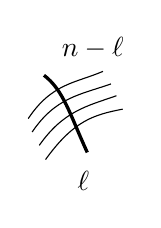
\begin{tikzpicture}
\draw (0,0)..controls (0.3,0.45) and (0.6,0.45)..(0.95,0.6);
\draw (0.05,-0.17)..controls (0.35,0.27) and (0.65,0.3)..(1.05,0.44);
\draw (0.14,-0.34)..controls (0.45,0.1) and (0.75,0.16)..(1.12,0.29);
\draw (0.22,-0.52)..controls (0.58,-0.02) and (0.84,0.05)..(1.2,0.12);
\draw[very thick] (0.2,0.55)..controls (0.45,0.36) and (0.53,0.05)..(0.75,-0.43);
\node[above] at (0.82,0.64) {$n-\ell$};
\node[below] at (0.7,-0.55) {$\ell$};
\end{tikzpicture}
\end{adjustbox}
[Справа от семейства линий: «классы сопр. элем.»;
от $\ell$ отведён указатель: «трансверс. сечение.»]
На $U\times V$ есть обобщ. ф-я, не завис. от [зачёркнуто] одной коорд.,
\Unclear{GELFAND-P000189}{independent-coordinate}{Между «от» и «одной коорд.» густо перечёркнут малый знак, похожий на $V$ / $\forall$ / иной знак; «одной» оставлено как видно.}
свод. к обобщ. ф-и на сечении. (см. L. Schwarz)
\begin{gather*}
D_1,\ldots,D_\ell
\end{gather*}
порожд. почти все дифф. опер. на сечении
(уже конечн. коразм. в кольце всех дифф. опер.)
\begin{gather*}
\Delta=D_1^2+D_2^2+\ldots+D_\ell^2
\end{gather*}
уже эллиптич. на сечении.
при этом
\begin{gather*}
\Delta^n+c_1\Delta^{n-1}+\ldots+c_n\in J
\end{gather*}
Итак, $\Delta T=0$, $\Delta$ — эллипт.
Произв. случай свод. к этому индукцией по разм. группы.
\underline{$3$ разных случая.}
\begin{gather*}
x\quad\text{— }1)\ \text{полупр.}\\
2)\ \text{нильпот.}\\
3)\ \text{единичный.}
\end{gather*}
$1)$ — свод. к централизатору $y$ — редукт. группа,
если $y$ не из центра. (тогда вся группа)
[Над «редукт. группа» обведено: «меньшей разм.»]
$2)$ нильп. — особый приём
$3)$ $x=e$ — $\ln$, $\exp$ свод. к исслед. алгебры Ли —
— $2$ отд. работы.
Идея для полупр. элем. — переход к пол. коорд.
(рад. часть опер. Лапласа)
$\underline{a\text{ — полупр. элемент}}$
[Справа за вертикальной чертой:] $G$ действ. на [зачёркнуто] $g$ —
— алг. Ли
\Unclear{GELFAND-P000189}{cancelled-action}{После «на» перед $g$ зачёркнут символ с петлёй и длинным нижним штрихом, похожий на $g$ / иной знак; первоначальная запись не установлена.}
если $\underline{Ad_a}$ $(z\longrightarrow aza^{-1})$
прив. к диаг. виду, т.е. без жорд. клеток
(Для $SL(n)$ — сама матр. не им. жорд. клеток)
$z$ — централизатор [зачёркнуто] $a$ в алгебре.
\Unclear{GELFAND-P000189}{cancelled-centralizer}{Перед $a$ после «централизатор» густо переписан / зачёркнут малый символ с несколькими петлями; исходное чтение не установлено.}
(для [зачёркнуто] — картановская подалгебра)
[Над зачёркнутым фрагментом обведена вставка: «регул. элем.»]
\Unclear{GELFAND-P000189}{cancelled-cartan}{В скобках после «для» под вставкой «регул. элем.» зачёркнута запись, похожая на $a$ / $x_0$ / иной символ; несколько исходных штрихов соединены с отменяющими чертами.}
\SourcePage{GELFAND-P000190}{52}
% Original: 2024 x 2415 px; reading order: single visible leaf, top to bottom.
Провести сечение (пока ещё избыточное)

Теор. Березина для регул. элементов --- огранич. опер.
на карт. подалгебру.

$\Xi$ --- группа Ли, соотв. $\mathfrak z$.

Устр. отобр.
\begin{align*}
\varphi\colon G\times\Xi&\longrightarrow G\\
(x,y)&\longmapsto (ay)^x=xayx^{-1}
\end{align*}

Еще обознач.:
\begin{gather*}
V_a(y)=\det\bigl(\operatorname{Ad}(ay)^{-1}-1\bigr)_{\mathfrak g/\mathfrak z}\\
\Xi'=\{y\in\Xi:V_a(y)\ne0\}\quad\text{--- «рег. точки» }\Xi
\end{gather*}
($V_a\ne0$, т.к. уже нет соб. знач. $1$, оно на $\mathfrak z$)

\underline{Теор. 1} \quad (лемма 14)
\begin{equation*}
\operatorname{rang}d\varphi=n=\dim G\qquad\text{на }G\times\Xi'
\end{equation*}
(локально это $\max$ ранга --- типа проекции)

\underline{Док-во.} $X,Z$ --- пара кас. вект.
\begin{equation*}
d\varphi(X,Z)=Z+\bigl(\operatorname{Ad}(ay)^{-1}-1\bigr)X,
\end{equation*}
откуда всё следует.

На факторе невырожд.

$Z$ обесп. полный ранг на всём пр-ве.

\underline{Результат из др. работы.}
\begin{equation*}
d\mu\quad M^m\overset{\pi}{\longrightarrow}N^n\quad d\nu
\quad\text{--- меры},\qquad m\ge n
\end{equation*}
$\operatorname{rg}d\pi=n$.

Можно с $M$ на $N$ переносить обобщ. ф-и
(\Unclear{GELFAND-P000190}{lower-local-mark}{\underline{\underline{Г}}?}: локально)
\begin{equation*}
\alpha\in C_0^\infty(M)\quad\longrightarrow\quad f_\alpha\in C_0^\infty(N),
\end{equation*}
так что $\forall F$ на $N$ будет
\begin{equation*}
\int_M\alpha\cdot F\circ\pi\,d\mu=\int_N Ff_\alpha\,d\nu
\end{equation*}
(Для [зачёркнуто: \Unclear{GELFAND-P000190}{bottom-cancelled-product}{$M\times$?}]
$N\times\ldots$ это интегр. по лишним перем.)

это делается линейно, разб. единицы, лок. это
прямое произв.

\SourcePage{GELFAND-P000191}{unlabelled}
% Original: 2024 x 2415 px; no confidently visible leaf label.
\underline{Перспектива:} примен. к $\varphi$.

\underline{Полезное обозначение.} (для нечитабельности)

На $M\times N$ есть функция (гладкая)

$D_1,D_2$ --- дифф. опер. на $M,N$.
\begin{equation*}
f(x;D_1:y;D_2)=(D_{1x}\times D_{2y}f)(x,y)
\end{equation*}
(прим. $D_1$ по $x$ и $D_2$ по $y$)

Единичный опер. опускается.
\begin{equation*}
f(x:y;D_2)\quad\text{---}
\end{equation*}
--- объяснено лишь в одной работе.

\underline{Ещё одно обозначение.}
\begin{equation*}
G,\quad f(x)\text{ на }G,\qquad f(x:y)=f(xyx^{-1})
\end{equation*}
В след. раз. обобщ. теор. Березина.

\underline{Для ед. опер.} $D_1$ и $D_2$:
\begin{equation*}
f(x:y)
\end{equation*}
и к ней всё применяется.

\bigskip
\underline{Дынин.}

$X$ --- гладкое комп. мн-зие

$E_1,E_2$ --- рассл. на $X$
\begin{equation*}
A\colon\Gamma(E_1)\longrightarrow\Gamma(E_2)\quad\text{--- лин. дифф. опер.}
\end{equation*}

\underline{Псевдодифф. опер.}

$\{U_i\}$ \qquad $\varphi_i$ --- впис. разб. $1$
\begin{equation*}
\psi_i\varphi_i=\varphi_i
\end{equation*}
1) $\psi_i A(\varphi_i\,\cdot)$ --- обычн. псевдодифф. опер. в пр-ве
вектор-ф-й

2) $\varphi\psi=0\ \Rightarrow\ \psi A(\varphi\,\cdot)$ сглаживающий опер.

\SourcePage{GELFAND-P000192}{53}
% Original: 2024 x 2415 px; handwriting occupies the top approximately 960 px.
\underline{Пример:}
\begin{equation*}
d\colon\Gamma(\Lambda T(x))\longrightarrow\Gamma(\Lambda T(X))
\end{equation*}
$\overset{!}{\text{всё}}$ формы (неоднор.)
\begin{equation*}
\Lambda T(X)=\bigoplus_k\Lambda^kT(x)
\end{equation*}
\Unclear{GELFAND-P000192}{upper-form-notation}{[регистр $x/X$ в обозначениях $T(x)$ и $T(X)$ не вполне различим]}

$\delta\colon$ \quad --- сопр. опер. (по рим. метрике)
\begin{equation*}
\delta=d^*.
\end{equation*}
\Unclear{GELFAND-P000192}{upper-operator-name}{$d+\delta$ --- опер. Коши-Римана}

\begin{equation*}
\Delta=(d+\delta)^2\quad\text{--- опер. Лапласа.}
\end{equation*}
\begin{equation*}
\Delta\colon\Gamma(\Lambda^kT(X))\longrightarrow\Gamma(\Lambda^kT(X)).
\end{equation*}
Теорема Ходжа:
\begin{equation*}
\ker\Delta\big|_{\Gamma(\Lambda^kT(X))}=H^k(X,C)
\end{equation*}
(очень простой факт, см. Морен, связь с ур. теплопроводности)

\underline{След. раз.}
\begin{gather*}
6\text{--}7\quad\text{--- Кириллов}\\
7\text{--}8\quad\text{--- Аносов.}
\end{gather*}

\SourcePage{GELFAND-P000193}{unlabelled}
\begin{center}
\underline{Сем. Гельфанда.} $20/\mathrm{II}$.\\
\underline{Кириллов.}\qquad \underline{Лекция 2.}
\end{center}
Случай, когда слой полож. размерности. $(xyx^{-1})$ —
— $y$ не из центра.

Пусть $a$ — полупростой элемент.
Пров. сеч., пересек. по 1-му элем. с люб. классом сопр. элем.
\begin{gather*}
\mathfrak g\text{ — алг. Ли},\qquad
\mathfrak z=\{X:\operatorname{ad}_a X=X\},\qquad \Xi\subset G.
\end{gather*}
[Под $\Xi$: подгр., соотв. $\mathfrak z$.]

Сечение — связн. компон. централизатора $a$.
Всё сведётся к группе $\Xi$.
Построим новую обобщ. ф-ю и дифф. опер.
Как задавать дифф. опер. на группе Ли?
Рассм. левоинвар. дифф. опер. ($\exists$ левоинв. $\forall$ точке,
совп. с нашим с точн. до мл. членов)

$D_y$ — левоинв. опер., к-рый в $y$ совп. с $D$.

\Unclear{GELFAND-P000193}{middle-operator-algebra}{$D_y\in\mathfrak g$} — опис. весь оператор (сразу на всей группе)

Будем огранич. дифф. оператор на подмн-ве

\begin{center}
\begin{adjustbox}{max width=\linewidth}
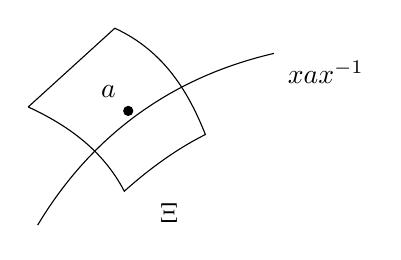
\begin{tikzpicture}[x=1cm,y=1cm]
\draw (0,1.5) -- (1.1,2.5) .. controls (1.75,2.2) and (2.05,1.65) .. (2.25,1.15)
.. controls (1.85,0.95) and (1.5,0.68) .. (1.22,0.43)
.. controls (0.95,0.95) and (0.5,1.27) .. (0,1.5);
\draw (0.12,0) .. controls (0.6,0.8) and (1.48,1.8) .. (3.12,2.18);
\fill (1.27,1.45) circle (0.065);
\node at (1.02,1.7) {$a$};
\node at (3.78,1.94) {$xax^{-1}$};
\node at (1.79,0.15) {$\Xi$};
\end{tikzpicture}
\end{adjustbox}
\end{center}
Дифф. вдоль слоёв будем считать нулями.
Слои, близкие к $a$, могут иметь большую размерность.

\begin{gather*}
f(x;D_1:y;D_2)=\underline{f(x:y;\Gamma_y(D_1\otimes D_2))}
\end{gather*}
($D_1$ по $x$, $D_2$ по $y$)

[Под формулой, в обводке: \Unclear{GELFAND-P000193}{lower-definition-note}{опред. $\Gamma_y$;?}]

Явный вид замены опер. по обоим пер. на опер. по $y$.
\begin{gather*}
\frac{\partial^2 f}{\partial x\partial y}
=f(x;\Unclear{GELFAND-P000193}{bottom-first-operator}{d\text{ или }\partial}:y;d)
\end{gather*}
$\Gamma_y$ — билин. зав. от $D_1,D_2$ или — лин. от $D_1\otimes D_2$.

\SourcePage{GELFAND-P000194}{57}
\underline{Явное выраж.} $\Gamma_y$. ($g_1,g_2$ — элем. обёрт. алгебры.
\begin{gather*}
f(x;g_1:y;g_2)=f(x:y;\Gamma_y(g_1\otimes g_2)).\\
\Gamma_y(g_1\otimes g_2)=\sigma_y(g_1)\cdot g_2,
\end{gather*}
где $\sigma_y(g_1)$ — представление обёрт. алгебры, т.е.
$\sigma_y(gh)=\sigma_y(g)\sigma_y(h)$.

Теперь $\sigma_y$ дост. выч. на образ. обёрт. алгебры.
\begin{gather*}
\sigma_y(X)=L_{X^{y^{-1}}}-R_X\qquad (X\text{ из алгебры Ли}).\\
\sigma_y(X):g\longrightarrow X^{y^{-1}}g-gX
\end{gather*}
\underline{\underline{Вывод.}}
[Зачёркнуто: \Unclear{GELFAND-P000194}{upper-cancelled-start}{(ст…}]
(старш. член) — на базисе:
\begin{gather*}
\Gamma_y(X_1\cdots X_r\otimes Y_1\cdots Y_s)
=X'_1\cdots X'_r\Unclear{GELFAND-P000194}{upper-y-superscript}{Y_1^{\ast}?}\cdots Y_s;\\
\underline{X'_i=(\operatorname{ad}y^{-1}-1)\cdot X_i}
\end{gather*}
[Зачёркнуто: \Unclear{GELFAND-P000194}{middle-cancelled-formula}{$f(x;g_1$?}]

\underline{Г.}
\begin{gather*}
X_1X_2\cdots X_rY_1\cdots\Unclear{GELFAND-P000194}{middle-last-y-index}{Y_r}\,f(xyx^{-1})
\end{gather*}
Надо перенести опер. на $y$, $Y_i$ остаётся, а
[зачёркнуто: \Unclear{GELFAND-P000194}{middle-cancelled-word}{если?}]
если $X$ коммут. с $y$, то ничего не изм.

(Легко всё [вставлено: это] проверить)
\begin{center}
— · —
\end{center}
\underline{К.}
\begin{center}
\begin{adjustbox}{max width=\linewidth}
\begin{tikzcd}[column sep=small,row sep=small]
\Gamma_y: & \mathfrak g\otimes\mathfrak g \arrow[r] & \mathfrak g && \text{(}\mathfrak g\text{ — обёрт. алгебра)} \\
& \cup\quad\cup \\
0 \arrow[r] & \underline{\underline{\mathfrak q}}\otimes\underline{\underline{\mathfrak z}}
\arrow[r,"\Gamma_y"] & \mathfrak g \arrow[r] & 0 & \text{изоморфизм!}
\end{tikzcd}
\end{adjustbox}
\end{center}
\Unclear{GELFAND-P000194}{lower-algebra-notation}{$\mathfrak g=\mathfrak z+\mathfrak q$},
[зачёркнуто: \Unclear{GELFAND-P000194}{lower-cancelled-word}{где?}]
$\mathfrak q$ — доп. подпр-во, инвар.
отн. $\operatorname{Ad}\mathfrak z:\ [\mathfrak z,\mathfrak q]\subset\mathfrak q$.

$\underline{\underline{\mathfrak z}},\ \underline{\underline{\mathfrak q}}$
уже порожд. ими в обёрт. алгебре.

Выберем $y$ регулярным (т.е.
$\Unclear{GELFAND-P000194}{bottom-regularity-symbol}{\nu_a(y)\text{ или }v_a(y)\text{ или }V_a(y)}\ne0$).
Тогда отобр.
$\Gamma_y$ по ф-ле невырождено и в ст. чл. однозначно,

\SourcePage{GELFAND-P000195}{unlabelled}
$D$ — опер. на группе,
\begin{gather*}
D\longrightarrow
\underbrace{\delta_{a,\,G\Unclear{GELFAND-P000195}{top-delta-separator}{\vert\text{ или }/}\Xi}(D)}_{\Delta}
\end{gather*}
— опер. на $a\Xi$ —
— подмн-зие.

Соотв. постр. так, что для ф-й, пост. на траект.
всё равно.

[Зачёркнута формула: \Unclear{GELFAND-P000195}{upper-cancelled-formula}{в начале $\varphi$?, в конце $(D)$?}.
\Incomplete{GELFAND-P000195}{upper-cancelled-formula}{Остальная часть зачёркнутой формулы неразборчива.}]
\begin{gather*}
\Delta_{ay}=\alpha(D_{ay})\\
D-\alpha(D)\in\Gamma_y(\mathfrak q^+\otimes\mathfrak z)
\end{gather*}
($\alpha(D)$ — своб. член $D$. $\mathfrak q^+$ — элем., не
имеющие своб. члена).

След. раз ещё перенос обобщ. ф-й.

\bigskip
[Над датой — короткий дугообразный штрих.]
\begin{center}
$27/\mathrm{II}$\qquad \underline{Сем. Гельфанда.}\\
\underline{Кириллов, Лекция 3.}\\
\underline{Перенос обобщённых функций.}
\end{center}
Рассм. вспомог. отображение:
\begin{gather*}
\varphi:G\times\Xi'\longrightarrow G\\
(x,y)\longrightarrow xayx^{-1}
\end{gather*}
($\Xi'$ — регул. элем. $\Xi$,
$\Unclear{GELFAND-P000195}{lower-regularity-symbol}{\nu_a(y)\text{ или }v_a(y)\text{ или }V_a(y)}\ne0$)
\begin{gather*}
\operatorname{rank}\varphi=\dim G.
\end{gather*}
Теперь переносятся с $G$ на $\Xi$ обобщ. ф-и.
Сначала они переносятся на $G\times\Xi'$.

$T$ — обобщ. ф-и на $G$.

Надо науч. переносить обычн. ф-и в прямую
сторону. Это, грубо говоря, интегрирование (локально).

\SourcePage{GELFAND-P000196}{58}
\begin{equation*}
M\longrightarrow N,\qquad C_c^{\infty}(M)\longrightarrow C_c^{\infty}(M)
\end{equation*}
\Unclear{GELFAND-P000196}{top-codomain}{[В правом пространстве функций написано $M$.]}

На $M$ и $N$ зад. объемы $dx$ и $dy$. (дифф. формы)
\begin{equation*}
\alpha(x)\longrightarrow f_{\alpha}(y)
\end{equation*}
Должно быть вып. условие: $\forall F(y)$
\begin{equation*}
\int_M\alpha(x)F(\varphi(x))\,dx
=\int_N F(y)f_{\alpha}(y)\,dy
\end{equation*}
\underline{Теорема}: такое отобр. сущ. и непр. в топ. этих пр-в.

\underline{Пример.}
\begin{equation*}
\begin{array}{ccccc}
M&=&N&\times&P\\
&&dy&&dz
\end{array}
\qquad (dx=dy\,dz).
\end{equation*}
Тогда отобр. — интегрирование по $z$.

\begin{center}
— · —
\end{center}

[Перед $G\times\Xi'$ зачёркнуто:
\Unclear{GELFAND-P000196}{middle-cancelled-prefix}{$M$ или $\forall M$}.]
\begin{equation*}
\begin{adjustbox}{max width=\linewidth}
\begin{tikzcd}[row sep=small,column sep=large]
G\times\Xi' \arrow[r,"\varphi"] & G \\
\underset{\text{обобщ. ф-и}}{\underline{T'}} & T\text{ — обобщ. ф-и на }G \arrow[l]
\end{tikzcd}
\end{adjustbox}
\end{equation*}
$T'$ по 1-му сомнож. инвар. отн. сдвигов
\begin{equation*}
\langle T',f(x,y)\rangle=\langle T',f(x'x,y)\rangle
\end{equation*}

\underline{Лемма.}

обобщ. ф-я, инвар. отн. сдвигов, есть $\int$ по мере Хаара
$(\mathrm{const})$

\begin{center}
— · —
\end{center}

$T'$ зависит только от 2-го аргумента (проинт. по 1-му).
\begin{equation*}
T'=1\otimes\sigma_T
\end{equation*}
Можно дать явную ф-лу, выраж. $\sigma_T$ через $T$ (К.)
\begin{equation*}
\langle\sigma_T,\beta\rangle
=\left\langle T,\int_G\gamma(z)\beta(a^{-1}z^{-1}xz)\,dz\right\rangle,
\end{equation*}
[Справа под формулой:] $\beta$ — ф-я на $\Xi$

где $\gamma(z)$ — любая ф-я, удовл. условию
\begin{equation*}
\int_G\gamma(z)\,dz=1
\end{equation*}
\SourceFigure{GELFAND-P000196}{bottom-diagonal-note}{[Наклонная пунктирная черта идёт от левого верхнего края формулы для $\langle\sigma_T,\beta\rangle$ через её область к помете внизу справа; точное назначение черты неясно.]}
[Внизу справа:] Она не имеет смысла.

\SourcePage{GELFAND-P000197}{unlabelled}
Итак, имеем:
\begin{equation*}
\begin{aligned}
D&\longrightarrow\Delta=\delta_{a,G/\Xi}(D)\\
T&\longrightarrow\sigma_T
\end{aligned}
\end{equation*}
\Unclear{GELFAND-P000197}{top-sigma-prime}{[После $\sigma$ в нижней строке тонкий штрих: $\sigma'_T$ или $\sigma_T$.]}
[Обе стрелки вместе подчёркнуты.]

$a\in U_G\subset G$\qquad
[Зачёркнуто: \Unclear{GELFAND-P000197}{top-cancelled-xi}{$\Xi$?}.]
$\Xi\supset U_{\Xi}\ni1$

\underline{Лемма.}
\begin{equation*}
\sigma_{DT}=\Delta\sigma_T
\end{equation*}
(Существ. использование $\Gamma_{ay}:\mathfrak g\times\mathfrak g\longrightarrow\mathfrak g$.)

\underline{Факты.}

1) Операторы $\Delta$ порождают идеал конечн. коразм. в центре гр. $\Xi$.

(На карт. подалгебре это опер., симм. отн. группы Вейля)
\begin{equation*}
\begin{adjustbox}{max width=\linewidth}
\begin{tikzcd}[row sep=small,column sep=large]
G & \Xi \\
\mathfrak g \arrow[r,"\alpha"] & \mathfrak z \\
Z(\mathfrak g) \arrow[r] & Z(\mathfrak z)
\end{tikzcd}
\end{adjustbox}
\end{equation*}
$Z(\mathfrak g)$ — центр обёрт. алгебры, образ $Z(\mathfrak g)$ лежит
в центре $Z(\mathfrak z)$ (можно пров.), а идеал, им
порожд., конечной коразмерности.
\begin{equation*}
\begin{adjustbox}{max width=\linewidth}
\begin{tikzcd}[row sep=small,column sep=large]
\cup & \cup \\
I \arrow[r] & J
\end{tikzcd}
\end{adjustbox}
\end{equation*}

Тогда получ. полная редукция к $\Xi$
\begin{equation*}
\sigma_T\text{ — лок. суммир.}\quad\Longrightarrow\quad
T\text{ тоже лок. суммир.}
\end{equation*}
$a$ в центре $\Longrightarrow$ свод. сдвигом
[зачёркнуто: \Incomplete{GELFAND-P000197}{bottom-cancelled-before-case}{Текст полностью перекрыт штрихами и не прочитан.}]
к случаю $a=e$,
там особая техника (3 работы
[зачёркнуто: \Incomplete{GELFAND-P000197}{bottom-cancelled-before-name}{Текст полностью перекрыт штрихами и не прочитан.}]
Хариш-Чандры)

\SourcePage{GELFAND-P000198}{59}
$6/\overline{\underline{\mathrm{III}}}$. \underline{Сем. Вишика.}

1. Продолжение докл. Аграновича.

2. Продолжение докл. Г. И. Эскина.

\begin{center}
\underline{Сем. Гельфанда.}
\end{center}

[На левом поле:] \underline{Кириллов}

$x^2+y^2-z^2=c$, $T$ инвар. отн.
[Зачёркнуто: \Unclear{GELFAND-P000198}{invariance-cancelled}{этой гр... / этой ф...}]
группы, сохр. эту ф-ю.

\begin{equation*}
P\left(\frac{\partial^2}{\partial x^2}
+\frac{\partial^2}{\partial y^2}
-\frac{\partial^2}{\partial z^2}\right)T=0,
\end{equation*}
будет ли $T$ лок. суммир.?

[Зачёркнуто: \Incomplete{GELFAND-P000198}{parenthesis-cancelled}{неразборчивое зачёркнутое слово}.]
($T$ --- замык. лок. ф-й, пост. на слоях)

\SourceFigure{GELFAND-P000198}{cone-sketch}{Слева нарисованы большой верхний овал, меньшая верхняя петля и нижний овал; две диагональные линии пересекаются, образуя двойной конус. По бокам проходят вогнутые кривые; внутри верхней и нижней частей есть дополнительные дуги. У нижних концов диагоналей --- утолщения, возможно наконечники стрелок. Уверенно читаемых подписей нет; принадлежность внутренних дуг и утолщений требует проверки.}

Вне конуса сист. эллиптична.

\underline{Арнольд.}

\underline{C. J. Earle, J. Eells.}

$X^2$ --- 2-мерн. комп. мн-зие (ориент.)

$\operatorname{Diff}_0(X)$ --- группа его диффеом., гомот. тождеств.

\underline{Вычислена её топология!}

\begin{equation*}
\operatorname{Diff}_0 X=
\left\{
\begin{array}{ll}
X=S^2\,: &
\underset{\substack{\text{конф.}\\\text{отобр.}}}{G}
\times
\underset{\text{стягив.}}{\underline{\operatorname{Diff}(S^2-a,b,c)}}
\quad (a,b,c\;\text{на месте})\\
X=T^2 &
T^2\times\underset{\text{стяг.}}{\operatorname{Diff}(T^2-a)}\\
\text{род}\geq 2 & D\sim 0\qquad\text{стягиваема}
\end{array}
\right.
\end{equation*}
[Знак после $X=S^2$: \Unclear{GELFAND-P000198}{sphere-case-separator}{двоеточие с дополнительным штрихом / знак из трёх точек}.]

Док-во осн. на раб. \Unclear{GELFAND-P000198}{ahlfors-name}{Альферса / Альфорса}
и Берса по квазиконф. отобр., на к-рые стяг. любое дифф.

$\operatorname{Diff}$ --- группа Ли в новом поним. гладк. структуры.

\SourcePage{GELFAND-P000199}{unlabelled}
\underline{Аносов.}

\underline{Постановка задачи.}
[Подчёркнуто штрихами.]

$Lu=f$, $u(x)\in H$, $H$ --- гильбертово.

В $H$ есть опер. $A$, $0$ --- не собств. знач., $A$ --- самосопр.

$L$ может зависеть и от $A$.

\begin{center}
\begin{adjustbox}{max width=\linewidth}
\begin{tikzpicture}
\node at (0,0) {$-\dfrac{h^2}{2}\dfrac{d^2}{dx^2}+U(x)$};
\node at (0,-1.4) {$\dfrac{p^2}{2}+U\left(\dfrac{h}{i}\dfrac{d}{dp}\right)$};
\draw[->,line width=1pt] (2.1,0) .. controls (3.1,-0.25) and (3.1,-1.05) .. (2.1,-1.4);
\node[anchor=west] at (3.0,-0.7) {преобр. Фурье с коэфф. $h$};
\end{tikzpicture}
\end{adjustbox}
\end{center}
[Стрелка в рукописи широкая, заштрихована.]

(псевдодифф. оператор) ---
$\overline{\mathcal{F}}_{p\to x}\,\sigma(x,p)\,\mathcal{F}_{x\to p}\,f(x)$

\begin{equation*}
e^{\pm i\frac{1}{h}(p,x)}=
\end{equation*}
($h$ для безразмерности).

По Маслову $\dfrac{1}{h}$ оператор; т. к. всё ф-и $h$

\begin{equation*}
=e^{\pm iA(p,x)}
\end{equation*}

$A$-преобразование Фурье:

\begin{equation*}
\phi^A_{x\to p}f(x)=\left(\int e^{iA(x,p)}f(x)\,dx\right).
\end{equation*}
[Перед интегралом вставлен обведённый множитель
$\dfrac{|A|^{n/2}}{(\sqrt{2\pi})^n}$; от вставки к месту перед интегралом проведена линия.]

[Знак преобразования в этой и следующей формулах:
\Unclear{GELFAND-P000199}{fourier-transform-glyph}{$\phi$ / $\Phi$}.]

Рассм.

\begin{equation*}
\mathcal{L}(x,\hat{p},A^{-1})f(x)
=\overline{\phi^A}_{p\to x}\,
L(x,p,A^{-1})\,\phi^{A}_{x\to p}\,f(x)
\end{equation*}
\SourcePage{GELFAND-P000200}{60}
% Исходный кадр 2024 x 2415. Координаты обзора — пиксели от левого верхнего угла, [x0,y0,x1,y1).
% Увеличенные фрагменты: заголовок [80,10,860,162) x3; сокращение [980,135,1240,221) x4;
% квадрат [350,260,1040,512) x3; подзаголовок [182,895,1100,1010) x3;
% рисунок [125,985,352,1180) x4; строка справа от рисунка [396,995,1970,1095) x3;
% вставка [1300,1160,1670,1320) x4; теорема [175,1290,1955,1450) x3;
% последние две строки [165,1480,1595,1700) x3.
% Повторная проверка окончания «обязаны»: [175,1366,487,1454) x6;
% сравнение с «замкнуты» [1280,1570,1597,1687) x6. Открытое окончание ы подтверждено.
13/III \quad \underline{Сем. Гельфанда.}

\underline{Паршин о Мамфорде.}
\Unclear{GELFAND-P000200}{heading-mark}{[Справа от заголовка — зачернённая помета; знак неразборчив.]}

$G$ — алгебр. группа, $X$ — мн-зие, $G$ рег. действ. на $X$,
если
\begin{equation*}
G\times X\longrightarrow X
\end{equation*}
\SourceFigure{GELFAND-P000200}{diagram-action}{Квадрат: вверху слева $G\times G\times X$, вверху справа $G\times X$; внизу слева перед $G\times X$ зачернена прежняя запись, внизу справа $X$. Верхняя стрелка направлена вправо и подписана $\sigma\times1$; правая — вниз, $\sigma$; нижняя — вправо, $\sigma$. Левая — вниз, подпись имеет вид $\mu\times1_X$, но знак $1$ переписан и зачернён. Зачёркнутая запись перед нижним $G\times X$ неразборчива.}
\Incomplete{GELFAND-P000200}{diagram-action-cancelled-expression}{Перед нынешним нижним левым $G\times X$ целиком зачернена прежняя запись; её исходная последовательность не восстанавливается. Остальной квадрат и неуверенный отдельный знак левой подписи сохранены в описании рисунка.}

Эквив. точки — получ. действ. $G$ — орбита.

Мн-во орбит — ? Когда оно алгебр. мн-зие и в каком смысле?
\begin{equation*}
\underset{\text{орбиты}}{\underline{X/G}}\longleftarrow X
\end{equation*}

\underline{Св-во регул. отобр. ал. мн-зий.}

\SourceFigure{GELFAND-P000200}{diagram-orbits}{Слева от следующей строки — рисунок без подписей: пересекающиеся горизонтальный и вертикальный отрезки, по две выгнутые ветви в каждом из четырёх секторов. Утолщённые концы некоторых ветвей не позволяют уверенно установить, обозначены ли стрелки.}
Ввести структ. нельзя, можно лишь после выкид. точки.

$\dim$ стац. подгр. может быть только больше
(по сравн. с общей стац. подгр.)

\underline{Теорема.} Если на $X/G$ есть ал. структ.
[Вставлено над строкой: и
\Unclear{GELFAND-P000200}{theorem-insertion}{[зачёркнутый знак: $\sigma$ / $\pi$; над ним в обводке вписано $X\to X/G$]}
— регул.], то все орбиты
обязаны
иметь одинак. разм. (в частн. быть замкн.)

\underline{Редукт. группа} \quad ($k$ хар-ки $0$)

Фактор сущ. $\Longleftrightarrow$ все орбиты замкнуты.

\SourcePage{GELFAND-P000201}{unlabelled}
% Исходный кадр 2024 x 2415; видимой уверенно читаемой нумерации нет.
% Увеличенные фрагменты [x0,y0,x1,y1): верхняя формула [920,92,1950,250) x3;
% теорема и I--II [100,293,1920,543) x2; обобщение [195,558,1520,777) x3;
% фраза о расслоении [125,740,1888,922) x2; IV [278,1068,1070,1145) x3;
% слово в IV [615,1065,985,1149) x7; V [289,1194,748,1430) x4;
% VI и последняя формула [268,1420,1528,1730) x3.
\underline{Дынин}, \quad \underline{Лекция 2.}

$\Sigma(\mathbb R^n)$ из отобр.
\begin{gather*}
\sigma\colon\mathbb R^n\times S^{n-1}\longrightarrow GL
=\underset{\longrightarrow}{\lim}\,GL(m,\mathbb C)\\
\text{с комп. носителем}
\end{gather*}
Вне $K_\sigma\times S^{n-1}$, \quad $\sigma=1$.

\underline{Теорема.} $\exists$ одно и только одно отобр.
\begin{equation*}
\Sigma(\mathbb R^n)\overset{\operatorname{ind}}{\longrightarrow}\mathbb Z,
\end{equation*}
облад. след. св-вами:

(I) Гомот. устойч.

(II)
\begin{equation*}
\operatorname{ind}(\sigma_0\oplus\sigma_1)
=\operatorname{ind}\sigma_0+\operatorname{ind}\sigma_1
\end{equation*}

[Горизонтальная черта.]

$\Sigma(X)$ из отобр.
\begin{equation*}
\sigma\colon T_0(X)\longrightarrow GL
=\underset{\longrightarrow}{\lim}\,GL(m,\mathbb C),
\end{equation*}
такое что вне $K_\sigma\subset X$ будет $\sigma=1$.

В классе $X$, у к-рых кас. рассл. стабильно тривиально,
сущ. одна и только одна ф-я $\operatorname{ind}$, обл. с-вами I, II и

(III)
\begin{gather*}
\Sigma(X)\times\Sigma(Y)\overset{\#}{\longrightarrow}\Sigma(X\times Y)\\
\operatorname{ind}(\sigma_X\,\#\,\sigma_Y)
=\operatorname{ind}\sigma_X\cdot\operatorname{ind}\sigma_Y.
\end{gather*}

(IV) Инвар. отн.
\Unclear{GELFAND-P000201}{axiom-iv-word}{вырезания / отрезания / обрезания}.
\begin{equation*}
\operatorname{supp}\sigma\subset U\subset X
\Longrightarrow\operatorname{ind}(\sigma|U)=\operatorname{ind}\sigma
\end{equation*}

(V)
\begin{equation*}
\begin{adjustbox}{max width=\linewidth}
\begin{tikzcd}[column sep=small,row sep=small]
T_0(X)\arrow[rr,"\sigma"]\arrow[dr,"p"']&&GL\\
&X\arrow[ur]&
\end{tikzcd}
\end{adjustbox}
\quad\Longrightarrow\quad\operatorname{ind}\sigma=0
\end{equation*}

(VI) При $X=\mathbb R^1$ есть ф-ла Нётера-Мусхелишвили
\begin{equation*}
\operatorname{ind}(\sigma)=\frac{1}{2\pi}
\underset{\mathbb R^1\times S^0}{\Delta}\arg\det\sigma.
\end{equation*}

\SourcePage{GELFAND-P000202}{unlabelled}
% Review: original 2024 x 2415 inspected at full source resolution.
% Coordinates below are original pixels, origin upper left, boxes (left,top,right,bottom).
% Reviewed crop header (180,865,1110,1105), enlargement 3x.
% Reviewed crop factorization (355,1090,1760,1330), enlargement 3x.
% Reviewed crop prose (215,1280,1760,1545), enlargement 3x.
% Reviewed crop equations (355,1550,1980,2050), enlargement 3x.
% Reviewed crop bottom (330,2040,1785,2380), enlargement 3x.
% Reviewed crop abbrev (740,1375,940,1450), enlargement 6x: предп.
% Reviewed crop operator (370,2035,870,2160), enlargement 5x.
% Reviewed crop unknown (1260,1690,1860,1790), enlargement 5x.
% Reviewed crop index (411,1292,596,1391), enlargement 8x: n_j.
% The upper region is blank; a long vertical manuscript-edge line is visible at the left.

20/III \quad \underline{Продолжение докл. Паршина.}

\underline{Случай проект. мн-зий.}

[Обе строки подчёркнуты волнистыми линиями.]

27/III.

\begin{gather*}
A(\omega,\eta_n)
=A_-(\omega,\eta_n)\,M_-\,M_+\,A_+(\omega,\eta_n)\\
\hspace{7cm}(\eta_n+i)^{n_j(\omega)}\delta_{ij}
\end{gather*}
[Последнее выражение написано ниже $M_+$, без знака равенства.]

Но $n_j(\omega)$ зависят от $\omega$.

И при этом предп. строится регуляризатор.

Одномерная задача

\begin{gather*}
\mathcal A(\omega,\eta_n)u_+(\eta_n)
+G(\omega,\eta_n)\varrho
=\ell f(\eta_n)+u_-(\eta_n)\\
(\varrho=\varrho_1,\ldots,\varrho_M)\\
\bigl(B(\omega,\eta_n),u_+(\ )\bigr)_{\eta_n}
+E(\ )\varrho=g\big|_\ell
\end{gather*}

\Unclear{GELFAND-P000202}{boundary-unknown}{Обозначение добавочной неизвестной: $\varrho$ или $s$; в записи формул использован первый кандидат.}

(суж. на гран)

\begin{equation*}
\ell-M=m_+(\omega)-m_-(\omega)
\end{equation*}

\Unclear{GELFAND-P000202}{one-dimensional-operator}{$\mathcal A_\omega(u_+,\varrho)$ или $\alpha_\omega(u_+,\varrho)$}
— одномерная задача

[Строка подчёркнута волнистой линией.]

Она разрешима (есть сущ. и единств.)

$R_\omega(f,g)$ непр. зависит от $\omega$.

\SourcePage{GELFAND-P000203}{unlabelled}
% Review: original 2024 x 2415 inspected at full source resolution.
% Coordinates below are original pixels, origin upper left, boxes (left,top,right,bottom).
% Reviewed crop top (180,0,2005,330), enlargement 3x.
% Reviewed crop reference (155,320,1990,615), enlargement 3x.
% Reviewed crop upper (235,605,1950,1100), enlargement 3x.
% Reviewed crop formulas (590,1080,1910,1535), enlargement 3x.
% Reviewed crop conditions (180,1510,2000,2010), enlargement 3x.
% Reviewed crop bottom (220,1990,1990,2415), enlargement 3x.
% Reviewed crop reference-right (875,465,2005,605), enlargement 3x.
% Reviewed crop reference-left (115,470,825,595), enlargement 3x.
% Reviewed crop formulas-last (610,1310,1900,1525), enlargement 3x.
% Reviewed crop cancelled (650,1615,768,1686), enlargement 10x.
% Reviewed crop class (691,1874,805,2004), enlargement 8x.
% Reviewed crop interval (450,2098,535,2198), enlargement 10x.
% Reviewed crop margin-arrows (148,1495,222,1890), enlargement 5x.
% Reviewed crop collar-detail (279,830,545,1095), enlargement 5x.
% Reviewed crop reference-abbrev (810,541,1043,600), enlargement 5x: элл опер.
% Reviewed crop boundary-symbol (1814,1618,1956,1706), enlargement 8x.
% Reviewed crop boundary-symbol-full (1795,1572,1980,1728), enlargement 6x.
% Reviewed crop class-context (240,1875,850,2010), enlargement 5x.
% Reviewed crop interval-context (230,2085,940,2205), enlargement 5x.
% Reviewed crop name-punctuation (734,446,807,549), enlargement 8x.
% Reviewed crop boundary-word (1680,1610,1840,1695), enlargement 8x: всем (source wording).
% Bottom matrix including both parentheses is visible; no continuation is supplied.

То же в $n$-мерном случае: $A(\xi',\xi_n)$ имеет тоже
правый и левый регуляризатор. (выносим $|\xi'|$).

$A_+,A_-$ — однор. степени $0$,

$\xi_-^\alpha$ входит в $M_-$.

Строится регул. $R^\omega(\ell f;g)$ и дальше локализация.
(по $\omega$)

См. раб. \underline{\underline{Симоненко}}
\Unclear{GELFAND-P000203}{name-final-mark}{[после фамилии — густая вертикальная черта: восклицательный знак или переправленный знак]}

[Фамилия подчёркнута двойной волнистой линией. На левом поле: Якобы]

(в абстр. форме расс. об обр. операторах
элл опер., зав. от параметра)

\underline{Эскин.}

[Волнистое подчёркивание.]

\begin{center}
\begin{adjustbox}{max width=\linewidth}
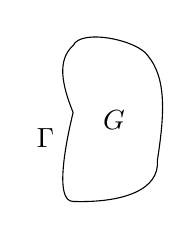
\begin{tikzpicture}[x=1cm,y=1cm]
\draw (0.30,0.10)
  .. controls (0.05,0.10) and (0.22,0.90) .. (0.30,1.23)
  .. controls (0.15,1.60) and (0.10,1.90) .. (0.30,2.08)
  .. controls (0.40,2.30) and (1.12,2.15) .. (1.25,1.95)
  .. controls (1.49,1.66) and (1.46,1.20) .. (1.37,0.62)
  .. controls (1.40,0.25) and (0.94,0.08) .. (0.30,0.10);
\node at (0.82,1.14) {$G$};
\node at (-0.05,0.91) {$\Gamma$};
\end{tikzpicture}
\end{adjustbox}
\end{center}

$A(x,\xi)$ — элл. символ.

Условие на изм. $A(x,\xi)$ вдоль границы.

\SourceFigure{GELFAND-P000203}{collar-diagram}{Слева: две близкие неровные овальные обводки, полоса между ними заполнена поперечными штрихами. Внутри — вытянутый тонкий контур с короткими штрихами, местами прерывистый. Подписей и явных стрелок внутри рисунка нет; замыкание тонкого внутреннего контура неясно.}

\begin{equation*}
\Gamma_\varepsilon=\Gamma\times[0,\varepsilon),
\quad \text{коорд. }(x',\xi',x_n,\xi_n)
\end{equation*}

\begin{gather*}
A(x,\xi)\\
a_+(x')=A(x',0,0,1)\\
a_-(x')=A(x',0,0,-1)\\
b(x')=a_+(x')^{-1}a_-(x')\quad\text{— мера неэлл.}\\
\gamma(x')=\frac{1}{2\pi i}\cdot\ln b(x')
\end{gather*}

\SourceFigure{GELFAND-P000203}{margin-arrows}{Слева от пунктов а), б) — две длинные почти параллельные вертикальные линии с наконечниками внизу. У верхнего конца левой линии и близ верхней части правой есть короткие боковые штрихи; неясно, являются ли они дополнительными наконечниками.}

а) Треб., чтобы ветви $\ln$ можно было выбрать
так, чтобы [зачёркнуто:
\Unclear{GELFAND-P000203}{cancelled-before-gamma}{на / их / неразборчиво}]
$\gamma_j(x')$ — были непр. на всем
\Unclear{GELFAND-P000203}{overwritten-boundary}{$\Gamma$ / переправленный неразборчивый знак}

(лок. это возм. всегда)

б) $|\operatorname{Re}\gamma_i(x')-\operatorname{Re}\gamma_j(x')|<1$ на $\Gamma$

Это класс
\Unclear{GELFAND-P000203}{elliptic-class}{$\widehat{\mathcal E}_\alpha$ или $\widehat{\varepsilon}_\alpha$}.

(При фикс. $x'$ можно — аргум. в один
интерв. \Unclear{GELFAND-P000203}{interval-symbol}{$1$ / $\lambda$ / стрелка вверх}
— надо, чтобы не расползались)

\begin{equation*}
\mathcal A=
\begin{pmatrix}
a_1(x,\xi)& &0\\
 &\ddots& \\
0& &a_p(x,\xi)
\end{pmatrix}
\end{equation*}

\SourcePage{GELFAND-P000204}{65}
% Original inspected at 2024 x 2415 pixels; enlarged review boxes are original-pixel (left,top,right,bottom), origin upper left.
% Review crops: top=(170,35,2005,570) at 3x; heading=(160,570,1945,1060) at 3x; hyperbolicity=(155,1020,1995,1455) at 3x; fundamental=(175,1420,1975,1835) at 3x; cones=(160,1815,1975,2385) at 3x.
% Further review: topword=(270,65,1305,176) at 4x; topline2=(285,165,1940,254) at 4x; line-this=(270,377,1390,457) at 4x; question=(745,462,1999,560) at 4x; top-formula=(615,252,1550,372) at 5x.
% Further review: cancel-hyper=(180,1020,284,1110) at 8x; coeff-real=(1583,916,1939,1023) at 5x; condition-word=(292,1585,493,1665) at 6x; cone-cancel=(355,1983,740,2100) at 6x.
% Further review: cone-note=(1532,2023,1948,2150) at 4x; last-phrase=(246,2280,1150,2383) at 4x; gamma-symbol=(1250,279,1529,373) at 7x; membership=(1454,455,1731,573) at 7x.

$a$: факторизуем —
\Unclear{GELFAND-P000204}{top-first-symbol}{$\kappa_j(x')$ / $\chi_j(x')$ / $x_j(x')$}.

$\gamma_j$ будут
\Unclear{GELFAND-P000204}{top-second-symbol}{$\kappa_j$ / $\chi_j$ / $x_j$}
и не получается этот класс.
\begin{equation*}
b=e^{2\pi i\kappa_j(x')},\qquad \gamma_j=\kappa_j
\end{equation*}
\Unclear{GELFAND-P000204}{top-exponential-symbol}{Знак, переданный $\kappa_j$: $\kappa_j$ / $\chi_j$ / $x_j$.}

Это для опер. в обычных пр-вах.

Осн. вопрос: когда глобально сущ.
\Unclear{GELFAND-P000204}{global-existence}{$G\in E$ / $G\notin E$ / $G\,\&\,E$ / $G$ и $E$; средний знак переписан}
(и $B$)?

\bigskip
27/III \quad \underline{Раб. Атийи в изл. С. Гельфанда.}

[Под заглавием:] (по Петровскому)

(Докл. №319 в сем. Бурбаки).

Рассм. однор. гиперб. ур-е с пост. коэффициентами
\begin{equation*}
Pu=\sum_{|\alpha|=m}a_\alpha D^\alpha u
\qquad \text{в }\mathbb{R}^{n}.
\end{equation*}
\Unclear{GELFAND-P000204}{ambient-dimension}{В источнике $\mathbb{R}^{n}$; далее индексы координат $0,\ldots,n$.}

[Справа, волнисто подчёркнуто:] $a_\alpha$ — веществ.

[Слева зачёркнуто:]
\Unclear{GELFAND-P000204}{cancelled-before-hyperbolicity}{$R^n$ или «На».}
Гиперболичность: (по $\xi_0$):
\begin{equation*}
\sum a_\alpha\xi^\alpha=a(\xi_0,\ldots,\xi_n)
\end{equation*}
$\forall$ ненулев. набора $(\xi_1,\ldots,\xi_n)\ne0$
\begin{equation*}
a(\xi_0,\ldots,\xi_n)=0
\end{equation*}
имеет ровно $m$ вещ. разл. корней.

Ищется реш. задачи
\begin{equation*}
\left\{
\begin{aligned}
Pu&=\delta(x_0,\ldots,x_n),\\
&\text{облад. доп. условием}\\
u&=0\quad\text{при }x_0<0.
\end{aligned}
\right.
\end{equation*}
[Справа:] Оно обозн. $E$ и только одно по теор. единств. реш. зад. Коши.

Известно, что оно устроено так:
\begin{equation*}
\text{Конус}\qquad a(\xi_0,\ldots,\xi_n)=0
\qquad A
\end{equation*}
К нему в пр-ве $(x_0,\ldots,x_n)$ — двойств. конус $B$.

[Ниже зачёркнуто:]
\Incomplete{GELFAND-P000204}{cancelled-cone-line}{неразборчиво; возможно «гиперпл.».}

[Справа, со штрихом к $B$:] конус гиперпл., кас. к $A$.
\begin{equation*}
b(x_0,\ldots,x_n)=0
\end{equation*}
Надо взять конус $B$, решение аналит. в $\forall$ связн. комп.
\Unclear{GELFAND-P000204}{last-word}{дополнения / дополнение}
$B$.

\SourcePage{GELFAND-P000205}{unlabelled}
% Original inspected at 2024 x 2415 pixels; no confidently readable page label visible.
% Enlarged review boxes are original-pixel (left,top,right,bottom), origin upper left.
% Review crops: top=(20,0,2005,400) at 3x; complex=(190,380,1990,1050) at 3x; cycles=(190,1030,1990,1490) at 3x; real=(190,1475,1990,1975) at 3x; wave=(220,1950,2010,2415) at 3x.
% Further review: cone-diagram=(1688,12,1848,199) at 8x; wave-last-index=(1513,2130,1656,2236) at 10x; wave-last-index-ax=(1713,2220,1898,2331) at 7x; equation-dash=(249,400,929,486) at 4x.
% Further review: manifold-word=(1117,586,1828,684) at 4x; parenthesis-complex=(241,770,1044,851) at 4x; cycle-property=(262,281,1937,375) at 3x.

Область [над строкой вписано: $C$] — лакуна, если $E(x)\equiv0$ на $C$.

[Под словом «Область»:] (св. комп.)

\SourceFigure{GELFAND-P000205}{upper-right-cone}{В правом верхнем углу конус вершиной вниз: сверху большой овальный контур, внутри малый замкнутый контур с двумя короткими вертикальными штрихами; несколько образующих сходятся в нижней вершине, правый внешний край утолщён. Внутренний знак и точное взаимное положение штрихов требуют проверки по источнику.}

\underline{Устойчивая лакуна} — если оно — лакуна для близких ур-й.

Есть необх. и дост. условие сущ. устойчив. лакуны —

— нек-рые циклы на алг. мн-зиях гомологичны нулю.

Ур-е $a=0$ —
\Unclear{GELFAND-P000205}{word-after-equation}{м / и}
\begin{equation*}
(\xi_0,\ldots,\xi_n)\subset\mathbb{C}P^n
\end{equation*}
\Unclear{GELFAND-P000205}{projective-relation}{Видимый знак перед $\mathbb{C}P^n$ похож на $\subset$; возможно $\in$.}
\begin{equation*}
a(\xi)=0\quad\text{— выделяет мн-зие }A\text{ (компл.)}
\end{equation*}
Предполагается, что уже в $\mathbb{C}P^n$ оно неособое
(нет компл. особых точек).

Этого всегда можно добиться вещ. изменением коэфф.
(небольшим).
\begin{equation*}
A_{\mathbb{R}}=A\cap\mathbb{R}P(n)
\end{equation*}
Пусть есть точка
$\begin{gathered}x\\ \Vert\\ (x_0,\ldots,x_n)\end{gathered}$.
Построим по ней 2 цикла

1.
\begin{equation*}
x_0\xi_0+x_1\xi_1+\ldots+x_n\xi_n=0
\quad\text{— плоскость (компл.)}
\end{equation*}
\begin{equation*}
A_x=A\cap\{(x,\xi)=0\}
\end{equation*}
[Под $A_x$ вертикальный штрих к словам:] тоже есть вещ. часть
\begin{equation*}
(A_x)_{\mathbb{R}}=A_x\cap\mathbb{R}P(n);
\qquad \text{его }\dim=n-2
\end{equation*}
Это цепь в гомологиях (цикл) — сумма сфер:
\begin{equation*}
\underline{\beta_x\in H_{n-2}(A_x)}
\end{equation*}

\underline{Для волнов. ур-я.}
\begin{equation*}
\frac{\partial^2}{\partial x_0^2}-\Delta u
\end{equation*}
\Unclear{GELFAND-P000205}{wave-operator-source}{В числителе написано $\partial^2$ без $u$; после минуса написано $\Delta u$.}
\begin{equation*}
x=(1,0,\ldots,0).
\qquad
A=\{\xi_0^2-\xi_1^2-\ldots-\xi_n^2=0.\}
\end{equation*}
\begin{equation*}
A_x:\quad \xi_0=0\Rightarrow
A_x=\{\xi_1^2+\ldots+\xi_n^2=0\}\quad\text{—}
\end{equation*}
— в проект. пр-ве это будет 0 (нет точек)
\Unclear{GELFAND-P000205}{empty-projective-locus}{В последней строке не указано, идёт ли речь о вещественной части $A_x$.}

\SourcePage{GELFAND-P000206}{66}
% Direct review: original PNG 2024 x 2415 inspected at source resolution.
% Review crop coordinates are original pixels (left, top, right, bottom), origin upper-left; right/bottom exclusive.
% Review crops: top-main=(80,95,1245,425), 3x; top-note=(1250,112,1905,565), 3x.
% Review crops: middle-upper=(90,422,1830,899), 3x; middle-cancel=(154,883,1875,1300), 3x.
% Review crops: theorem=(82,1300,1860,1735), 3x; bottom-form=(120,1700,1870,2135), 3x; bottom=(110,2080,1795,2415), 3x.
% Review crops: small-cancel=(1300,785,1385,869), 10x; cancel-index=(952,971,1222,1068), 10x.
% Review crops: relative-ax=(1188,644,1525,747), 6x; chain-dim=(433,423,597,507), 8x.
% Review crops: bad-section=(943,2318,1310,2413), 5x; cycles-membership=(546,316,965,398), 6x.
% Review crop: top-alpha-cancel=(900,216,1228,279), 8x.
% Independent comparison: Разобьем (without dots over е), source box (1290,208,1487,274), reviewed within top-note crop at 3x.

2. Другой цикл.

Рассм. отобр.
\begin{gather*}
\xi\mapsto\operatorname{sign}(x,\xi),\\
\xi\in A_R,
\end{gather*}
[Зачёркнуто двумя горизонтальными линиями: $\alpha$ — цикл.]

[Зачёркнуто накрест: $\partial\alpha\in(A_R)_x$.]

[Справа от вертикальной черты:]
\begin{quote}
Оно даёт цикл.
Разобьем $A_R$ плоск.
$(x,\xi)$ на 2 части
и одну с $+$, другую
с $-$.
\begin{gather*}
\{(x,\xi)>0\}-\{(x,\xi)<0\}\\
(a\in C_{n-1}(A))
\end{gather*}
\end{quote}

Получ. $(n-1)$-мерн. цепь на $A$
$(C_{n-1}(A))$
\begin{equation*}
\partial a\in(A_x)_R\quad\text{— цикл}
\end{equation*}

Поэтому опр. элем.
\Unclear{GELFAND-P000206}{relative-ax}{$\alpha_x\in H_{n-1}(A,Ax)$; второй аргумент: $Ax$ или $A_x$}
и из точн. посл. гомологий:

$\partial\alpha_x\in H_{n-2}(A_x)$
[Зачёркнуто: \Unclear{GELFAND-P000206}{boundary-cancel}{«и», $H$ или иной знак}],
$\partial\alpha_x=2\beta_x$.

Если $x$ мен. в связн. комп. доп. конуса, то
$\alpha_x$, $\beta_x$ не меняются.
\Unclear{GELFAND-P000206}{cancelled-homology-index}{[Зачёркнуто: «(в $H_{n-\ldots}$)»; индекс неразборчив.]}

$\alpha_c$, $\beta_c$ — соотв. циклы. (элем. гомологий).
\begin{equation*}
\alpha_c\in H_{n-1}(A,A_c),\qquad
\beta_c\in H_{n-2}(A_c)
\end{equation*}

\underline{Теорема}. $m$ — пор. ур-я, $n+1$ — разм. пр-ва,
$m$, $n+1$ чётны.

а) $m\ge n+1\Rightarrow\alpha_c=0$ — необх. и дост. условие,
чтобы $c$ было уст. лакуной

б) $m<n+1\Rightarrow\beta_c=0$ — [Два ряда знаков повтора слов
«необх. и дост. условие, чтобы $c$ было уст. лакуной».]

\underline{Док-во}: явный вид $E$.

На $CP(n)$ рассм. форму типа $(n,0)$ (голоморфную)
с единств. полюсом пор. $(n+1)$ (она единств.)
\begin{equation*}
\Omega\cong O(-n-1)
\end{equation*}
[Под $\Omega$ короткая черта к подписи: голом. формы.]

Глоб. рег. сечений нет. (отсюда единств.)
\begin{equation*}
\omega=x_0\,dx_1\wedge\ldots\wedge dx_n
-x_1\,dx_0\wedge dx_2\wedge\ldots
\end{equation*}
— (в афф. пр-ве) — площ. сферы.

\SourcePage{GELFAND-P000207}{unlabelled}
% Direct review: original PNG 2024 x 2415 inspected at source resolution. Writing occupies the upper part; remainder is blank.
% Review crop coordinates are original pixels (left, top, right, bottom), origin upper-left; right/bottom exclusive.
% Review crops: top-left=(227,12,1404,221), 3x; top-condition=(1410,84,1918,218), 3x.
% Review crops: formula=(331,248,1590,522), 3x; note=(310,523,955,642), 3x.
% Review crops: condition-a=(1760,99,1900,187), 10x; name=(941,244,1586,322), 5x; theta=(1047,98,1104,186), 10x.

Использ. форма-вычет $\omega_a$ на пов. $a=0$.
\begin{equation*}
\frac{\omega}{a}=\frac{da}{a}\wedge\omega_a+\Theta
\end{equation*}
\Unclear{GELFAND-P000207}{residue-remainder}{Обозначение последнего слагаемого и в следующей скобке: $\Theta$ или $\theta$.}

($\Theta=0$ на
\Unclear{GELFAND-P000207}{residue-condition}{$a=0$ или $a=\varphi$})
[Скобка и её содержимое подчёркнуты волнистой линией.]

$m\ge n+1$ — ф-ла Герглотца—Петровского
\begin{equation*}
E(x)=c\int_{A_R}\operatorname{sgn}(x,\xi)(x,\xi)^{m-n-1}\omega_a
\end{equation*}

(см. 1-й выпуск)
[Под строкой: об. ф-й.]

\end{document}
